\documentclass[12pt]{osuthesis}
\usepackage[letterpaper, margin=1in]{geometry}

%%%%%%%%%%%%%%%%%%%%%%%%%%%%%%%%%%% NOTICE %%%%%%%%%%%%%%%%%%%%%%%%%%%%%%%%%%%
% BASIC INSTRUCTIONS:
% Find the sections marked with a NOTICE of this form and fill in the relevant
% information. You will then put the substance of your thesis in the separate
% chapter TeX files. Remember, you will always compile THIS file.

% Warnings on using this file:
% - osuthesis.cls is not currently compatible with the hyperref package.
% - Do not include package amsthm, \qed and such commands are already
%   defined in osuthesis

%%%%%%%%%%%%%%%%%%%%%%%%%%%%%%%%%%%%%%%%%%%%%%%%%%%%%%%%%%%%%%%%%%%%%%%%%%%%%%


\usepackage{amsmath,amssymb}
\usepackage{comment}
\usepackage{enumerate}
\usepackage{mathrsfs}
\usepackage{fancyhdr}
\usepackage{changepage}
\usepackage{afterpage}
\usepackage[titles]{tocloft}

\usepackage{chngcntr}

\usepackage{mathtools}
\usepackage{graphicx}
\usepackage{soul}
\usepackage[short]{optidef}
\usepackage{multirow}
\usepackage[hidelinks]{hyperref}
\usepackage[natbibapa,nodoi]{apacite}
% \usepackage[numbers,sort]{natbib}
% \usepackage{apacite}
% \usepackage{amsmath,amsthm,amsfonts,mathtools,amssymb}
\usepackage[linesnumbered,ruled,vlined]{algorithm2e}
\usepackage{enumerate}
\usepackage{textcomp}
\usepackage{mathabx}
\usepackage{tabularx}
\usepackage{numprint}
\npthousandsep{,}
\usepackage{booktabs} 
\usepackage{float}
\usepackage{enumerate}
\usepackage{xcolor}
\usepackage{float}
\usepackage{booktabs}
\usepackage{multirow,multicol,threeparttable}
\usepackage{longtable}

\usepackage{lscape}
\usepackage{afterpage}

\newcommand{\alert}{\textcolor{red}}
\newcommand{\comm}{\textcolor{blue}}
\newcommand{\review}{\textcolor{magenta}}




%%%%%%%%%%%%%%%%%%%%%%%%%%%%%%%%%%% NOTICE %%%%%%%%%%%%%%%%%%%%%%%%%%%%%%%%%%%
% If you want your tables and/or figures to be numbered within chapter and section,
% change the following two commands to \counterwithin instead of \counterwithout:
\counterwithout{figure}{chapter}
\counterwithout{table}{chapter}

\renewcommand{\cftchapaftersnum}{.}


%%%%%%%%%%%%%%%%%%%%%%%%%%%%%%%%%%% NOTICE %%%%%%%%%%%%%%%%%%%%%%%%%%%%%%%%%%%
% Make any of these widths wider if needed
\renewcommand*\cftchapnumwidth{3.5em}
\renewcommand*\cftsecnumwidth{3.4em}
\renewcommand*\cftsubsecnumwidth{4em}
% The second argument (1.5em) is the space before the
% I.1 entry for the figure/table
% The third argument (4em) is the space to allow for the I.1
% style entry.

\newtheorem{claim}{Claim}
\newtheorem{theo}{Theorem}
\DeclareMathOperator{\SCI}{SCI}
\newcommand{\suchthat}{\;\ifnum\currentgrouptype=16 \middle\fi|\;}
\newcommand{\conv}{\operatorname{conv}}
\newcommand{\proj}{\operatorname{proj}}
\newcommand{\pv}{\mathscr{P}_V}
\newcommand{\np}{$\mathcal{NP}$}
\def\hsymb#1{\mbox{\strut\rlap{\smash{\Huge$#1$}}\quad}}
% THINGS FOR TIKZ
\usepackage{tikz,tkz-graph}
\usetikzlibrary{arrows,automata,shapes.geometric,arrows}
\tikzstyle{vertex}=[circle, draw, inner sep=0pt, minimum size=6pt]
\newcommand{\vertex}{\node[vertex]}
\usetikzlibrary{shapes.misc, positioning}
\allowdisplaybreaks[1]

\tikzstyle{startstop} = [rectangle, rounded corners, minimum width=3cm, minimum height=1cm,text centered, draw=black, fill=red!30]

\tikzstyle{arrow} = [thick,-,>=stealth]

\newtheorem{Theorem}{Theorem}[section]
\newtheorem{lem}{Lemma}[Theorem]
\newtheorem{prop}{Proposition}[section]
%%%%%%%%%%%%%%%%%%%%%%%%%%%%%%%%%%%%%%%%%%%%%%%%%%%%%%%%%%%%%%%%%%%%%%%%%%%%%%


\makeatletter
%\renewcommand*\l@figure{\@dottedtocline{1}{1.5em}{4em}}
%\renewcommand*\l@table{\@dottedtocline{1}{1.5em}{4em}}
\makeatother
%%%%%%%%%%%%%%%%%%%%%%%%%%%%%%%%%%%%%%%%%

%  change the format of labels in equations and chapters 
\renewcommand{\thechapter}{\Roman{chapter}}
\renewcommand{\theequation}{\thechapter.\arabic{equation}}
\counterwithin*{equation}{chapter}


%%%%%%%%%%%%%%%%%%%%%%%%%%%%%%%%%%% NOTICE %%%%%%%%%%%%%%%%%%%%%%%%%%%%%%%%%%%
% Put your shortcuts for math symbols etc. that you want to use here in this
% section. They will be available in every chapter file afterwards.
% Some example shortcuts are included below.
\def\A{{\mathbb A}}
\def\C{{\mathbb C}}
\def\D{{\mathbb D}}
\def\K{{\mathbb K}}
\def\L{{\mathbb L}}
\def\N{{\mathbb N}}
\def\Q{{\mathbb Q}}
\def\R{{\mathbb R}}
\def\Z{{\mathbb Z}}
\def\E{{\mathbb E}}
\def\T{{\mathbb T}}
\def\P{{\mathbb P}}
\def\S{{\mathbb S}}
\def\nn{\mathbf{n}}
\newcommand{\cE}{\mathcal{E}}
\newcommand{\cF}{\mathcal{F}}
\def\eps{\varepsilon}
\def\vp{\varphi}
\newcommand{\ds}{\displaystyle{}}
\newcommand{\abs}[1]{\left\lvert#1\right\rvert}
\newcommand{\BigO}[1]{\ensuremath{\operatorname{O}\bigl(#1\bigr)}}
\newcommand{\defeq}{\mathrel{\mathop:}=}
\newcommand{\Var}{\mathrm{Var}}
\newcommand{\Cov}{\mathrm{Cov}}
\DeclareMathOperator{\csch}{csch}
\newcommand{\overbar}[1]{\mkern 1.5mu\overline{\mkern-1.5mu#1\mkern-1.5mu}\mkern 1.5mu}
\newcommand{\Sp}{\mathbb S}
\newcommand{\cp}{\operatorname{cap}}
\newcommand{\dist}{\operatorname{dist}}
\newcommand{\interi}{\operatorname{int}}
\newcommand{\norm}[1]{\left\lVert#1\right\rVert} % norm: double vertical bars
\newcommand{\Beta}{{\rm B}}
\newcommand{\sn}{{\rm sn}}
\newcommand{\cn}{{\rm cn}}
\newcommand{\dn}{{\rm dn}}
\newcommand{\Ec}{{\rm Ec}}
\newcommand{\Es}{{\rm Es}}
%%%%%%%%%%%%%%%%%%%%%%%%%%%%%%%%%%%%%%%%%%%%%%%%%%%%%%%%%%%%%%%%%%%%%%%%%%%%%%

%commands: \added{}, \deleted{}, and \replaced{}{} will automatically keep track of the changes and also show the changes in blue.
% \usepackage{tablefootnote}
% \usepackage{amsmath}
% \usepackage{amssymb}
% \usepackage{calrsfs}


% \usetikzlibrary{shapes, arrows}
% \usetikzlibrary{positioning}

% \newcommand{\vertex}{\node[vertex]}
% \newcommand{\rl}{\mathbb{R}}
\newcommand{\calF}{\mathcal{F}}
% \newcommand{\calS}{\mathcal{S}}
\newcommand{\calH}{\mathcal{H}}
% \newcommand{\calD}{\mathcal{D}}
\newcommand{\calX}{\mathcal{X}}
% \newcommand{\calE}{\mathcal{E}}
% \newcommand{\calR}{\mathcal{R}}
% \newcommand{\indic}{\mathbbm{1}}
\newcommand{\true}{\texttt{true}}
\newcommand{\false}{\texttt{false}}
\newcommand{\flag}{\texttt{flag}}
\newcommand{\Or}{\texttt{or}}

\SetKw{Continue}{continue}
\SetKw{Break}{break}
\DeclareMathOperator*{\den}{den}
\DeclareMathOperator*{\num}{num}
% \DeclareMathOperator*{\diam}{diam}
% \DeclareMathOperator*{\dist}{dist}
% \DeclareMathOperator*{\val}{value}
% \DeclareMathOperator*{\visited}{visited} 
% \DeclareMathOperator*{\vnbr}{is-v-nbr} 
% \DeclareMathOperator{\bigO}{\mathcal{O}}

% % define problem statement
% \newcommand\prob[3]{%
%  \vspace{2mm}
%   \par\noindent {\bf Problem}: #1.\\
%   {\bfseries Input}: #2.\\
%   {\bfseries Output}: #3.\par
%  \vspace{2mm}
% }

\newcommand\probd[3]{%
 \vspace{2mm}
  \par\noindent {\bf Problem}: \textsc{#1}\\
  {\bfseries Instance}: #2.\\
  {\bfseries Question}: #3?\par
 \vspace{2mm}
}


% Natbib setup for author-year style
\usepackage{natbib}
 \bibpunct[, ]{(}{)}{,}{a}{}{,}%
 \def\bibfont{\small}%
 \def\bibsep{\smallskipamount}%
 \def\bibhang{24pt}%
 \def\newblock{\ }%
 \def\BIBand{and}%




%%%%%%%%%%%%%%%%%%%%%%%%%%%%%%%%%%%%%%%%%%%%%%%%%%%%%%%%%%


\makeatletter
\newcommand\Dotfill{\leavevmode \cleaders \hb@xt@ 1.1em{\hss .\hss }\hfill \kern \z@}
\makeatother


\suppressfloats %\nofiles

\newcommand{\supp}{\mathop{{\rm supp}}}
\newcommand{\esssup}{\mathop{{\rm ess\,sup}}}

\renewcommand{\appendixname}{Appendix}


%%%%%%%%%%%%%%%%%%%%%%%%%%%%%%%%%%% NOTICE %%%%%%%%%%%%%%%%%%%%%%%%%%%%%%%%%%%
% Fill in your title and other information here.

\title{Fractional Programming Framework for Cluster Discovery in Healthcare Analytics}
\formattedtitle{FRACTIONAL PROGRAMMING FRAMEWORK FOR CLUSTER DISCOVERY IN HEALTHCARE ANALYTICS}

\author{PARISA VAGHFI MOHEBBI}

\degreeone{\ssp Bachelor of Science in Mathematics and Applications\\
Amirkabir University of Technology (Tehran Polytechnic)\\
Tehran, Iran\\
        2017}

\degreetwo{\ssp Master of Science in Applied Mathematics - Optimization\\
Amirkabir University of Technology (Tehran Polytechnic)\\
Tehran, Iran\\
2019}


\degreesought{DOCTOR OF PHILOSOPHY}
 \degreedate{June, 2026}
\majorfield{Industrial Engineering and Management}

%%%%%%%%%%%%%%%%%%%%%%%%%%%%%%%%%%%%%%%%%%%%%%%%%%%%%%%%%%%%%%%%%%%%%%%%%%%%%%


\begin{document}

\maketitle

\makecopyright

%%%%%%%%%%%%%%%%%%%%%%%%%%%%%%%%%%% NOTICE %%%%%%%%%%%%%%%%%%%%%%%%%%%%%%%%%%%
% Put your advisor's and the committee members' names here:
\makeapproval{Dr.~Balabhaskar Balasundaram}{Dr.~Austin Buchanan}{Dr.~Akash Deep}{Dr.~Ramesh Sharda}


\begin{dedication}
Dedicated to my mother
\end{dedication}

\begin{acknowledge}
 I would like to thank my advisor, Dr.~Balasundaram, for his guidance
throughout this dissertation, and my committee members,
Dr.~Buchanan, Dr.~Deep, and Dr.~Sharda, for their time and feedback.

I am grateful to my mother and brother for their unwavering love,
encouragement, and support throughout my doctoral studies. Their
belief in me has been a source of strength and motivation.

I also wish to acknowledge the opportunity to pursue and complete my doctoral education in the United States of America.

The computing for this dissertation was performed at the High Performance Computing Center at Oklahoma State University (HPC Pete), supported in part through the National Science Foundation grant OAC-1126330.

%%%%%%%%%%%%%%%%%%%%%%%%%%%%%%%%%%% NOTICE %%%%%%%%%%%%%%%%%%%%%%%%%%%%%%%%%%%
% If you Acknowledgments span MORE than one page, the graduate college
% requires that you have this footer present on every page. In order to put it
% there, you will put this footer command in some of the text on page 2 (or 3,
% etc.) in order to ensure a copy of the footer appears on each page:

%\blfootnote{Acknowledgments reflect the views of the author and are not endorsed
% by committee members or Oklahoma State University.}

%%%%%%%%%%%%%%%%%%%%%%%%%%%%%%%%%%%%%%%%%%%%%%%%%%%%%%%%%%%%%%%%%%%%%%%%%%%%%%

\end{acknowledge}

%%%%%%%%%%%%%%%%%%%%%%%%%%%%%%%%%%% NOTICE %%%%%%%%%%%%%%%%%%%%%%%%%%%%%%%%%%%
% Fields passed to abstract are:
% Name, Month and Year of Graduation, Title, Field, and spacing: Use 0in or 1in per GC policy,
% depending on length of the abstract. A longer abstract will 0in, a shorter abstract 1in.

\begin{abstract}{PARISA VAGHFI MOHEBBI}
{June, 2026}
{FRACTIONAL PROGRAMMING FRAMEWORK FOR CLUSTER DISCOVERY IN HEALTHCARE ANALYTICS}
{INDUSTRIAL ENGINEERING AND MANAGEMENT}
{1in}
   %Abstract will go here.  Make sure it remains within the 350 word limit.
%\par To get a new paragraph
\par This dissertation studies the problem of identifying disease clusters
associated with the highest mortality rates among patients in
electronic health record databases. We introduce the maximum
mortality rate clique problem, a fractional combinatorial
optimization problem defined on a comorbidity graph whose vertices are
disease categories and whose edges reflect statistically significant
pairwise co-occurrence. The problem seeks a frequent clique, supported
by a sufficiently large shared patient population, that maximizes the
mortality rate of the patients simultaneously diagnosed with all
diseases in the clique.
\par We establish that the mortality rate function is neither additive nor
monotonic, ruling out simple greedy strategies, and prove
NP-completeness of the core decision problem and several related
variants. These results motivate the development of exact solution
methods of increasing sophistication.
\par We develop two exact combinatorial algorithms: a modified
Bron--Kerbosch enumerative algorithm and a combinatorial
branch-and-bound algorithm that incorporates an upper-bounding scheme
to prune the search tree aggressively. We present two mixed-integer
linear programming formulations based on auxiliary product-variable
linearization and the Charnes--Cooper transformation. These
formulations become intractable as the patient population grows. To
overcome this, we introduce a logic-based Benders decomposition
reformulation that eliminates all patient-indexed variables and embeds
naturally in a decomposition branch-and-cut framework. A hybrid
variant further integrates the combinatorial branch-and-bound
algorithm to generate stronger valid inequalities, substantially
improving solution times and optimality gaps over the pure
logic-based Benders decomposition approach.
\par We further extend the framework to incorporate side constraints, a
size-restricted variant, and a marginal mortality rate variant. We
evaluate all proposed methods using the real-world electronic health
record dataset MIMIC-IV.
\end{abstract}
%%%%%%%%%%%%%%%%%%%%%%%%%%%%%%%%%%%%%%%%%%%%%%%%%%%%%%%%%%%%%%%%%%%%%%%%%%%%%%


\renewcommand{\listfigurename}{LIST OF FIGURES}
\renewcommand{\listtablename}{LIST OF TABLES}

{\addtocontents{toc}{\protect\renewcommand{\protect\cftchapleader}
 {\protect\cftdotfill{\cftsecdotsep}}} %<-adds leaders at the chapter level
\addtocontents{toc}{~{\kern-0.3in Chapter}\hfill{Page}\par} %<-this line deals with the first toc page

\fancypagestyle{fancyplain}{ %
 \lhead{ \fancyplain{}{Chapter} }
 \rhead{ \fancyplain{}{Page} }
 \renewcommand{\headrulewidth}{0pt} % remove lines which fancyhdr usually uses
 \renewcommand{\footrulewidth}{0pt}
}

\changepage{-29.43001pt}{}{}{}{}{}{15pt}{12pt}{}
\pagestyle{fancyplain}
\thispagestyle{plain}
\tableofcontents
}

\renewcommand{\cftfigaftersnum}{.}
\renewcommand{\cfttabaftersnum}{.}

%%% Generate the list of tables
\fancypagestyle{fancyplain}{ %
 \lhead{ \fancyplain{}{Table} }
 \rhead{ \fancyplain{}{Page} }
 \renewcommand{\headrulewidth}{0pt} % remove lines as well
 \renewcommand{\footrulewidth}{0pt}
}
\changepage{-29.43001pt}{}{}{}{}{}{15pt}{12pt}{}
\pagestyle{fancyplain}\renewcommand{\thepage}{\roman{page}}
\thispagestyle{plain}\renewcommand{\thepage}{\roman{page}}
\ssp
%%%%%%%%%%%%%%%%%%%%%%%%%%%%%%%%%%% NOTICE %%%%%%%%%%%%%%%%%%%%%%%%%%%%%%%%%%%
% Comment this line out if you do not want a List of Tables:
\listoftables
%%%%%%%%%%%%%%%%%%%%%%%%%%%%%%%%%%%%%%%%%%%%%%%%%%%%%%%%%%%%%%%%%%%%%%%%%%%%%%


%%% Generate the list of figures
\fancypagestyle{fancyplain}{ %
 \lhead{ \fancyplain{}{Figure} }
 \rhead{ \fancyplain{}{Page} }
 \renewcommand{\headrulewidth}{0pt} % remove lines as well
 \renewcommand{\footrulewidth}{0pt}
}
\pagestyle{fancyplain}\renewcommand{\thepage}{\roman{page}}
\thispagestyle{plain}\renewcommand{\thepage}{\roman{page}}
\ssp

%%%%%%%%%%%%%%%%%%%%%%%%%%%%%%%%%%% NOTICE %%%%%%%%%%%%%%%%%%%%%%%%%%%%%%%%%%%
% Comment this line out if you do not want a List of Figures:
\listoffigures
%%%%%%%%%%%%%%%%%%%%%%%%%%%%%%%%%%%%%%%%%%%%%%%%%%%%%%%%%%%%%%%%%%%%%%%%%%%%%%

\pagestyle{plain}

\changepage{27pt}{}{}{}{}{}{-15pt}{-12pt}{} % Reset headers height to zero and restore textheight
\dsp

%%%%%%%%%%%%%%%%%%%%%%%%%%%%%%%%%%% NOTICE %%%%%%%%%%%%%%%%%%%%%%%%%%%%%%%%%%%
% Optional: uncomment the following lines if you want to include a Nomenclature page,
% and create TeX file notation.tex to use.
% \begin{nomenclature}
%  \input{nomenclature}
% \end{nomenclature}

%%%%%%%%%%%%%%%%%%%%%%%%%%%%%%%%%%% NOTICE %%%%%%%%%%%%%%%%%%%%%%%%%%%%%%%%%%%
% Optional: uncomment the following 3 lines if you want to include a list of symbols page
% \begin{listofsymbols}
%  \input{listofsymbols}
% \end{listofsymbols}

\newpage
\pagenumbering{arabic}\setcounter{page}{1}

%%%%%%%%%%%%%%%%%%%%%%%%%%%%%%%%%%% NOTICE %%%%%%%%%%%%%%%%%%%%%%%%%%%%%%%%%%%
% This is where you will put your thesis chapters files. You do not need to
% include the .tex extension, but this input command is inputing chapter1.tex,
% etc.
\begingroup
\clearpage
\let\clearpage\relax
\vspace*{-40pt}
\chapter[BACKGROUND AND MOTIVATION]{BACKGROUND AND MOTIVATION}\label{sec.background}
\endgroup

This chapter motivates the study undertaken in this dissertation and covers necessary background.
Section~\ref{sec.ehr} introduces the role of electronic health records
in comorbidity analysis and mortality risk assessment.
Section~\ref{sec.mcp} reviews classical and modern approaches to the
maximum clique problem. Section~\ref{sec.fp} surveys fractional
programming and its integer and combinatorial extensions.
Section~\ref{sec.contributions} summarizes the contributions of this
dissertation.

\section{Electronic Health Records in Comorbidity and Mortality
Analysis}\label{sec.ehr}

Electronic health records (EHRs) capture comprehensive longitudinal
patient information, including demographics, diagnoses, medications,
laboratory results, and procedures. These rich, multimodal datasets
support large-scale cohort studies, knowledge discovery, and the
development of longitudinal phenotypic profiles that inform clinical
decision-making and personalized medicine~\citep{Jensen2012}. They
have become indispensable for healthcare analytics, enabling advanced
data mining techniques such as information extraction, representation
learning, outcome prediction, phenotyping, de-identification, disease
prediction, comorbidity analysis, and patient
stratification~\citep{Yadav2018,Sarwar2023}.

The widespread adoption of EHR systems, accelerated by initiatives
such as the U.S. Health Information Technology for Economic and
Clinical Health Act of 2009, has produced vast repositories of
structured and unstructured data. By 2015, 84\% of hospitals and 87\%
of office-based physicians had implemented certified EHR
systems~\citep{Shickel2018}. This expansion has extended EHR utility
beyond primary functions such as billing and documentation to
secondary applications in clinical informatics, including the
extraction of medical concepts from clinical notes~\citep{Sarwar2023},
learning robust patient representations for predictive
modeling~\citep{Shickel2018}, forecasting outcomes such as hospital
readmission or heart failure~\citep{Yadav2018}, and automating
phenotyping for research cohort selection~\citep{Jensen2012}.

\textit{Mortality rate}, the fraction of deceased patients among those
with a particular disease or group of diseases, is a metric of broad
interest in medicine, epidemiology, and public health. The co-occurrence of multiple diseases in a single patient is often described using the related concepts of \textit{comorbidity} and \textit{multimorbidity}. Comorbidity refers to the presence of one or more additional conditions alongside a primary or index disease, whereas multimorbidity refers to the coexistence of two or more chronic conditions in an individual without designating any condition as primary. Comorbidity assumes particular significance in the context of mortality, as the interaction between two or more diseases can produce health outcomes that differ from those of each
disease in isolation~\citep{FEINSTEIN1970455}. Among the many
analytical opportunities offered by EHRs, comorbidity analysis stands
out as especially valuable for understanding mortality risk since
co-occurring diseases often interact in ways that elevate mortality
well beyond the simple additive effects of individual
conditions~\citep{FEINSTEIN1970455}. As \cite{Redelmeier1998}
highlight, a dominant illness can overshadow concurrent conditions and
increase the risk of clinical neglect, a challenge that data-driven
EHR analytics can help address.

Identifying multimorbidities in the form of disease clusters with high
mortality rates yields benefits across epidemiology, health policy,
healthcare management, and public health planning. Knowledge of such
clusters enables healthcare providers to anticipate disease onset early
and intervene proactively, improving the likelihood of successful
treatment and reducing mortality. It also supports more efficient
resource allocation, as health system administrators can direct
resources toward conditions most likely to lead to death. Furthermore,
high-mortality cluster identification can catalyze research into
underlying causes and potential treatments, and public health officials
can use this information to design targeted interventions for
high-risk populations.

\cite{Gijsen2001} conducted a comprehensive review of the causes and
consequences of comorbidity, finding that comorbidity was consistently
associated with increased mortality. Prior research indicates that
patients diagnosed with conditions such as myocardial infarction,
diabetes, chronic obstructive pulmonary disease, chronic kidney
disease, dementia, depression, hip fracture, stroke, colorectal
cancer, and lung cancer are at elevated risk of developing heart
failure~\citep{Ahluwalia2012}, a particularly notable link given that
heart disease and cancer account for the majority of reported deaths
in the United States~\citep{Xu2016}. \cite{Braunstein2003} further
show that elderly patients with chronic heart failure often succumb to
non-cardiac conditions, suggesting that identifying and addressing
these conditions can improve outcomes. \cite{CORRAINI2018242}
investigated the impact of comorbidity on post-stroke mortality in a
population-based cohort study, finding that conditions such as cancer,
advanced renal disease, or liver disease significantly increased
one-year mortality following a stroke.

Analytical approaches to mortality and comorbidity have historically
relied on statistical methods, with EHR data now enabling more
granular, longitudinal investigations. Early work by \cite{lu1996}
introduced a mixed Poisson regression model for age-specific and
age-standardized mortality rates, using a marginal quasi-likelihood
approach within an empirical Bayes framework to improve practical
analysis, particularly for diseases such as lung cancer.
\cite{LU2021113583} modeled comorbidities as temporal disease networks
to visualize comorbidity progression and identify critical transition
points using clustering techniques. More recent studies have
incorporated comorbidities to enhance predictive performance. For
example, \cite{ZOLBANIN2015150} demonstrated that including
comorbidities improves survival prediction models for cancer patients,
while gender-focused analyses have explored related
factors~\citep{Short2013S93}. Many investigations target comorbidities
linked to specific conditions, including diabetes, obesity, and
cancer~\citep{Holguin2005, Marrie2015, Leontiadis2013}.
\cite{vanGestel2013} found that comorbidity burden and advanced age
were associated with early postoperative mortality in gastrointestinal
cancer patients, with cardiovascular diseases exerting a particularly
strong effect on 30-day mortality. \cite{Koskinen2022} employed a
data-driven approach to analyze comorbidity patterns across a range of
common diseases, identifying disease-specific patient subgroups with
distinctive diagnosis patterns, survival functions, and laboratory
correlates, underscoring the heterogeneity within disease populations
and the need for personalized risk assessment.

Recent EHR-based studies have employed association rule mining (e.g. the a priori algorithm) and $k$-means clustering to uncover
frequent disease co-occurrences and support early detection and
tailored treatment~\citep{HariEtAl2024INFORMStutorial,Parisa2025}.
Optimization frameworks offer additional promise by formulating complex
analytical tasks as constrained problems. \cite{Zhong2022} modeled
relational-sequential patient clustering with custom distance measures
that account for demographic hierarchies and temporal diagnosis
similarity, producing clinically interpretable clusters. Similarly,
\cite{VaghfiMohebbi2025lethalclique} defined the maximum mortality
rate clique problem and applied enumeration to identify high-mortality
disease cliques in comorbidity graphs. 

The following section reviews the maximum clique problem and related solution methods that underpin this line of work.

\section{The Maximum Clique Problem}\label{sec.mcp}

A \emph{clique} in an undirected graph $G=(V,E)$ is a subset of
vertices in which every pair is connected by an edge. The \emph{maximum
clique problem} (MCP) asks for the largest such subset, i.e., the
clique of maximum cardinality. Closely related are the \emph{maximum
independent set problem} (MIS), which seeks the largest subset of
mutually non-adjacent vertices (also known as the stability number),
and the \emph{minimum vertex cover problem}, which seeks the smallest
set of vertices incident to every edge. These three problems are
equivalent in the following sense: a set $S$ is a maximum clique in
$G$ if and only if $S$ is a maximum independent set in the complement
graph $\bar{G}$, and if and only if $V \setminus S$ is a minimum
vertex cover in $\bar{G}$. This equivalence has enabled substantial
transfer of algorithmic ideas and bounding techniques across
all three problems~\citep{Bomze99survey}.

All three problems are NP-hard on general graphs~\citep{GareyJohnson79},
which has motivated a rich body of research on both exact and
approximate solution methods. The maximum clique problem admits several
natural integer programming formulations. The most basic is the
edge formulation, which maximizes the number of selected
vertices subject to pairwise incompatibility constraints derived from
the complement graph:
\begin{subequations}\label{form.eclique}
    \begin{align}
        \max &\ \sum_{i=1}^n x_i \label{ec.obj}\\
        \text{s.t.}\quad
        & x_i + x_j \le 1 && \forall \{i,j\} \in E(\bar{G})
            \label{ec.constraint}\\
        & x_i \in \{0,1\} && \forall i \in V(G).
    \end{align}
\end{subequations}
In formulation~\eqref{form.eclique}, $x_i=1$ means vertex $i$ is in the clique, and the constraint forbids selecting both endpoints of any non-edge, so any feasible binary solution corresponds to a clique. 
% \comm{You defined a clique a subset of nodes; so a binary vector cannot be one.}

More advanced mixed-integer formulations---including
clique-inequality-based, independent-set-augmented, and lifted
variants---have been developed to strengthen the LP relaxation and
improve branch-and-bound performance; a detailed comparison of their
strength and computational behavior appears in~\citep{Naderi2022}.
Earlier works explored quadratic programming representations and
exploited the Motzkin--Straus theorem, which links the maximum clique
size to the optimal value of a continuous quadratic program over the
simplex~\citep{MotzkinStraus65, pardalos1987constrained, pardalos1994}.

Comprehensive surveys of algorithmic progress on the maximum clique
problem include~\cite{PardalosXue1994}, \cite{Bomze99survey},
\cite{WU2015693}, and the more recent overview by~\cite{marino2024}.
Drawing from these, we organize solution methods into three principal
categories: enumerative algorithms, exact implicit-search approaches
(including branch-and-bound, cutting-plane, and reformulation
techniques), and heuristic methods.
\paragraph{Enumerative algorithms.}
Enumerative algorithms form the classical foundation for exact
solutions, systematically exploring the search space to list all
maximal cliques---or identify the maximum one---without repetition or
omission. These methods typically rely on backtracking with
pruning to manage exponential growth.

The earliest explicit enumeration of all cliques appeared in
\cite{HararyRoss57}, which introduced a basic listing procedure based
on adjacency relations. In the 1960s, these ideas were extended to
clustering and information-retrieval applications: \cite{Bonner64} and \cite{BednarekTaulbee66} developed among the first procedures to enumerate all maximal cliques by repeatedly extending partial cliques against the adjacency structure, rather than locating a single clique.

A significant advance came in the early 1970s with efficient
backtracking schemes. \cite{Akkoyunlu73} described an early recursive
procedure that pruned invalid branches using adjacency checks, while
the now-classic \cite{BronKerbosch73} algorithm introduced a
pivot-based strategy that partitions the search space by selecting a
pivot vertex, thereby eliminating redundant recursive calls and
achieving polynomial space complexity. This pivot mechanism proved both
practical and highly influential.

Subsequent refinements in the 1970s built on the Bron--Kerbosch
framework. Decomposition methods confined maximal cliques to individual
subgraphs for modular or parallel computation~\citep{meeusen1975};
lexicographic enumeration of maximal independent sets used careful
depth-first candidate management for output-sensitive
performance~\citep{johnson1975}; systematic variant comparisons
confirmed the original pivot approach as highly
competitive~\citep{johnston1976}; and a forward-checking strategy that tests candidate vertices for extendability {before} recursing pruned the search earlier than pivoting alone, improving on Bron--Kerbosch on sparse graphs~\citep{gerhards1979}.

Research in the 1980s and later decades shifted toward tighter pruning
and improved ordering. Depth-first algorithms with aggressive
lexicographic ordering and candidate elimination outperformed earlier
methods~\citep{loukakis1981}, while a listing procedure of \cite{chiba1985} organized the enumeration around the graph's sparse structure to remain efficient on sparse graphs. A major contribution came from
\cite{TOMITA2006}, who developed enhanced Bron--Kerbosch variants whose pivot selection reduces the number of recursive branches, yielding substantially faster practical performance and what is widely regarded as one of the strongest enumeration schemes for general graphs. Later work refined this lineage by ordering the recursion along a degeneracy ordering of the vertices—processing low-degree vertices first—to bound the work per branch on sparse graphs~\citep{CAZALS2008TCS, Eppstein13}; further practical gains came from combining degeneracy ordering, parallelization, and tighter bounding on sparse real-world instances~\citep{san2018efficiently}.

\paragraph{Exact implicit-search methods.}
While enumerative methods provide complete listings, many applications require only the single largest clique and benefit from implicit enumeration techniques that
avoid exhaustive listing. These approaches, most commonly realized
through branch-and-bound (B\&B) frameworks, systematically construct
partial solutions by branching on vertex inclusion or exclusion while
using bounding functions, often graph coloring or related upper-bound
estimators, to prune branches that cannot improve upon the current
best solution. This combination guarantees optimality while exploring
a dramatically smaller portion of the search space than naive
enumeration~\citep{PardalosXue1994}.

Early implicit enumeration efforts in the 1970s introduced basic
backtracking with rudimentary bounding for both MCP and
MIS~\citep{desler1970, tarjan1972, HouckVemuganti77}, subsequently
strengthened by more effective lower bounds on the independence number
derived from clique cover arguments~\citep{TarjanTrojanowski77}. In
the 1980s, graph-theoretic properties were exploited more aggressively:
one approach extracted a large induced triangulated (chordal) subgraph, within which a maximum clique can be found efficiently, and used it to bound and prune the surrounding search~\citep{BalasYu86}; another used the
number of incident triangles as a branching criterion to prioritize
highly connected vertices~\citep{gendreau1993solving}.
\cite{CarraghanPardalos90} developed a depth-first algorithm that prunes a branch once the current clique plus the remaining candidate vertices cannot exceed the incumbent; its degree-based ordering and low memory use made it a long-standing benchmark on sparse graphs.

Contemporary exact algorithms increasingly rely on upper bounds
obtained by coloring induced subgraphs of candidate sets. The Cliquer algorithm of \cite{Ostergard02} processes vertices in a fixed order and reuses a bound computed for previously considered vertices to prune branches that cannot improve the incumbent. Similarly, \cite{TomitaSeki2003} uses
coloring of the remaining candidate set both to estimate an upper bound
via the chromatic number and to provide a branching heuristic by partitioning vertices into color classes. This coloring-based bounding strategy has become central to state-of-the-art B\&B solvers.

Further refinements have strengthened coloring integration through
strategies such as DSATUR-style greedy coloring with degeneracy
ordering, bit-parallel implementations, and dynamic recoloring,
producing tighter and faster upper
bounds~\citep{bourjolly1996, BOURJOLLY199721, Kumlander2005,
TomitaKameda2007, Konc2007AnIB, Tomita2010, SANSEGUNDO2011571}.
Complementary work incorporates MaxSAT-based reasoning to detect
infeasibility and accelerate optimality proofs on hard
instances~\citep{LiQuan2010, WU2015693, Maslov2014}. A parallel line
of research has advanced branch-and-cut methods for the equivalent
maximum independent set formulation, using edge-projection inequalities
to strengthen LP relaxations~\citep{Mannino1996, Rossi2001,
Rebennack2011}, with comprehensive surveys available
in~\cite{Rebennack2012}.

\paragraph{Heuristic methods.}
For large-scale graphs where exact methods become computationally
prohibitive, heuristic methods provide a practical alternative,
forgoing provable optimality in favor of high-quality solutions within
acceptable running times. The simplest approaches are sequential greedy
constructions that build maximal cliques incrementally by repeatedly
selecting the vertex that optimizes a local criterion (e.g., degree in
the remaining subgraph or number of common neighbors). Influential
early examples include the greedy procedures of \cite{johnson1975} and
vertex-ordering-based methods by \cite{tomita1988}, which remain fast
baselines owing to their low implementation overhead.

Local search heuristics extend this idea by starting from an initial
clique and iteratively exploring its neighborhood---through vertex
addition, removal, or swap operations---until no improving move
exists~\citep{foe1994}. These methods frequently outperform pure greedy
approaches by permitting small escapes from poor local decisions,
though they can still be trapped in suboptimal local maxima.

Metaheuristic frameworks address this limitation by introducing
controlled diversification and intensification. Tabu search employs
short-term memory structures (tabu lists) to prevent revisiting recent
solutions, thereby avoiding cycling and promoting broader
exploration~\citep{FridenA89, gendreau1993solving, Battiti99,
soriano1996}. Simulated annealing probabilistically accepts worsening
moves according to a decreasing temperature schedule, enabling escape
from shallow local optima early in the
search~\citep{AartsKorst89, jerrum92, homer94}. Genetic algorithms
evolve a population of candidate cliques through fitness-based
selection, crossover, and mutation, often delivering strong results on
structured or moderately sized
graphs~\citep{back1994, carter1993, foster1995, Guturu1994CliqueFG,
marchiori98}.

Neural network-based methods offer a further perspective, particularly
for exploiting graph structure. Early connectionist approaches used
Hopfield-style recurrent networks to iteratively relax toward maximal
cliques~\citep{ramanujam1988, Jagota95, jagota1992, AartsKorst89,
bertoni1997, FUNABIKI1992340, shrivastava1990, wu1994NewMT}. More
recently, graph neural networks (GNNs) have emerged as powerful tools:
by aggregating information from neighboring nodes, GNNs learn
expressive representations of vertex roles and subgraph patterns
directly from graph-structured data. Recent work has successfully
applied GNNs to predict high-quality cliques or guide search
procedures, with promising generalization across diverse graph
families~\citep{Karalias2020, min2022}.

A complementary approximation strategy operates at the subgraph level,
first extracting a smaller, more tractable subgraph (via degeneracy
ordering, community detection, or random sampling) and then solving
MCP exactly or heuristically within it~\citep{xue1994}. When the
selected subgraph preserves the key dense regions, this approach can
yield strong solutions at significantly reduced computational cost.

The algorithmic landscape of the maximum clique problem, spanning
enumeration, exact implicit search, and scalable heuristics, provides
powerful tools for identifying dense substructures in graphs. 

In the next section, we extend our perspective to ratio-based objectives by reviewing fractional programming and emphasizing combinatorial variants.

\section{Fractional Programming}\label{sec.fp}

Fractional programming concerns the optimization of ratios of functions
and has important applications in operations research, economics, and
engineering. The field traces its origins to
\cite{vonNeumann1937}'s equilibrium model for an expanding economy.
Systematic development began with the seminal work of
\cite{charnes1962}, who demonstrated that linear fractional programs
can be transformed into equivalent linear programs via a simple
variable substitution. Subsequent research situated fractional
programming within the broader framework of generalized
convexity~\citep{martos1975} and global optimization, recognizing that
ratio objectives often yield nonconvex problems with multiple local
optima. Comprehensive treatments of single-ratio fractional programs
appear in~\cite{schaible1978analyse, schaible1981generalized,
schaible1983fractional, craven1988fractional, stancu1997fractional},
while broader surveys and collections are available
in~\cite{FloudasPardalos02, schaible2002, schaibleshi2004, Frenk2005,
cambini2009generalized} and related
proceedings~\citep{cambini1990generalized, crouzeix1998generalized,
singh1989continuous, schaible1995fractional}. A focused
review of fractional approaches in location problems is given
in~\cite{barros1998discrete}.

Let $f$, $g$, and $h_k$ ($k=1,\dots,m$) be functions defined over a
set $D \subseteq \mathbb{R}^n$, with $g(x) > 0$ on $D$. Define the
ratio $q(x) = f(x)/g(x)$ and the feasible set
$S = \{x \in D : h_k(x) \le 0, \; k=1,\dots,m\}$.
The \emph{single-ratio fractional program} is:
\begin{align}
    \label{form.P}
    \sup \{ q(x) : x \in S \}.
\end{align}
When $f$, $g$, and the constraints are affine and
$D = \mathbb{R}_+^n$, this specializes to the
\emph{linear fractional program}:
\begin{align}
    \label{form.LCFP}
    \sup \left\{ \frac{c^T x + \alpha}{d^T x + \beta} :
        Ax \le b, \; x \ge 0 \right\},
\end{align}
with $c,d \in \mathbb{R}^n$ and $\alpha,\beta \in \mathbb{R}$.
Setting $d = \mathbf{1}$ and $\beta = 1$ yields the special case
known as \emph{uniform fractional optimization}.

Single-ratio fractional programs arise across a wide range of
application domains. In resource allocation and economic
decision-making, they are used to maximize profit-to-capital or
profit-to-revenue ratios~\citep{barros1998discrete, barros1997fractional,
mjelde1983methods}, expected return per unit of risk in portfolio
selection~\citep{schaible1995fractional}, output-to-input ratios in
data envelopment analysis~\citep{charnes1978measuring}, and labor
efficiency in warehouse operations~\citep{hoskins1984optimal}.
Inventory and maintenance models frequently minimize cost per unit
time~\citep{frenk1997marginal, barros1997optimizing}, cutting-stock
problems seek to minimize the ratio of wasted to utilized
material~\citep{GilmoreGomory1963}, and signal processing applications
maximize signal-to-noise ratios~\citep{falk1969maximization}.

In network flows, scheduling, and graph-theoretic optimization,
fractional programs appear in the maximum profit-to-time ratio cycle
problem and its dual~\citep{AhujaBook, Dantzig1967, Fox1969,
Lawler1967a, megiddo1979combinatorial, Megiddo1983}, the
minimum mean cycle problem~\citep{AhujaBook, Karp1978, Lawler1967a},
maximum mean-weight cuts~\citep{Radzik1993, Iwano1994, Ervolina1993},
fractional variants of the assignment
problem~\citep{shigeno1995algorithm}, and fractional binary knapsack
generalizations~\citep{Ishii1976, Hashizume1987}. Additional
applications span retail assortment planning, set covering,
biclustering, element dispersion, stochastic service systems, and the
generation of alternative solutions in binary linear
programs~\citep{borrero2017survey, radzik1998fractional}.

\paragraph{Solution methods for single-ratio programs.}
Several established techniques solve single-ratio fractional programs.
The classical approach of \cite{charnes1962} transforms
problem~\eqref{form.P} via the substitution $y = x / g(x)$ and
$t = 1 / g(x)$, yielding:
\begin{align}
\label{form.Peq}
    \sup \left\{ t f\left( \frac{y}{t} \right) :
        (y,t) \in \tilde{S} \right\},
\end{align}
where $\tilde{S}$ denotes the transformed feasible set and $t > 0$.
The resulting optimization problem is concave (linear if the original problem is linear fractional) and can therefore be solved efficiently using standard convex or linear programming solvers. If $(\bar{y}, \bar{t})$ is optimal for~\eqref{form.Peq}, then $\bar{x} = \bar{y} / \bar{t}$ solves~\eqref{form.P}. For linear fractional programs, this
transformation yields an equivalent LP solvable by the simplex method.

A second strategy exploits duality. Using the same substitution, the
Lagrangian dual of~\eqref{form.Peq} takes the form:
\begin{align}
\label{form.D}
     \inf \left\{ \sup_{x \in C} \frac{f(x) - u^T h(x)}{g(x)} :
         u \ge 0 \right\},
\end{align}
where $C$ is the original domain adjusted for constraints. Various
dual formulations have been proposed~\citep{schaible1978analyse,
schaible1983fractional}, with iterative bounding techniques developed
for concave fractional programs~\citep{schaible1976fractional}. Beyond
algorithmic utility, duality supports sensitivity analysis: the dual
reveals how perturbations in right-hand-side values affect the optimal
ratio.

The most widely used practical method parametrizes the problem with a
scalar $\lambda \in \mathbb{R}$:
\begin{align}
\label{form.Plam}
    \max \{ f(x) - \lambda g(x) : x \in S \}.
\end{align}
Under mild conditions (compact $S$, continuous $f$ and $g$), the
optimal value function $F(\lambda)$ is strictly decreasing and convex,
so $F(\lambda) = 0$ has a unique root $\lambda^*$. Solving
\eqref{form.Plam} at $\lambda^*$ yields an optimal solution to the
original ratio problem. The root can be located via bisection,
Newton's method, or modified interval methods~\citep{ibaraki1983parametric,
schaible1983fractional}. The Newton-based approach is Dinkelbach's algorithm~\citep{dinkelbach1967nonlinear}, which updates $\lambda$ to the ratio attained by the current solution and converges rapidly; variants with improved convergence followed~\citep{schaible1976fractional, pardalos1991global}.

Additional specialized methods include interior-point approaches for
linear fractional problems. Early work showed that Karmarkar's
projective algorithm can be interpreted as solving a linear fractional
program over the simplex~\citep{anstreicher1986monotonic}. Later
contributions adapted conjugate-gradient projection
schemes~\citep{TANTAWY2008969} and network flow techniques for certain
unconstrained binary fractional problems~\citep{picard1982network}.

\paragraph{Integer and combinatorial extensions.}
Many practical applications of fractional programming require
integer, typically binary, variables, particularly in economic
modeling, resource allocation, and combinatorial
optimization~\citep{barros1998discrete}. Comprehensive surveys of
integer fractional programming appear in~\cite{barros1998discrete} and,
more recently, in the context of hyperbolic binary
programs~\citep{borrero2017survey}.

A general \emph{fractional combinatorial optimization problem} (FCOP)
takes the form:
\begin{align}
    \label{form.FCOP}
    \max_{x \in \mathcal{X}} \frac{f(x)}{g(x)},
\end{align}
where $\mathcal{X} \subseteq \{0,1\}^n$ is a discrete feasible set
defined by combinatorial constraints, and
$f,g : \mathcal{X} \to \mathbb{R}$ with $g(x) > 0$ for all
$x \in \mathcal{X}$. When $f$ and $g$ are affine, this is known as a
\emph{single-ratio fractional binary program}~\citep{boros2002pseudo,
tawarmalani2002global, wu1997note}, and can often be reformulated as a
mixed-integer linear program (MILP) using linearization techniques or
auxiliary variables~\citep{LI1994590, tawarmalani2002global,
BORRERO2016479}.

FCOPs appear across diverse domains. A classical example is the minimum-ratio spanning-tree problem, which seeks a spanning tree minimizing the
ratio of total cost to total weight and motivated Megiddo's parametric-search technique, which transfers efficient algorithms for the linear-objective version of a combinatorial problem to its ratio-objective version~\citep{Chandrasekaran1977, megiddo1979combinatorial, Megiddo1983, skiscim2004complexity, ursulenko2013global}. In graph
theory, the \emph{maximum ratio clique problem} (MRCP) generalizes MCP~\citep{Sethuraman2015ratioclq}:
given vertex weights $a_i \ge 0$ (benefit) and $b_i > 0$ (cost), MRCP
finds a clique $C$ maximizing $\sum_{i\in C} a_i / \sum_{i\in C}
b_i$. When all weights are unitary,
MRCP reduces to the standard maximum clique problem. Specialized
approaches for MRCP include difference-of-convex (DC) programming with
valid inequalities to strengthen MILP relaxations~\citep{moeini2015}
and multi-start variable neighborhood search
heuristics~\citep{GOEKE2017283}.

The dominant generic approach for FCOPs is the parametric method,
which introduces a scalar $\lambda$ and solves:
\begin{align}
    \label{form.PFCOP}
    \max_{x \in \mathcal{X}} F(x) = f(x) - \lambda g(x).
\end{align}
Let $F(\lambda)$ denote its optimal value. Under standard assumptions,
$F(\lambda)$ is continuous, convex, piecewise linear, and strictly
decreasing, guaranteeing a unique root $\lambda^*$ equal to the
optimal ratio of the original FCOP. Because $\mathcal{X}$ is finite,
$F$ has at most $|\mathcal{X}|$ linear segments, enabling finite
convergence of root-finding procedures~\citep{schaible1983fractional,
Hashizume1987, grunspan1973hyperbolic, robillard1971hyperbolic}.

Two main strategies locate $\lambda^*$: binary search, which maintains
a bracketing interval and evaluates the sign of $F$ at the
midpoint~\citep{Radzik2009}; and Dinkelbach's
algorithm~\citep{dinkelbach1967nonlinear}, which in each iteration
solves~\eqref{form.PFCOP} at the current estimate $\lambda_i$ to
obtain $x^{(i)}$, then updates
$\lambda_{i+1} = f(x^{(i)}) / g(x^{(i)})$. The sequence of estimates
is strictly increasing and converges to $\lambda^*$ in finitely many
steps; for linear fractional combinatorial problems, the number of
iterations is strongly polynomial~\citep{radzik1998fractional}.

Beyond parametrization, exact methods include B\&B and cutting-plane
algorithms tailored to the fractional structure. Early B\&B approaches
exploited pseudo-Boolean or nondecreasing function
properties~\citep{robillard1971hyperbolic, agrawal77, saipe1975}, while
others used continuous relaxations to derive
bounds~\citep{bitranmag76}. Cutting-plane methods iteratively solve the
linear relaxation and add Gomory-style cuts to enforce integrality,
leveraging the fact that optima lie at extreme
points~\citep{granot1977integer, grunspan1973hyperbolic, Nemhauser99}.
More recent contributions include specialized branch-and-cut
frameworks~\citep{MENDEZDIAZ2014246}, Lagrangian
relaxation~\citep{Amaldi2012}, iterative reduction to sequences of
integer linear subproblems~\citep{anzai1974integer}, and
reformulations into equivalent MILPs solvable by commercial
solvers~\citep{tawarmalani2002global, Busygin2005, IBARAKI197639}.

Recent advances include denominator-objective
restriction~\citep{ponnaiah2013solving}, convexification
techniques~\citep{he2024convexification}, and novel relaxations for
quadratic binary and nonlinear mixed-integer fractional
problems~\citep{ADAMS200555, ADAMS2007510, adams86, boros2002pseudo,
Sherali2007, CHAOVALITWONGSE2004517, gupte13,
sherali2013reformulation}. In addition to exact methods, a variety of heuristic approaches have been proposed, including simulated annealing and tabu search~\citep{Hansen199097}, greedy randomized adaptive search procedures (GRASP)~\citep{prokopyev2005multiple}, and application-specific Lagrangian-based heuristics~\citep{amiri1999bandwidth}.


This chapter has reviewed three interconnected foundations for the dissertation. First, it demonstrated the importance of EHRs in analyzing comorbidity patterns and mortality risk. Second, it described how the maximum clique problem, together with its rich repertoire of enumerative, exact, and heuristic solution methods, provides a combinatorial tool for identifying densely interconnected groups of diseases. Third, it showed how fractional programming, particularly its extensions to integer and combinatorial settings, offers a mathematically rigorous framework for optimizing ratio-based objectives such as mortality rate of a disease cluster. Building on these foundations, this dissertation makes the following contributions.

\section{Contributions}\label{sec.contributions}

In Chapter~\ref{sec.probstmnt}, we introduce the maximum mortality
rate clique problem, a fractional combinatorial optimization
problem defined on a comorbidity graph derived from EHR data. This problem seeks an $\ell$-frequent clique of diseases that maximizes the mortality rate of its shared patient population.

In Chapter~\ref{sec.theory}, we prove that the mortality rate function
is neither additive nor monotonic, ruling out simple greedy strategies
and motivating the need for exact methods. We then establish
NP-completeness of the associated decision problem under several
parameterizations of the mortality threshold and clique size, and show
that even the simpler problem of finding any large $\ell$-frequent
disease subset, without requiring clique structure or a mortality
target, is NP-complete.

In Chapter~\ref{sec.methods}, we develop six solution methods of
increasing sophistication. We begin with a modified Bron--Kerbosch
enumerative algorithm and a combinatorial branch-and-bound
algorithm, the latter augmented with an upper-bounding scheme
that exploits the structure of the mortality rate function to prune
the search tree substantially. We then present two mixed-integer linear programming formulations:
one based on auxiliary product variable linearization and one based on
the Charnes--Cooper transformation. Additionally, we introduce a logic-based Benders decomposition that embeds naturally in a decomposition
branch-and-cut framework. We further develop a hybrid variant that
integrates the combinatorial branch-and-bound algorithm to generate valid inequalities, yielding substantially faster convergence and the ability to solve larger instances to optimality.

In Chapter~\ref{sec.DATAPREP}, we describe how the comorbidity graph and the experimental testbed are derived from real-world EHR data. This establishes the empirical foundation for the computational study, while the detailed extraction, code-mapping, and graph-construction procedures are presented in that chapter.

In Chapter~\ref{sec.results}, we evaluate all six methods on a testbed of instances derived from the MIMIC-IV EHR database. We demonstrate that the hybrid logic-based Benders decomposition algorithm solves large-scale instances to optimality while accommodating side constraints without algorithmic modification, illustrated through  case studies. We also introduce a size-restricted variant of the problem and a marginal mortality rate extension, and test both on the full MIMIC-IV cohort of \numprint{223291} patients, identifying clinically interpretable high-mortality disease cliques across a range of clique sizes.


Chapter~\ref{sec.conclusion} concludes the dissertation by summarizing
the contributions, discussing limitations, and outlining directions
for future research.


\begingroup
\clearpage
\let\clearpage\relax
\vspace*{-16pt}
\chapter[PROBLEM STATEMENT]{PROBLEM STATEMENT}\label{sec.probstmnt}
\endgroup

\comm{BB is here.}

This chapter formalizes the optimization problem studied in this
dissertation and establishes the notation used throughout. EHR data
are assumed to supply all inputs needed for the optimization model.
Let $P$ be the set of patients in the EHR dataset, and let
$\widetilde{P} \subseteq P$ be the subset of patients recorded as
expired. The set of diseases (or disease categories) $V$ consists of
standardized codes drawn from the International Classification of
Diseases (ICD)~\citep{cdc_icd9cm_2013, cdc_icd10cm_2022}. For each
disease $u \in V$, let $A_u \subseteq P$ be the set of patients
diagnosed with $u$, and for each patient $i \in P$, let
$D_i \subseteq V$ be the set of diseases with which patient $i$ has
been diagnosed. Without loss of generality, we assume that $A_u$ and
$D_i$ are nonempty for all $u \in V$ and $i \in P$.

From the same EHR dataset, we construct a \textit{comorbidity graph}
whose vertices are diseases and whose edges capture pairwise
co-occurrence among diseases in the patient population $P$. Following
prior work on comorbidity
graphs~\citep{KALGOTRA2020,VaghfiMohebbi2025lethalclique}, we use the
Ochiai coefficient (akin to cosine similarity for binary vectors) to
quantify co-occurrence as
\begin{equation}
    \label{eq.SCI}
    \sigma(u,v) = \frac{|A_u \cap A_v|}{\sqrt{|A_u| \times |A_v|}},
\end{equation}
which normalizes the co-occurrence of a pair of diseases by the
geometric mean of their individual occurrences in
$P$~\citep{ochiai1957zoogeographic,Salton}. For a
user-specified threshold $\Delta \in [0,1]$, the edge set of the
comorbidity graph $G=(V,E)$ is
\begin{equation}
    E \coloneqq \left\{ \{u,v\} \in \binom{V}{2} :
        \sigma(u,v) \ge \Delta \right\},
\end{equation}
where $\binom{V}{2}$ denotes the set of all two-element subsets of
$V$. A clique is a subset of pairwise adjacent vertices; in our
setting, cliques model tightly knit groups of diseases that co-occur
frequently across the patient population.

\begin{definition}\label{def.MR}
Given a clique of diseases $C \subseteq V$, its \textit{mortality
rate} $\mu(C)$ is defined as
\begin{equation}
    \label{eq.MR}
    \mu(C) \coloneqq \frac{\left|\num(C)\right|}{\left|\den(C)\right|},
\end{equation}
where $\den(C) \coloneqq \bigcap_{u \in C} A_u$ and
$\num(C) \coloneqq \den(C) \cap \widetilde{P}$.
\end{definition}

The denominator $|\den(C)|$ counts the patients in $P$ diagnosed with
every disease in $C$, and the numerator $|\num(C)|$ counts those
patients who have expired. We set $\mu(C) = 0$ whenever $C$ or
$\den(C)$ is empty.

\begin{definition}\label{def.lfreq}
For a positive integer $\ell$, a clique $C$ is
\textit{$\ell$-frequent} if $|\den(C)| \ge \ell$, and
\textit{non-$\ell$-frequent} otherwise. A non-$\ell$-frequent clique
$C$ is called \textit{minimal} if $|\den(C)| \le \ell - 1$ and
$|\den(C \setminus \{u\})| \ge \ell$ for every $u \in C$.
\end{definition}

The \textit{maximum mortality rate clique problem} (MMRCP) seeks
\begin{equation}
    \max\bigl\{\mu(C) : C \text{ is a nonempty $\ell$-frequent
        clique in } G\bigr\}.
    \label{eq.MMRCP}
\end{equation}

The precise meaning of being recorded as expired depends on how the EHR dataset defines $\widetilde{P}$. For instance, a patient may be considered
expired if they died or were discharged to hospice care within a given
time window after their last clinical encounter.

Throughout this dissertation, we apply a simple preprocessing step to
reduce the size of the comorbidity graph before solving MMRCP. Since
only $\ell$-frequent cliques are of interest, any vertex $u$ with
$|A_u| \le \ell - 1$ can be removed from $G$, as it cannot belong to
any $\ell$-frequent clique. Likewise, any edge $\{u,v\}$ with
$|A_u \cap A_v| \le \ell - 1$ can be removed, since no clique
containing both $u$ and $v$ can be $\ell$-frequent.

The monotonicity properties of MMRCP and its computational complexity
are discussed in Chapter~\ref{sec.theory}.






\begingroup
\clearpage% Manually insert \clearpage
\let\clearpage\relax% Remove \clearpage functionality
\vspace*{-16pt}% Insert needed vertical retraction
\chapter[THEORETICAL CHALLENGES]{THEORETICAL CHALLENGES}\label{sec.theory}
\endgroup

We begin by establishing a structural property of the mortality rate function: it is neither additive nor monotonic. In particular, we show that introducing an additional disease into an existing clique may increase, decrease, or leave the mortality rate unchanged, depending on the distribution of patients across the relevant incidence sets. This non-monotonic behavior already suggests that simple greedy or local-search heuristics may fail to find high-mortality cliques.

We next turn to the computational complexity of the core optimization problem, finding an $\ell$-frequent clique with maximum (or sufficiently high) mortality rate. In the remainder of this chapter, we prove that several decision versions of this problem are NP-complete.

\section{Monotonicity}

We observe that the mortality rate function $\mu: 2^V \to \mathbb{R}^+$ is neither additive nor monotonic. In particular, for any $v \in V \setminus C$,
\begin{equation}
    \label{eq.addv}
    \mu(C \cup \{v\}) = \frac{\bigl|\widetilde{P} \cap \bigcap_{u \in C} A_u \cap A_v\bigr|}{\bigl|\bigcap_{u \in C} A_u \cap A_v\bigr|},
\end{equation}
showing that $\mu(C \cup \{v\})$ cannot in general be written as $\mu(C) + g(v)$ for some function $g$ that depends only on $v$. Adding a new disease $v$ reduces both the numerator and the denominator of $\mu(C)$ by amounts that generally differ, so $\mu$ is not additive.

Although the absolute decrease in the numerator is at most the decrease in the denominator, the function $\mu$ is still not monotonic, as shown by the following theorem.

\begin{theorem}[Non-monotonicity of the mortality rate function]
    \label{thm.mu-nonmonotonic}
    The mortality rate function $\mu$ is neither additive nor monotonic. More precisely:
    \begin{enumerate}[(i)]
        \item There exist sets $C \subseteq V$ and $v \notin C$ such that $\mu(C \cup \{v\}) > \mu(C)$.
        \item There exist sets $C \subseteq V$ and $v \notin C$ such that $\mu(C \cup \{v\}) < \mu(C)$.
    \end{enumerate}
\end{theorem}

\begin{proof}
    Clearly, $\mu(C \cup \{v\}) = \mu(C)$ whenever $A_v \supseteq \bigcap_{u \in C} A_u$. Now suppose $\bigcap_{u \in C} A_u \setminus A_v \neq \emptyset$. Let
    \[
        \kappa_a = \bigl|\bigl(\bigcap_{u \in C} A_u \setminus A_v\bigr) \cap (P \setminus \widetilde{P})\bigr|, \qquad
        \kappa_e = \bigl|\bigl(\bigcap_{u \in C} A_u \setminus A_v\bigr) \cap \widetilde{P}\bigr|.
    \]
    Then
    \begin{equation}
        \mu(C \cup \{v\}) = \frac{
            \bigl|\widetilde{P} \cap \bigcap_{u \in C} A_u\bigr| - \kappa_e
        }{
            \bigl|\bigcap_{u \in C} A_u\bigr| - (\kappa_a + \kappa_e)
        }.
        \label{eq.mu-rewritten}
    \end{equation}
If $\kappa_a = 1$ and $\kappa_e = 0$, the denominator decreases while the numerator is unchanged, so $\mu(C \cup \{v\}) > \mu(C)$.
If $\kappa_a = 0$ and $\kappa_e = 1$ (with $\mathrm{den}(C) - 1 \ge 1$ and $\mu(C) > 0$), then $\mu(C \cup \{v\}) = \frac{p-1}{q-1} \le \frac{p}{q} = \mu(C)$, where $p = \left| \mathrm{num}(C) \right|$ and $q = \left| \mathrm{den}(C) \right|$. The inequality is strict whenever $\mu(C) < 1$.
Thus, both increases and decreases are possible, proving that $\mu$ is not monotonic.
\end{proof}

\section{Complexity}
We establish the NP-completeness of three decision problems related to our optimization problem of interest, which is to find a nonempty $\ell$-frequent clique in the comorbidity graph $G$ with {maximum mortality rate}. In the first two results we use reductions from the classical \textsc{3-Satisfiability} problem, stated below for reference.

\probd{High Mortality Rate Clique (Hmrc)}{A comorbidity graph $G=(V,E)$, patient set $P$, deceased patient subset $\widetilde P\subseteq P$, incidence sets $A_u\subseteq P$ for each $u\in V$, positive integer $\ell$, and a rational number $\bar \mu\in(0,1]$}{
Does $G$ contain an $\ell$-frequent clique $C$ with $\mu(C) \ge \bar \mu$}

\probd{3-Satisfiability (3Sat)}{A Boolean formula in conjunctive normal form $\mathcal{F} = \bigwedge\limits_{i=1}^m ({f}_{i1} \vee f_{i2} \vee f_{i3})$, and each literal $f_{ij} \in \{x_k, \neg x_k\}$ for some $k = 1,2,\ldots,n$}{Is there an assignment for Boolean variables $(x_1,x_2,\ldots,x_n)$ that satisfies $\mathcal{F}$}

\begin{theorem}\label{thm.HMRCP_NPC}
    \textsc{Hmrc} is NP-complete for every positive integer $\ell$.
\end{theorem}
\begin{proof}
    We construct an instance of \textsc{Hmrc} from a given 3SAT instance as follows. Let $V \coloneqq \bigcup_{i=1}^m\{v_{i1}, v_{i2}, v_{i3}\}$, where each literal in every clause is associated with a distinct vertex. For every pair of vertices $\{u,v\} \in \binom{V}{2}$, we add an edge to $E$ if and only if $u$ and $v$ correspond to literals from distinct clauses that are not negations of each other.

    The set of deceased patients consists of $\ell$ patients $\widetilde{P} \coloneqq \{q_1,\ldots,q_\ell\}$. The set of live patients consists of one patient per clause, so $P\setminus \widetilde{P} \coloneqq \{p_1, \ldots, p_m\}$. For each live patient $p_i$, the set of diseases is defined by $D_{p_i} \coloneqq V \setminus \{v_{i1}, v_{i2}, v_{i3}\}$ (i.e., all diseases except those associated with clause $i$). For each deceased patient $q_i$, we set $D_{q_i} \coloneqq V$. Consequently, for each disease $v_{ij}$, the incidence set is $A_{v_{ij}} = P \setminus \{p_i\}$.

    We complete the reduction by setting $\bar \mu = 1$. This construction can be carried out in polynomial time. For any nonempty $C \subseteq V$, define that $C$ does not cover clause $i$ if $C \cap \{v_{i1}, v_{i2}, v_{i3}\} = \emptyset$. Then,
    \begin{align*}
        \den(C) &= \bigcap\limits_{v_{ij}\in C}P\setminus\{p_i\} = \widetilde{P} \cup \{p_i \mid \text{clause } i \text{ is not covered by } C\}, \\
        \num(C) &= \widetilde{P} \cap \den(C) = \widetilde{P}, \text{ and}\\
        \mu(C) &= \frac{\ell}{\ell+k},
    \end{align*}
    where $k$ denotes the number of clauses not covered by $C$.

    We now prove that $\mathcal{F}$ is satisfiable if and only if the constructed \textsc{Hmrc} instance is a yes-instance.

    ($\Rightarrow$) Let $x$ be a satisfying assignment for $\mathcal{F}$. Construct $C$ by selecting, for each clause $i$, one vertex $v_{ij}$ corresponding to a true literal $f_{ij}$ in that clause (choosing the one with minimum index $j$ if multiple exist). Since $x$ satisfies $\mathcal{F}$, each clause has at least one true literal, so $|C| = m$. Any two vertices in $C$ belong to distinct clauses and correspond to true literals; hence they are not negations of each other and are adjacent in $G$. Moreover, every clause is covered, so $k=0$ and $|\den(C)| = \ell$. Thus $C$ is an $\ell$-frequent clique with $\mu(C) = 1 = \bar \mu$, showing that the \textsc{Hmrc} instance is a yes-instance.

    ($\Leftarrow$) Suppose $C \subseteq V$ is an $\ell$-frequent clique satisfying $\mu(C) \ge \bar \mu$. Then $\ell/(\ell+k) \ge 1$ forces $k=0$. Hence every clause is covered. The literals corresponding to the vertices in $C$ can be set to true without conflict, yielding a satisfying assignment for $\mathcal{F}$ (any variable not appearing in $C$ may be assigned arbitrarily). It is straightforward to verify that \textsc{Hmrc} belongs to NP; therefore it is NP-complete.
\end{proof}

\begin{remark}
    The reduction presented in Theorem~\ref{thm.HMRCP_NPC} establishes that \textsc{Hmrc} is NP-complete whether $\ell$ is given as part of the input or fixed as a constant. In particular, \textsc{Hmrc} remains NP-complete even when $\ell=1$. Furthermore, the same reduction implies that \textsc{Hmrc} is NP-complete when seeking a clique of size at most $b$, exactly $b$, or at least $b$ (by setting the parameter $b=m$, the number of clauses).
\end{remark}

The following result shows that \textsc{Hmrc} remains NP-complete even when the threshold $\bar\mu$ is fixed to any rational constant in $(0,1)$. Note that when $\bar\mu$ is a fixed constant (e.g., we only care about mortality rates of at least 0.9), the previous reduction with $\bar\mu=1$ no longer applies directly.

\begin{theorem}\label{thm.HMRCP_NPC_fixmu}
    \textsc{Hmrc} is NP-complete for every rational $\bar \mu \in (0,1)$.
\end{theorem}
\begin{proof}
    The comorbidity graph $G$ is constructed exactly as in the proof of Theorem~\ref{thm.HMRCP_NPC}: one vertex per literal in each clause, with an edge between vertices from distinct clauses whose literals are not negations of each other.

    The live patient set now includes the original $m$ clause patients $\{p_1,\ldots,p_m\}$ together with an additional group of $t$ patients $\{r_1,\ldots,r_t\}$, where $t \coloneqq \left\lfloor\frac{m(1-\bar\mu)}{\bar\mu}\right\rfloor$. The deceased patient set is $\widetilde{P} \coloneqq \{q_1,\ldots,q_m\}$. The incidence sets are defined by
    \begin{align*}
        D_{p_i} &\coloneqq V \setminus \{v_{i1}, v_{i2}, v_{i3}\}, &\forall i=1,\ldots,m,\\
        D_{r_i} &\coloneqq V, &\forall i=1,\ldots,t,\\
        D_{q_i} &\coloneqq V, &\forall i=1,\ldots,m.
    \end{align*}
    As before, $A_{v_{ij}} = P \setminus \{p_i\}$ for each $v_{ij} \in V$. We set $\ell = m + t$ to complete the polynomial-time reduction.

    For any nonempty $C \subseteq V$,
    \begin{align*}
        \den(C) &= \widetilde{P} \cup \{r_1,\ldots,r_t\} \cup \{p_i \mid \text{clause } i \text{ is not covered by } C\}, \\
        \num(C) &= \widetilde{P}, \text{ and}\\
        \mu(C) &= \frac{m}{m+t+k},
    \end{align*}
    where $k$ is the number of uncovered clauses.

    ($\Rightarrow$) Given a satisfying assignment, construct $C$ by selecting exactly one true literal per clause as before. Then $C$ is a clique of size $m$, every clause is covered ($k=0$), and $|\den(C)| = m+t = \ell$. Thus
    \[
        \mu(C) = \frac{m}{m+t} \ge \frac{m}{m + m(1-\bar\mu)/\bar\mu} = \bar\mu,
    \]
    so the instance is a yes-instance.

    ($\Leftarrow$) Suppose $C$ is an $\ell$-frequent clique with $\mu(C) \ge \bar\mu$. Then
    \[
        \frac{m}{m+t+k} \ge \bar\mu \iff k \le \frac{m(1-\bar\mu)}{\bar\mu} - \left\lfloor \frac{m(1-\bar\mu)}{\bar\mu} \right\rfloor < 1,
    \]
    which forces $k=0$. All clauses are therefore covered, and we can extract a satisfying assignment for $\mathcal{F}$ as before. Since \textsc{Hmrc} is clearly in NP, the problem is NP-complete.
\end{proof}

To further investigate the complexity, we consider the variant that asks whether there exists any subset of $b$ diseases that is $\ell$-frequent, without requiring the subset to form a clique or to achieve a high mortality rate. We first recall the decision version of the balanced biclique problem, which is known to be NP-complete.

\probd{$\ell$-Frequent Disease Subset (Fds)}{A subset of diseases $V$, patient set $P$, incidence sets $A_u\subseteq P$ for each $u\in V$, and positive integers $\ell$ and $b$}{
Is there a $C \subseteq V$ such that $|C| \ge b$ and $|\den(C)| \ge \ell$}

\probd{Balanced Biclique in Bipartite Graph (B3G)}{A bipartite graph $G=(L\cup R, E)$ with partite sets $L$ and $R$, and a positive integer $t$}{
Does $G$ contain a complete bipartite subgraph with equal partitions of size $t$, i.e., does $G$ contain a subgraph isomorphic to $K_{t,t}$}

\begin{theorem}\label{thm.HFLS}
    \textsc{Fds} is NP-complete.
\end{theorem}
\begin{proof}
    We reduce from \textsc{B3G}. Construct the \textsc{Fds} instance by setting $V \coloneqq L$, $P \coloneqq R$, and $\ell = b = t$. For each $u \in V = L$, define the incidence set $A_u \coloneqq N(u)$, where $N(u)$ denotes the neighborhood of $u$ in the bipartite graph. Equivalently, each patient $i \in P = R$ is afflicted by the diseases in $N(i)$.

    For any $C \subseteq V$, we have $\den(C) = \bigcap_{u \in C} N(u)$. If $C \subseteq L$ and $B \subseteq R$ induce a balanced biclique $K_{t,t}$ in $G$, then $|C| = b = t$, $B \subseteq \den(C)$, and $|\den(C)| \ge t = \ell$. Conversely, if there exists $C \subseteq V$ with $|C| \ge b$ and $|\den(C)| \ge \ell$, then restricting to $t$ vertices on each side yields a balanced biclique in the original \textsc{B3G} instance. Thus the reduction is correct, establishing NP-completeness of \textsc{Fds}.
\end{proof}

The preceding results establish that the maximum mortality rate clique problem is 
computationally intractable in general, and that its non-monotonic structure rules out 
simple greedy or local-search strategies. Yet in practice, this problem must be solved on 
comorbidity graphs derived from large real-world EHR datasets, where both solution quality 
and computational efficiency matter. Chapter~\ref{sec.methods} presents the methodologies developed in this dissertation to address these challenges.
\begingroup
\clearpage
\let\clearpage\relax
\vspace*{-16pt}
\chapter[METHODOLOGIES]{METHODOLOGIES}\label{sec.methods}
\endgroup

This chapter develops six solution methods for the maximum mortality
rate clique problem, presented in order of increasing
sophistication. Section~\ref{sec.MBK} introduces a modified
Bron--Kerbosch enumerative algorithm that searches all $\ell$-frequent
cliques while tracking the best mortality rate found.
Section~\ref{sec.CBB} presents a combinatorial branch-and-bound
algorithm that augments the enumeration with an upper-bounding
scheme to enable tighter pruning. Section~\ref{sec.formulations}
develops two MILP formulations: one based on auxiliary product
variables and one based on the Charnes--Cooper transformation.
Section~\ref{sec.lbbd} introduces a logic-based Benders reformulation
that avoids the patient-indexed variables driving the scalability
limitations of the MILP formulations, and shows how it can be
strengthened through a hybrid strategy that integrates the
combinatorial branch-and-bound algorithm to generate valid
inequalities within a decomposition branch-and-cut framework.

\section{The Modified Bron--Kerbosch Enumerative
Algorithm}\label{sec.MBK}

The original~\cite{BronKerbosch73} (BK) algorithm is a recursive procedure
that operates on three sets: a current clique $C$; a candidate set
$L$ containing every vertex that may be added to enlarge $C$; and an
exclusion set $S$ containing vertices that are adjacent to all
vertices in $C$ but are excluded as candidates, in order to avoid
outputting the same maximal clique multiple times. The algorithm
selects a vertex from $L$, moves it into $C$, and updates both $L$
and $S$ by removing the non-neighbors of the added vertex $v$, before
invoking the recursive call with the updated sets. When both $L$ and
$S$ are empty, the current clique is maximal and is returned. The
algorithm then backtracks to the most recent recursive call, removes
the previously added vertex from $L$, and transfers it to $S$ to
prevent duplicate outputs.

Several variants for enumerating cliques have been introduced since
the classical algorithm of BK; see for
instance~\citep{chiba1985, TOMITA2006, CAZALS2008TCS, Eppstein13,
san2018efficiently}. Because the mortality rate function is not
monotone, we cannot restrict the search to maximal cliques, and many
enhancements to the classical algorithm, such as pivoting, do not
apply to MMRCP.  The algorithm introduced here follows the BK recursive structure and maintains the $\ell$-frequent clique with the highest mortality rate encountered during the search.

\begin{algorithm}[htbp]
    \SetKwFunction{FBronKerbosch}{Bron-Kerbosch}
    \SetKwProg{Fn}{Function}{}{}
    \KwIn{$\langle P, \widetilde{P}, A, G=(V,E), \ell\rangle$ and
    initial clique $C^0$ (possibly empty)}
    \KwOut{An $\ell$-frequent clique containing $C^0$ with maximum
    mortality rate}
    Initialize global variables $\texttt{BestSol} \gets C^0,\
    \texttt{BestObj} \gets \mu(C^0)$\\
    \If{$C^0 = \emptyset$}{
        $v \gets \arg\max_{u \in V} \mu(u)$\\
        $\texttt{BestSol} \gets \{v\},\ \texttt{BestObj} \gets
        \mu(v)$\\
        \FBronKerbosch{$\emptyset, V, P, \widetilde{P}$}
    }
    \Else{
        $L \gets \bigcap\limits_{u \in C^0} N(u) \setminus C^0$\\
        \FBronKerbosch{$C^0, L, \den(C^0), \num(C^0)$}
    }
    \KwRet{$\texttt{BestSol}$ and $\texttt{BestObj}$}\\
    \Fn{\FBronKerbosch{$C, L, \texttt{CurrentDen},
    \texttt{CurrentNum}$}}{
        \If{$L = \emptyset$ \label{step.Mterminate}}{\KwRet}
        \For{$v \in L$ \label{step.outer-for}}{
            $\texttt{NewDen} \gets \texttt{CurrentDen} \cap A_v$\\
            $\texttt{NewNum} \gets \texttt{CurrentNum} \cap A_v$\\
            \If{$|\texttt{NewDen}| \ge \ell$}{
                \If{$\frac{|\texttt{NewNum}|}{|\texttt{NewDen}|} >
                \texttt{BestObj}$}{
                    $\texttt{BestObj} \gets
                    \frac{|\texttt{NewNum}|}{|\texttt{NewDen}|}$\\
                    $\texttt{BestSol} \gets C \cup \{v\}$\\
                }
                \FBronKerbosch{$C \cup \{v\}, L \cap N(v),
                \texttt{NewDen}, \texttt{NewNum}$}\\
            }
            $L \gets L \setminus \{v\}$\\
        }
        \KwRet
    }
\caption{Modified {Bron--Kerbosch} for the Maximum
Mortality Rate Clique Problem}
\label{alg.BKMMRC}
\end{algorithm}

Algorithm~\ref{alg.BKMMRC} solves MMRCP~\eqref{eq.MMRCP} and includes
a pruning step based on the following feasibility condition: a branch
is discarded whenever $\left|\bigcap_{u \in C} A_u\right| < \ell$,
i.e., whenever the current partial clique is not $\ell$-frequent. The
notation $N(v) \coloneqq \{u : \{u,v\} \in E\}$ denotes the
neighborhood of vertex $v$ in $G$.

Global variables \texttt{BestSol} and \texttt{BestObj} track the
incumbent clique and its mortality rate throughout the search, and are
updated whenever a feasible clique with a strictly higher mortality
rate is encountered. If $C^0$ is nonempty, it initializes the
incumbent; otherwise, the single-vertex clique with the highest
mortality rate serves as the initial incumbent. The candidate set $L$
is initialized to the common neighbors of all vertices in $C^0$ (or
all of $V$ if $C^0$ is empty), and \texttt{CurrentDen} and
\texttt{CurrentNum} are initialized to $\den(C^0)$ and $\num(C^0)$,
respectively (or $P$ and $\widetilde{P}$ if $C^0$ is empty). Because
these sets are passed as arguments and updated incrementally as $C$
grows, redundant recomputation is avoided.

The recursion terminates when $L$ is empty
(Step~\ref{step.Mterminate}), indicating that the current clique is
maximal. In each iteration of the for-loop, a vertex $v \in L$ is
considered for addition to $C$. The sets \texttt{NewDen} and
\texttt{NewNum} are computed and the $\ell$-frequency condition is
checked. If satisfied, the incumbent is updated whenever the mortality
rate of $C \cup \{v\}$ strictly exceeds \texttt{BestObj}, and a
deeper recursive call is made with the updated sets. Regardless of
whether $v$ is added, it is removed from $L$ after its recursive call
completes. Once all recursive calls are exhausted, \texttt{BestSol}
and \texttt{BestObj} contain the optimal solution to
MMRCP~\eqref{eq.MMRCP}.

\section{A Combinatorial Branch-and-Bound
Algorithm}\label{sec.CBB}

The modified BK algorithm of Section~\ref{sec.MBK} enumerates all
$\ell$-frequent cliques, pruning only branches that violate the
$\ell$-frequency condition. Here, we strengthen this approach by
incorporating an upper-bounding scheme that enables additional
pruning, yielding a depth-first search (DFS) combinatorial
branch-and-bound (CBB) algorithm.

The upper bound is derived as follows. For an $\ell$-frequent clique
$C \supset C'$, note that $C'$ is also $\ell$-frequent, and that
$|\num(C)| \le |\num(C')|$ and $|\den(C)| \ge \ell$. Therefore,
\begin{equation}\label{eq.gammaC}
    \mu(C) \le \gamma(C') \coloneqq \frac{|\num(C')|}{\ell},
\end{equation}
which provides an upper bound on the mortality rate of any
$\ell$-frequent clique containing $C'$. This $\gamma$-upper-bound is
monotonically non-increasing: $\gamma(C'') \le \gamma(C')$ for any
$C \supset C'' \supset C'$, making it particularly effective for
pruning in DFS order, where the current clique expands monotonically
as the search descends the tree.

\begin{algorithm}[htpb]
\SetKwFunction{FDFSBB}{DfsBB}
\SetKwProg{Fn}{Function}{}{}
    \KwIn{$\langle P, \widetilde{P}, A, G=(V,E), \ell \rangle$ and
    $\ell$-frequent clique $C^0$ (possibly empty)}
    \KwOut{An $\ell$-frequent clique containing $C^0$ with maximum
    mortality rate}
        Initialize global variables $\texttt{BestSol}\gets C^0,\
        \texttt{BestObj} \gets \mu(C^0)$ \\
    \If{$C^0 = \emptyset$}{
          $v \gets \arg\max_{u \in V}\mu(u)$\\
          $\texttt{BestSol}\gets \{v\},\ \texttt{BestObj} \gets
          \mu(v)$\\
         \FDFSBB{$\emptyset, V, P, \widetilde{P}$}
    }
    \Else{
    $L \gets \bigcap\limits_{u \in C^0} N(u) \setminus C^0$\\
     \FDFSBB{$C^0, L, \den(C^0), \num(C^0)$}
    }
    \Return $\texttt{BestSol}$ and $\texttt{BestObj}$
    \Fn{\FDFSBB{$C, L, \texttt{CurrentDen},
    \texttt{CurrentNum}$}}{
        \If{$L = \emptyset$}{
            \KwRet
        }
        \For{$v \in L$}{
            $\texttt{NewDen} \gets \texttt{CurrentDen} \cap A_v$ \\
            $\texttt{NewNum} \gets \texttt{CurrentNum} \cap A_v$ \\
            \If{$|\texttt{NewDen}| \ge \ell$ and
            $\frac{|\texttt{NewNum}|}{\ell} > \texttt{BestObj}$}{
                \If{$\frac{|\texttt{NewNum}|}{|\texttt{NewDen}|} >
                \texttt{BestObj}$}{
                    $\texttt{BestObj} \gets
                    \frac{|\texttt{NewNum}|}{|\texttt{NewDen}|}$ \\
                    $\texttt{BestSol} \gets C \cup \{v\}$ \\
                }
                \FDFSBB{$C \cup \{v\}, L \cap N(v),
                \texttt{NewDen}, \texttt{NewNum}$}
            }
            $L \gets L \setminus \{v\}$
        }
        \KwRet
    }
\caption{CBB for the Maximum Mortality Rate Clique Problem}
\label{alg.CBB}
\end{algorithm}

Algorithm~\ref{alg.CBB} traverses the comorbidity graph in DFS order
and prunes branches based on $\gamma$-upper-bound violations and
failure to satisfy $\ell$-frequency. The algorithm grows the current
clique $C$ through recursive calls to \texttt{DfsBB}, each receiving
the candidate set $L$ and the denominator and numerator sets
associated with $C$. Passing these sets as arguments enables
incremental updates as $C$ is extended, avoiding recomputation from
scratch at each level. In each iteration of the for-loop, the
algorithm attempts to add a vertex $v \in L$ to $C$. Before recursing,
it verifies that $C \cup \{v\}$ is $\ell$-frequent and that
$\gamma(C \cup \{v\})$ exceeds the current incumbent objective. If
the mortality rate of the extended clique itself also improves upon
the incumbent, the incumbent solution and objective are updated
accordingly.

\section{Integer Programming Formulations}\label{sec.formulations}

This section presents two MILP formulations for MMRCP. We begin with
a natural mixed-integer nonlinear fractional program and then derive
two alternative linearizations. Throughout, a binary vector $x$
indicates which vertices are included in the clique, and a binary
vector $y$ identifies patients diagnosed with every disease in that
clique. 

Let $\widebar{G} = (V, \widebar{E})$ denote the complement of the
comorbidity graph $G = (V, E)$, and let $uv$ denote an edge $\{u,v\}$
for brevity. Suppose $G$ has $k$ connected components
$H_1,\ldots,H_k$. We describe $\calX \subseteq \{0,1\}^{|V|}$, the
set of characteristic vectors of nonempty cliques in $G$, using
binary variables $x_u$ for each vertex $u \in V$ and binary component
variables $f_i$ for $i=1,\ldots,k$:
\begin{align}
\label{eq.clqedge}  x_u + x_v &\le 1 & \forall uv \in E(\bar{H_i}),\
i=1,\ldots,k \\
\label{eq.xflink} x_u &\le f_i & \forall u \in V(H_i),\
i=1,\ldots,k \\
\label{eq.sumfto1} \sum_{i=1}^k f_i &= 1 \\
\label{eq.nonemptyclq} \sum_{u \in V} x_u &\ge 1 \\
\label{eq.xfbounds} (x,f) &\in [0,1]^{|V|} \times [0,1]^{k}.
\end{align}
Constraint~\eqref{eq.clqedge} enforces pairwise compatibility within
each component, constraint~\eqref{eq.xflink} links each selected
vertex to its component indicator, constraint~\eqref{eq.sumfto1}
ensures that selected vertices belong to exactly one component,
and constraint~\eqref{eq.nonemptyclq} enforces nonemptiness. 

MMRCP can then be formulated as:
\begin{subequations}\label{form.fracIP}
\begin{align}
  \max\ & \frac{\sum\limits_{i \in \widetilde{P}} y_i}{\sum\limits_{i
  \in P} y_i}
  \label{eq.fraclinear} \\
  \text{s.t.}\quad
  y_i &\le 1 - x_u & \forall u \in V\setminus D_i,\ i \in P
  \label{eq.xyconnectupper-disagg} \\
  y_i &\ge 1 - \sum_{u \in V\setminus D_i} x_u & \forall i \in P
  \label{eq.xyconnectlowerFP} \\
  \sum_{i \in P} y_i &\ge \ell \label{eq.denomLB} \\
  x &\in \calX \label{eq.xbin} \\
  y_i &\in \{0,1\} & \forall i \in P \label{eq.ybin}
\end{align}
\end{subequations}

The fractional objective~\eqref{eq.fraclinear} represents the
mortality rate to be maximized.
Constraint~\eqref{eq.xyconnectupper-disagg} forces $y_i = 0$ whenever
a disease $u \notin D_i$ is selected in the clique. Conversely, if
the selected clique is a subset of $D_i$,
constraint~\eqref{eq.xyconnectlowerFP} forces $y_i = 1$. Together,
these constraints ensure $y_i = 1$ if and only if patient $i$ has
every disease in the selected clique.
Constraint~\eqref{eq.denomLB} restricts attention to $\ell$-frequent
cliques.

An equivalent MILP linearizes the fractional
objective by introducing a continuous variable $z$ representing the
mortality rate and auxiliary continuous variables $w_i \in [0,1]$
representing the products $z y_i$:
\begin{subequations}\label{form.milp}
\begin{align}
  \max\ & z \label{eq.milpobj} \\
  \text{s.t.}\quad
  w_i &\le y_i & \forall i \in P \label{eq.wto0} \\
  w_i &\ge z + y_i - 1 & \forall i \in P \label{eq.wtozLB} \\
  w_i &\le z & \forall i \in P \label{eq.wtozUB} \\
  \sum_{i \in \widetilde{P}} y_i &= \sum_{i \in P} w_i
  \label{eq.modz} \\
  z &\in [0,1] \label{eq.zbound} \\
  w_i &\in [0,1] & \forall i \in P \label{eq.wbound} \\
  \nonumber&\eqref{eq.xyconnectupper-disagg}-\eqref{eq.ybin}
\end{align}
\end{subequations}

Constraints~\eqref{eq.wto0}--\eqref{eq.wtozUB} enforce $w_i = z
y_i$, and equation~\eqref{eq.modz} then captures the mortality rate
correctly in $z$.

A second linearization follows from the~\cite{charnes1962}
transformation, applicable to fractional programs with nonnegative
variables and a strictly positive denominator:
\begin{subequations}\label{form.CCIP}
\begin{align}
  \max\ & \sum_{i \in \widetilde{P}} \bar{y}_i
  \label{eq.fraclinearcc} \\
  \text{s.t.}\quad
  \bar{x}_u &\ge t - \frac{1}{|P|}(1 - x_u) & \forall u \in V
  \label{eq.xlin1CC} \\
  \bar{x}_u &\le \frac{1}{\ell} x_u & \forall u \in V
  \label{eq.xlin2CC} \\
  \bar{x}_u &\le t & \forall u \in V \label{eq.xlin3CC} \\
  \bar{y}_i &\le t - \bar{x}_u & \forall u \in V\setminus D_i,\ i
  \in P \label{eq.xyconnectupper-disaggcc} \\
  \bar{y}_i &\ge t - \sum_{u \in V\setminus D_i} \bar{x}_u &
  \forall i \in P \label{eq.xyconnectlowerFPcc} \\
  \sum_{i \in P} \bar{y}_i &= 1 \label{eq.denomCC} \\
  \bar{x}_u &\ge 0 & \forall u \in V \label{eq.barxNN} \\
  0 \le \bar{y}_i &\le \frac{1}{\ell} & \forall i \in P
  \label{eq.bary_bounds} \\
  \frac{1}{|P|} \le t &\le \frac{1}{\ell} \label{eq.t} \\
  x &\in \calX \label{eq.xbincc}
\end{align}
\end{subequations}

This reformulation introduces a continuous variable $t$ modeling the
reciprocal of the denominator of the mortality rate, i.e.,
$t = 1/\sum_{i \in P} y_i$. Since only $\ell$-frequent cliques are
of interest, constraint~\eqref{eq.t} imposes natural bounds on $t$.
The original binary variables $x \in \calX$ serve as clique incidence
vectors, and continuous variables $\bar{x}_u$ model the products
$\bar{x}_u = t x_u$ via
constraints~\eqref{eq.xlin1CC}--\eqref{eq.xlin3CC}. When $x_u = 1$,
constraints~\eqref{eq.xlin1CC} and~\eqref{eq.xlin3CC} together force
$\bar{x}_u = t$, with constraint~\eqref{eq.xlin2CC} redundant given
the upper bound in~\eqref{eq.t}. When $x_u = 0$,
constraints~\eqref{eq.xlin2CC} and~\eqref{eq.barxNN} force
$\bar{x}_u = 0$, rendering constraints~\eqref{eq.xlin1CC}
and~\eqref{eq.xlin3CC} redundant. With $\bar{x}$ correctly
represented, constraints~\eqref{eq.xyconnectupper-disaggcc}
and~\eqref{eq.xyconnectlowerFPcc} enforce $\bar{y}_i = t y_i$ for
each $i \in P$ by the same logic as
constraints~\eqref{eq.xyconnectupper-disagg}
and~\eqref{eq.xyconnectlowerFP} in
formulation~\eqref{form.fracIP}. Specifically, if $x_u = 1$ for some
$u \in V \setminus D_i$, then $\bar{x}_u = t$ and
constraint~\eqref{eq.xyconnectupper-disaggcc} forces $\bar{y}_i = 0$.
If instead $\bar{x}_u = 0$ for all $u \in V \setminus D_i$, then
$\bar{y}_i = t$. The scaling constraint~\eqref{eq.denomCC} then
ensures that objective~\eqref{eq.fraclinearcc} correctly maximizes
the mortality rate.

\section{Logic-Based Benders Reformulation}\label{sec.lbbd}

Both MILP formulations in Section~\ref{sec.formulations} linearize
the fractional objective, introducing additional variables and
constraints. While $|V|$ is moderate when diseases are represented by
ICD-coded disease categories, EHR datasets typically cover an extremely large patient
population, making $|P|$ massive.
Constraints~\eqref{eq.xyconnectupper-disagg}--\eqref{eq.denomLB}
alone, which couple the $x$ and $y$ variables and enforce
$\ell$-frequency, contribute
$2|P| + 3\sum_{i \in P}|V\setminus D_i|$ nonzero constraint
coefficients. Assuming $\min_{i \in P}|V\setminus D_i| > \epsilon|V|$,
this amounts to at least $(2+3\epsilon|V|)|P|$ nonzero entries (typically with
$\epsilon > 0.5$). These constraints appear in both MILP~\eqref{form.milp} and, in continuous form, in the Charnes--Cooper reformulation~\eqref{form.CCIP}. Their number grows with $|P|$, creating a significant computational challenge, particularly for large-scale instances when using a lazy-cut implementation of MILP~\eqref{form.milp}.

To address this scalability challenge, we introduce a
\textit{logic-based Benders reformulation} that avoids both the
$y$-variables and the linearization of the fractional objective, and
is naturally suited to decomposition~\citep{hooker2023logic}. Logic-based
Benders decomposition (LBBD) was introduced by~\cite{Hooker2003} as a
generalization of classical Benders decomposition~\citep{Benders1962},
providing a general framework for reformulating and solving challenging
combinatorial optimization problems. Whereas classical Benders
decomposition is restricted to problems whose subproblems reduce to
linear programs upon fixing a subset of variables---with Benders cuts
derived from the LP dual---LBBD extends this strategy to problems in
which the subproblem can be an arbitrary optimization
problem~\citep{Hooker2019}. The central theoretical construct enabling
this generalization is the \textit{inference dual}.

The general problem structure is as follows. Consider a maximization
problem of the form
\begin{equation}
    \max\; f(x, y) \quad \text{s.t.} \quad C(x, y),\; C^0(x),\;
    x \in D_x,\; y \in D_y,
    \label{eq.lbbd_master_orig}
\end{equation}
where $x$ denotes the complicating variables assigned by a master
problem and $y$ denotes the remaining variables resolved by a
subproblem. Fixing $x$ to $\bar{x}$ yields the subproblem
\begin{equation}
    \max\; f(\bar{x}, y) \quad \text{s.t.} \quad C(\bar{x}, y),\;
    y \in D_y.
    \label{eq.lbbd_subproblem}
\end{equation}
The inference dual for a general optimization problem
$\max\{f(x) \mid C(x),\, x \in D\}$ seeks the tightest upper bound
$v$ on the objective value that can be logically deduced from the
constraints:
\[
    \min\; v \quad \text{s.t.} \quad C(x) \underset{P}{\vdash}
    \bigl(f(x) \leq v\bigr), \quad v \in \mathbb{R},\; P \in
    \mathcal{P},
\]
where $C(x) \underset{P}{\vdash} (f(x) \leq v)$ denotes that proof
$P$, drawn from a family of proofs $\mathcal{P}$, deduces
$f(x) \leq v$ from $C(x)$~\citep{Hooker2019}. The inference dual of
subproblem~\eqref{eq.lbbd_subproblem} is accordingly
\[
    \min\; v \quad \text{s.t.} \quad C(\bar{x}, y)
    \underset{P}{\vdash} \bigl(f(\bar{x}, y) \leq v\bigr), \quad
    v \in \mathbb{R},\; P \in \mathcal{P}.
\]
When the subproblem is an LP, the inference method reduces to
nonnegative linear combinations of inequalities, and the inference
dual coincides with the classical LP dual~\citep{Hooker2019}.
Let $v^*$ denote the optimal value of the subproblem for a given
$\bar{x}$, and let $P^*$ be the proof establishing
$f(\bar{x}, y) \leq v^*$. The key insight of LBBD is that the same
proof $P^*$ may establish a valid bound $B_{\bar{x}}(x)$ on the
subproblem optimal value for other values of $x$, satisfying
$B_{\bar{x}}(\bar{x}) = v^*$. Two types of Benders cuts arise
depending on the subproblem outcome~\citep{Hooker2019}. When the
subproblem at iteration $i$ (with master assignment $x^i$) is feasible,
the bound $B_{x^i}(x)$ is added to the master problem as an
\textit{optimality cut}
\[
    z \leq B_{x^i}(x),
\]
which tightens the master problem objective by enforcing that the
subproblem value cannot exceed $B_{x^i}(x)$ for any assignment
of $x$. When the subproblem is infeasible, a \textit{feasibility cut}
$N_{x^i}(x)$ is derived instead, which excludes the current master
solution $x^i$ from the feasible region. At iteration $k$, the
master problem incorporating both cut types is
\[
    z_k = \max\; z \quad \text{s.t.} \quad C^0(x);\;
    z \leq B_{x^i}(x),\; i \in \mathcal{F};\;
    N_{x^i}(x),\; i \in \mathcal{I};\;
    x \in D_x,
\]
where $\mathcal{F}$ and $\mathcal{I}$ denote the index sets of
iterations yielding feasible and infeasible subproblems,
respectively~\citep{Hooker2019}. The optimal value $z_k$ constitutes
a valid upper bound on problem~\eqref{eq.lbbd_master_orig}, while the
best subproblem value found thus far provides a lower bound. The
algorithm terminates when these bounds coincide.

Because LBBD cuts must be designed specifically for each problem class
rather than being automatically derived from an LP dual, their
construction requires problem-specific insight~\citep{Hooker2019}.
This necessity can also be regarded as an advantage: carefully crafted
cuts can be substantially tighter than generic LP-dual cuts, yielding
convergence in considerably fewer iterations. Furthermore, the
framework naturally accommodates heterogeneous solver combinations~\citep{Hooker2019}. LBBD also forms the
theoretical basis for the combinatorial Benders cuts of
\citet{Codato2006}, which exploit the LBBD framework to reformulate
and solve MILP formulations containing big-M constraints used to model
conditional implications. A comprehensive study of LBBD theory,
inference duality, and applications is provided in
\citet{Hooker2019} and \citet{hooker2023logic}.

Notable applications of LBBD span a broad range of combinatorial
optimization domains. In scheduling, it has been applied to avionics
scheduling with partial assignment acceleration~\citep{KARLSSON2022}
and preemptive flexible job-shop
scheduling~\citep{JUVIN2023106156}. In healthcare operations, it has
been used for stochastic distributed operating room scheduling via
binary decision diagrams~\citep{Guo2020} and for chronic outpatient
scheduling via answer set programming~\citep{CAPPANERA2023}. Further
applications include multi-manned assembly line balancing with
symmetry-breaking cuts~\citep{MICHELS2019796} and two-dimensional bin
packing using area-based models and no-good
cuts~\citep{Cote2020}.

A fundamental challenge in applying LBBD to MMRCP is the non-monotone
behavior of the mortality rate as a function of the selected disease
clique (Theorem~\ref{thm.mu-nonmonotonic}). This necessitates the
use of \textit{simple no-good} optimality cuts, which are known to be
extremely weak~\citep{hooker2023logic}. Strengthening these cuts and
embedding the reformulation within a decomposition branch-and-cut
(DBC) algorithm is therefore a central focus of this work. The
feasibility cuts, by contrast, are cover inequalities based on minimal
non-$\ell$-frequent cliques, which are considerably stronger.

We now present the reformulation, which uses the $x$-variables to
indicate the selected clique and a scalar variable $z$ to capture the
mortality rate. We first introduce additional notation. For binary
vectors $x, \widetilde{x} \in \{0,1\}^{|V|}$, the Hamming distance
$\calH(x, \widetilde{x})$ counts the number of positions in which $x$
and $\widetilde{x}$ differ:
\[
\mathcal{H}(x, \widetilde{x}) = \sum_{u \in J_0(\widetilde{x})} x_u
+ \sum_{u \in J_1(\widetilde{x})} (1-x_u),
\]
where $J_0(\widetilde{x}) \coloneqq \{u \in V : \widetilde{x}_u = 0\}$
and $J_1(\widetilde{x}) \coloneqq \{u \in V : \widetilde{x}_u = 1\}$.
For notational convenience, we overload the mortality rate and
$\gamma$-upper-bound functions as follows: $\mu(x) \coloneqq
\mu(J_1(x))$, $\mu(uv) \coloneqq \mu(\{u,v\})$, $\gamma(uv)
\coloneqq \gamma(\{u,v\})$, $\mu(u) \coloneqq \mu(\{u\})$, and
$\gamma(u) \coloneqq \gamma(\{u\})$.

The logic-based Benders reformulation of MMRCP is:
\begin{subequations}\label{form.LBBF}
\begin{align}
  \max\ & z \\
  \text{s.t.}\quad
  z &\le \mu(\widetilde x) + (1 - \mu(\widetilde x))
  \mathcal{H}(x,\widetilde{x}) & \forall \widetilde{x} \in \calX_o
  \label{eq.LBBoptcut}\\
  \sum_{u \in J_1(\widetilde{x})} x_u &\le |J_1(\widetilde{x})| - 1
  & \forall \widetilde{x} \in \calX_f \label{eq.LBBfeascut}\\
  x &\in \calX,
\end{align}
\end{subequations}
where
\begin{align*}
    \calX_o &\coloneqq \{\widetilde{x} \in \calX :
    J_1(\widetilde{x}) \text{ is an $\ell$-frequent clique}\}, \\
    \calX_f &\coloneqq \{\widetilde{x} \in \calX :
    J_1(\widetilde{x}) \text{ is a minimal non-$\ell$-frequent
    clique}\}.
\end{align*}

Constraint~\eqref{eq.LBBoptcut} is the simple no-good optimality cut:
when $x = \widetilde{x}$, it forces $z \le \mu(x)$, correctly
computing the objective for that feasible solution, and is satisfied
for all $z \in [0,1]$ whenever $x \ne \widetilde{x}$.
Constraint~\eqref{eq.LBBfeascut} is a cover inequality that serves as
a feasibility cut eliminating non-$\ell$-frequent cliques. It exploits
the fact that every superset of a non-$\ell$-frequent clique is itself
non-$\ell$-frequent: for cliques $C \subset C'$ in $G$,
$|\den(C)| \le \ell - 1$ implies $|\den(C')| \le \ell - 1$. The cut
forces at least one vertex of any minimal non-$\ell$-frequent clique
to be excluded from the solution.

To use this reformulation effectively within a DBC algorithm, several
implementation details must be addressed, including the master problem
at the root node, cuts added to strengthen the relaxation, and other
enhancements discussed next.

\subsection{Root Relaxation and Delayed Constraint
Generation}\label{sec.gamma-lbbd}

The optimality cuts~\eqref{eq.LBBoptcut} and feasibility
cuts~\eqref{eq.LBBfeascut} in reformulation~\eqref{form.LBBF} can be
exponentially many in the worst
case~\citep{MoonMoser65}, as they correspond to nonempty cliques in
the comorbidity graph. As is standard in Benders decomposition, these
cuts are generated in a delayed fashion: a cut is added only when the
optimal solution to a relaxation violates it. Since the initial
relaxation without these cuts is an integer program, it is solved via
branch-and-cut (BC), and violated cuts are added at BC tree nodes upon
encountering integral solutions. This scheme constitutes the DBC
algorithm.

Given the weakness of the simple no-good optimality cuts, the strength
of the root node relaxation is particularly important. We therefore
develop valid inequalities based on the $\gamma$-upper-bounds for
single vertices $v$ and edge endpoints $uv$, intended for use at the
root node. The root node relaxation,
formulation~\eqref{form.GamLBBD}, combines $\gamma$-upper-bound-based
valid inequalities when they are non-trivial (i.e., less than one)
with the corresponding special cases of the simple no-good
cuts~\eqref{eq.LBBoptcut} otherwise:
\begin{subequations}\label{form.GamLBBD}
\begin{align}
  \max\ & z \\
  \text{s.t.}\quad
  \label{eq.single} z &\le \mu(v) + (1 - \mu(v)) \mathcal{H}(x,
  e_v) & \forall v \in V : \gamma_v \ge 1 \\
  z &\le \gamma_v x_v + (1 - x_v) & \forall v \in V :
  \gamma_v < 1 \\
  z &\le \mu(uv) + (1 - \mu(uv)) \mathcal{H}(x, e_u + e_v) &
  \forall uv \in E : \gamma(uv) \ge 1 \\
  \label{eq.pair} z &\le \gamma(uv)(x_u + x_v - 1) +
  (2 - x_u - x_v) & \forall uv \in E : \gamma(uv) < 1 \\
  \label{eq.zmuLB} z &\ge \mu_{LB} \\
  x &\in \calX,
\end{align}
\end{subequations}
where $\mu_{LB} \coloneqq \max_{u \in V} \mu(u)$ and $e_u$ denotes
the $|V|$-dimensional unit vector with a one in position $u$.

\begin{algorithm}[htbp]
\KwIn{$\widetilde{x} \in \calX$ and $\widetilde{z} \in [0,1]$}
\KwOut{Violated optimality or feasibility cut, if one exists}
\If{$J_1(\widetilde{x})$ is not $\ell$-frequent}{
    $\widetilde{C} \gets$ \texttt{Minimalize}{($J_1(\widetilde{x})$)}\\
    \Return violated feasibility cut:
        $\sum\limits_{u \in \widetilde{C}}x_u \le |\widetilde{C}| - 1$
}
\ElseIf{$\widetilde{z} > \mu(\widetilde{x})$}{
    \Return violated optimality cut:
        $z \le \mu(\widetilde{x}) + (1-\mu(\widetilde{x})) \times
        \mathcal{H}(x, \widetilde{x})$
}
\Else{\Return no violated cuts found}
\caption{Logic-Based Benders Decomposition: Separation Procedure}
\label{alg.LBBDgamma}
\end{algorithm}

The DBC algorithm begins by solving formulation~\eqref{form.GamLBBD}
at the root node. At each BC tree node, if an integral solution to the
LP relaxation is obtained, the separation procedure in
Algorithm~\ref{alg.LBBDgamma} checks feasibility with respect to
reformulation~\eqref{form.LBBF}. 
As established in
Remark~\ref{prop.f1-clique-guarantee} below, $J_1(\widetilde{x})$ is
guaranteed to be a clique. A feasibility cut is added if it is not
$\ell$-frequent; otherwise, a violated optimality cut is added if one
exists. Violated cuts can be identified in polynomial time. If a violated cut is found, the node LP relaxation
is re-solved; otherwise, the node is pruned by feasibility. The
separation procedure is implemented via the solver's callback
functionality to add lazy cuts. Algorithm~\ref{alg.minimalize}
describes how a minimal non-$\ell$-frequent clique is identified to
generate cover-based feasibility cuts. The resulting algorithm (Algorithm~\ref{alg.LBBDgamma}) is referred to henceforth as the
\textit{pure LBBD} algorithm. 

\begin{remark}\label{prop.f1-clique-guarantee}
Let $\calX_{LP} = \{x : (x,f) \text{ satisfies }
\eqref{eq.clqedge}-\eqref{eq.xfbounds}\}$ denote the LP relaxation
of $\calX$. If $x^* \in \calX_{LP}$, then
$C \coloneqq \{v \in V : x^*_v > \tfrac{1}{2}\}$ is a clique in $G$.
To see this, suppose for contradiction that $C$ contains non-adjacent
vertices $u$ and $v$, with $u \in V(H_i)$ and $v \in V(H_j)$.
Constraints~\eqref{eq.xflink} imply $f_i^* \ge x_u^* > \tfrac{1}{2}$
and $f_j^* \ge x_v^* > \tfrac{1}{2}$, which violates either
constraint~\eqref{eq.clqedge} (if $i = j$) or
constraint~\eqref{eq.sumfto1} (if $i \ne j$).
\end{remark}

\begin{algorithm}[htbp]
\KwIn{Clique $\widetilde{C}$ that is not $\ell$-frequent}
\KwOut{Minimal non-$\ell$-frequent clique}
    \SetKwFunction{FMinimal}{Minimalize}
    \SetKwProg{Fn}{Function}{}{}
    \Fn{\FMinimal{$\widetilde{C}$}}{
        \Repeat{\texttt{stopflag} = \texttt{true}}{
            \texttt{stopflag} = \texttt{true}\\
            \For{$u \in \widetilde{C}$}{
                \If{$|\den(\widetilde{C}\setminus \{u\})| < \ell$}{
                    $\widetilde{C} \gets \widetilde{C} \setminus
                    \{u\}$\\
                    \texttt{stopflag} = \texttt{false}\\
                }
            }
        }
        \KwRet $\widetilde{C}$
    }
\caption{Clique Minimalization}
\label{alg.minimalize}
\end{algorithm}

\subsection{Hybrid LBBD Approach}\label{sec.hybridLBBD}

This section describes hybrid strategies that use the CBB algorithm
from Section~\ref{sec.CBB} to generate strong valid inequalities for
incorporation into the LBBD DBC algorithm. The theoretical basis for
this hybrid approach is given by Theorem~\ref{thm.hybridF1cut}.

\begin{theorem}[CBB cut]\label{thm.hybridF1cut}
Let $\widetilde{C}$ be an $\ell$-frequent clique, and let $\bar{C}$
be an $\ell$-frequent clique containing $\widetilde{C}$ with maximum
mortality rate. If $x$ corresponds to an arbitrary $\ell$-frequent
clique in $G$ and $z = \mu(x)$, then $(x,z)$ satisfies:
\begin{equation} \label{eq.hybrid-cutF1}
z \le \mu(\bar{C}) + (1-\mu(\bar{C})) \sum_{u \in \widetilde{C}}
(1 - x_u).
\end{equation}
\end{theorem}

\begin{proof}
If $\widetilde{C} \subseteq J_1(x)$, then $\mu(x) \le \mu(\bar{C})$
by definition of $\bar{C}$, since $x$ corresponds to an
$\ell$-frequent clique containing $\widetilde{C}$. Otherwise,
$\widetilde{C} \setminus J_1(x) \ne \emptyset$, so
$\sum_{u \in \widetilde{C}} (1 - x_u) \ge 1$ and the right-hand side
of~\eqref{eq.hybrid-cutF1} is at least one, making the inequality
trivially satisfied.
\end{proof}

Algorithm~\ref{alg.hybridLBBD} describes the separation procedure
incorporating the CBB cut. At BC tree nodes where an integral solution
is found, the LBBD algorithm invokes the CBB cut whenever the clique
size meets or exceeds a user-specified threshold $\tau$.

\begin{algorithm}[htbp]
\KwIn{$\widetilde{x} \in \calX$, $\widetilde{z} \in [0,1]$, and
positive integer $\tau$}
\KwOut{Violated optimality, CBB, or feasibility cut, if detected}
\If{$J_1(\widetilde{x})$ is not $\ell$-frequent}{
    $\widetilde{C} \gets$ \texttt{Minimalize}{($J_1(\widetilde{x})$)}\\
    \Return violated feasibility cut:
        $\sum\limits_{u \in \widetilde{C}}x_u \le |\widetilde{C}| - 1$
}
\ElseIf{$\widetilde{z} > \mu(\widetilde{x})$ and
$|J_1(\widetilde{x})| < \tau$}{
    \Return violated optimality cut:
        $z \le \mu(\widetilde{x}) + (1-\mu(\widetilde{x})) \times
        \mathcal{H}(x, \widetilde{x})$
}
\ElseIf{$\widetilde{z} > \mu(\widetilde{x})$ and
$|J_1(\widetilde{x})| \ge \tau$}{
    $\bar{C}, \bar{\mu} \gets$ Output of Algorithm~\ref{alg.CBB}
    with $C^0 = J_1(\widetilde{x})$\\
    \Return violated optimality cut:
        $z \le \mu(\widetilde{x}) + (1-\mu(\widetilde{x})) \times
        \mathcal{H}(x, \widetilde{x})$\\
    and CBB cut: $z \le \bar{\mu} + (1-\bar{\mu})
    \sum\limits_{u \in J_1(\widetilde{x})} (1 - x_u)$
}
\Else{\Return no violated cuts found}
\caption{Hybrid Logic-Based Benders Decomposition: Separation
Procedure}
\label{alg.hybridLBBD}
\end{algorithm}

The hybrid approach benefits from the CBB algorithm while retaining
the expressiveness of the integer programming formulation. Its
implementation in Algorithm~\ref{alg.hybridLBBD} rests on two
observations. First, the CBB call---which is the most computationally
expensive step---is triggered only when the current integral solution
contains at least $\tau$ vertices, ensuring it is invoked only when a
sufficiently structured $\ell$-frequent clique is already available.
In this case, the CBB algorithm operates on the subgraph induced by
$J_1(\widetilde{x}) \cup \bigcap_{u \in J_1(\widetilde{x})} N(u)$,
a considerably smaller graph than $G$, which keeps the cost of each
CBB call manageable. Second, CBB is invoked only at integral solutions
that already violate the simple no-good cut, so the number of CBB
calls is implicitly controlled by the branch-and-cut process.

The CBB algorithm is also used to strengthen the root node relaxation
by generating CBB cuts~\eqref{eq.hybrid-cutF1} for the $k$ vertices
with the highest individual mortality rates, for a user-specified $k$,
and adding them to formulation~\eqref{form.GamLBBD}. The best
mortality rate clique found across these $k$ calls also improves the
lower bound $\mu_{LB}$ in constraint~\eqref{eq.zmuLB}. The resulting
algorithm is referred to henceforth as the \textit{hybrid LBBD}
algorithm.

The methods developed in this chapter are evaluated on real-world EHR
data. Chapter~\ref{sec.DATAPREP} describes the preparation of the testbed,
including the extraction and preprocessing of data from the MIMIC-IV
database, the mapping of diagnosis codes to higher-level disease
categories, and the construction of the comorbidity graph on which all
experiments are conducted.
\begingroup
\clearpage
\let\clearpage\relax
\vspace*{-16pt}
\chapter[DATA PREPARATION AND GRAPH CONSTRUCTION]{DATA PREPARATION AND GRAPH CONSTRUCTION}\label{sec.DATAPREP}
\endgroup

This chapter describes the data preparation steps and comorbidity
graph construction. We begin by extracting and preprocessing data from the
MIMIC-IV electronic health record database, including the mapping of
ICD diagnosis codes to higher-level disease categories. We then detail
the construction of the comorbidity graph from the preprocessed data.

We used version 3.1 of the Medical Information Mart for Intensive
Care IV (MIMIC-IV)~\citep{mimiciv}, a publicly available,
de-identified EHR repository derived from admissions to Beth Israel
Deaconess Medical Center (BIDMC) between 2008 and 2019, developed in
collaboration with MIT. MIMIC-IV contains structured data on vital
signs, laboratory measurements, medications, procedures, diagnosis
codes, and de-identified clinical notes from routine clinical care.
Access is restricted to credentialed researchers who complete human
subjects training and sign a data use agreement; the BIDMC
Institutional Review Board waived informed consent for its release.
Complete details on data acquisition, transformation, and
de-identification are provided in~\citep{mimiciv}. The database is
hosted on PhysioNet~\citep{physionet} under the MIMIC-IV project,
with separate \texttt{hosp} and \texttt{icu} modules.

Unique patient identifiers and in-hospital mortality status were
extracted from \texttt{admissions.csv} using the \texttt{subject\_id}
and \texttt{hospital\_expire\_flag} columns, respectively, where the
latter indicates whether a patient died during the hospital stay. For
patients who expired outside the hospital, mortality information was
obtained from \texttt{patients.csv} via the \texttt{dod} column,
which records each patient's date of death. All ICD-coded diagnoses
were obtained from \texttt{diagnoses\_icd.csv}; all files reside in
the \texttt{hosp} module. Following the MIMIC-IV de-identification
protocol, dates of death are censored at one year after the patient's
last hospital discharge. A null \texttt{dod} therefore indicates that
the patient was known to be alive at least one year beyond their final
encounter, while a non-null \texttt{dod} indicates death within that
window. No inferences about mortality beyond one year can be drawn.
Consequently, the mortality rate in the dataset is 16.51\%,
representing one-year post-discharge mortality across the full cohort,
and is comparable across patients regardless of when in the 2008--2019 window their last encounter occurred.

Diagnoses in MIMIC-IV are coded using both ICD-9-CM and
ICD-10-CM~\citep{cdc_icd9cm_2013, cdc_icd10cm_2022}. The transition
between coding systems, combined with the hierarchical granularity of
ICD codes---which distinguish closely related conditions by anatomy,
etiology, or clinical context---can introduce redundancy and inflate
comorbidity counts when analyzing raw codes.

To address this, all ICD-9 and ICD-10 diagnosis codes were mapped to
clinically coherent, higher-level categories using the Clinical
Classifications Software (CCS) for ICD-9 and its successor, the
Clinical Classifications Software Refined (CCSR) for
ICD-10~\citep{toolssoftware}. Developed by the Healthcare Cost and
Utilization Project (HCUP), these tools aggregate thousands of
granular ICD codes into a smaller set of mutually exclusive,
medically meaningful disease categories. This mapping reduces
duplication, improves comparability across the ICD-9/ICD-10
transition, and enhances the interpretability of comorbidity
patterns~\citep{malecki2024development}.

The full MIMIC-IV cohort contains \numprint{223291} patients, of whom
\numprint{36872} are recorded as expired. The number of diseases per patient ranges from 1 to 194, with an average of 14.12. From this cohort, we created seven subsets of \numprint{1000}, \numprint{5000}, \numprint{10000}, \numprint{15000}, \numprint{20000}, \numprint{25000}, and
\numprint{30000} patients. For each size, five independent simple
random samples without replacement were drawn, with each patient
selected uniformly at random from the complete cohort. To ensure
reproducibility while introducing variety, the five replicates for
each cohort size were generated using fixed random seeds 13, 18, 35,
66, 74, 100, and 1318. The resulting 35 sampled datasets constitute
the testbed used in all subsequent experiments.

As introduced in Section~\ref{sec.probstmnt}, each high-level disease
category (after CCS and CCSR mapping) corresponds to a vertex in the
comorbidity graph, and an undirected edge $\{u,v\}$ is included
whenever the Ochiai coefficient meets or exceeds a
threshold $\Delta$.
To select an appropriate threshold $\Delta$, we followed the
methodology of~\citet{KALGOTRA2020}, which uses the $\phi$-correlation
coefficient as a proxy for statistical significance. Given the
large sample size, we applied a significance level of $\alpha = 0.01$.
This procedure identified \numprint{8539} statistically significant
edges, corresponding to an Ochiai coefficient threshold of $\Delta = 0.1191$, which
we adopted as the edge inclusion cutoff.

The resulting comorbidity graph contains 467 vertices and
\numprint{8539} edges, with an edge density of 0.08. It consists of
one large connected component comprising 465 vertices and one small
component of 2 vertices linked by a single edge.

With the testbed established and the comorbidity graph constructed,
we turn to the computational experiments.
Chapter~\ref{sec.results} presents the results of applying the
methods developed in Chapter~\ref{sec.methods} to the complete
dataset and the 35 sampled instances derived from the MIMIC-IV
cohort, comparing their performance in terms of solution quality and
computational efficiency. The experiments cover six solution methods:
the modified Bron--Kerbosch and combinatorial branch-and-bound
algorithms, two MILP formulations, and the pure and hybrid
logic-based Benders decomposition algorithms. In addition to the
core comparisons, two side-constraint case studies are presented: an
age-based constraint and a cancer-containing constraint, both solved
using the hybrid algorithm. The chapter also includes a scalability
study on the full MIMIC-IV dataset using the size-restricted variant
and a marginal mortality rate analysis.

Figure~\ref{fig.snapshot} shows the first five rows of the prepared
dataset. The first column is the unique patient identifier. The
second column indicates the mortality status of the patient, where 1
denotes an expired patient and 0 denotes a patient who is alive. The
third column lists the disease categories with which each patient has
been diagnosed.

\begin{figure}[htbp]
    \centering
    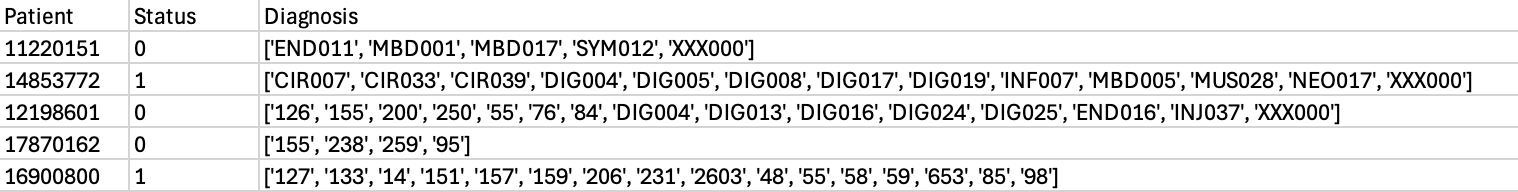
\includegraphics[width=1\textwidth]{snapshot.png}
    \caption{First Five Rows of the Prepared Dataset}
    \label{fig.snapshot}
\end{figure}
\begingroup
\clearpage
\let\clearpage\relax
\vspace*{-16pt}
\chapter[COMPUTATIONAL STUDY]{COMPUTATIONAL STUDY}\label{sec.results}
\endgroup

This chapter presents the computational results for the solution
methods developed in Chapter~\ref{sec.methods}, evaluated on the testbed described in Chapter~\ref{sec.DATAPREP}. The experiments cover
instances sampled from the MIMIC-IV cohort of \numprint{223291}
patients, with cohort sizes ranging from \numprint{1000} to
\numprint{30000} patients. We compare exact combinatorial algorithms,
direct MILP formulations with implementation enhancements, and
variants of the LBBD algorithm. All experiments were conducted on a high-performance compute node with an Intel Xeon Gold 6130F CPU @ 2.10~GHz and 1.5~TB RAM, using Gurobi 12.0.0 as the MILP solver. All algorithms and methods were implemented in Python 3.9.23. A time limit of \numprint{7200} seconds (2 hours) was imposed for all methods, and running times are reported in seconds. Delayed constraint addition is implemented via Gurobi's lazy cut functionality.

The frequency threshold $\ell = 100$ is used throughout, chosen after
preliminary experimentation. In practice, $\ell$ should be set to a
sufficiently large fraction of $|P|$ to ensure statistical reliability
of the mortality rate estimate. As mentioned in Chapter~\ref{sec.probstmnt}, every vertex
$u$ with $|A_u| \le \ell - 1$ and every edge $\{u,v\}$ with
$|A_u \cap A_v| \le \ell - 1$ are removed from the comorbidity graph,
so that $|A_u| \ge \ell$ for each $u \in V$ and
$|A_u \cap A_v| \ge \ell$ for each $\{u,v\} \in E$.

The results are organized as follows. Section~\ref{sec.CCA} compares
the modified Bron--Kerbosch and combinatorial branch-and-bound
algorithms. Section~\ref{sec.milp-dcg} evaluates the two MILP
formulations and their implementation variants.
Section~\ref{sec.lbbds} compares the pure and hybrid LBBD algorithms.
Section~\ref{sec.sidecons} demonstrates the extensibility of the LBBD
framework through a case study incorporating an age-based side
constraint. Section~\ref{sec.exp2-BKscalability} evaluates the
scalability of the modified Bron--Kerbosch algorithm on the full
MIMIC-IV dataset, and Section~\ref{sec.exp3-margMR} presents a
sensitivity analysis and marginal mortality rate experiments. Detailed
results are provided in Appendix~\ref{App.tableDeets}.

The following column headings are used throughout the tables. ``Size''
reports the patient cohort size, and ``No.'' the sample identifier within
a cohort size. ``Clique'' lists the diseases comprising the reported
clique, with disease names abbreviated; full names are provided in
Appendix~\ref{App.Abbs}. ``$\mu$'' denotes the mortality rate of a clique,
and ``Increase'' the percentage by which the mortality rate rises when the
indicated disease or diseases are added to an initial clique. ``Best Obj''
reports the best objective value (mortality rate) found. ``Time'' reports
wall-clock running time rounded down to the nearest second; an entry of
``TO'' indicates that the time limit was reached. ``Gap'' reports the
percentage optimality gap at termination, with zero indicating optimality
within solver tolerance. In LBBD tables, ``\#Opt Cuts'', ``\#Feas Cuts'',
and ``\#CBB Cuts'' report the number of optimality cuts, feasibility cuts,
and CBB cuts added, respectively. In summary tables, ``Avg'' and ``Range''
give the average and the minimum--maximum range across the five samples for
each cohort size.

\section{Comparing Combinatorial Algorithms}\label{sec.CCA}

Table~\ref{tab.SBKCBB} summarizes the results comparing the modified
Bron--Kerbosch algorithm (Algorithm~\ref{alg.BKMMRC}) and the CBB algorithm
(Algorithm~\ref{alg.CBB}). Detailed sample-wise results appear in
Table~\ref{tab.BKCBB} in the appendix. Both methods guarantee
optimality unless the time limit is reached. The column ``\#RC
decrease'' reports the average reduction in recursive calls
attributable to the $\gamma$-upper-bound pruning~\eqref{eq.gammaC}
in the CBB algorithm, which is the primary differentiator between the
two methods.

Both methods solve all tested instances up to \numprint{30000}
patients. For the BK algorithm, average running times increase from
under 1 second for \numprint{1000}-patient instances to approximately
73 seconds for \numprint{30000}-patient instances. The CBB algorithm
is considerably faster: its average running time remains below 1
second for instances with up to \numprint{5000} patients, rises to 1
second at \numprint{10000} patients, 3 seconds at \numprint{15000}
patients, 8 seconds at \numprint{20000} patients, 22 seconds at
\numprint{25000} patients, and 2 seconds at \numprint{30000} patients.
The number of recursive calls grows with instance size for the BK
algorithm, while the CBB algorithm requires far fewer. The average
reduction in recursive calls ranges from 28 for \numprint{1000}-patient
instances to \numprint{1153091} for \numprint{30000}-patient instances.
The average maximum mortality rate across instances ranges from 0.45
at \numprint{1000} patients to 0.97 at \numprint{25000} patients,
with a value of 0.85 at \numprint{30000} patients. The full
\numprint{223291}-patient instance exceeds the time limit for both
algorithms.  
\begin{table}[htpb]
\centering
\resizebox{\textwidth}{!}{\begin{tabular}{rrrrrrrrr}
\toprule
Size & \multicolumn{2}{c}{Best Obj} & \multicolumn{2}{c}{BK, Time} &
\multicolumn{2}{c}{CBB, Time} & \#RC decrease\\
 & Avg & Range & Avg & Range & Avg & Range & Avg \\
\midrule
\numprint{1000} & 0.45 & [0.41, 0.49] & $<1$ & [$<1$, $<1$] & $<1$ &
[$<1$, $<1$] & 28 \\
\numprint{5000} & 0.80 & [0.72, 0.88] & 1 & [1, 1] & $<1$ & [$<1$,
$<1$] & \numprint{2207}\\
\numprint{10000} & 0.86 & [0.81, 0.92] & 2 & [2, 3] & 1 & [1, 1] &
\numprint{20787}\\
\numprint{15000} & 0.95 & [0.89, 1.00] & 8 & [5, 9] & 3 & [2, 4] &
\numprint{89191}\\
\numprint{20000} & 0.97 & [0.96, 0.99] & 24 & [22, 27] & 8 & [7, 8] &
\numprint{241932} \\
\numprint{25000} & 0.97 & [0.97, 0.98] & 47 & [42, 53] & 22 & [20,
26] & \numprint{478683}\\
\numprint{30000} & 0.85 & [0.83, 0.88] & 73 & [66, 83] & 2 & [2, 2] &
\numprint{1153091}\\
\numprint{223291} & UNK\footnotemark & UNK & TO & UNK & UNK & TO & UNK\\
\bottomrule
\end{tabular}}
\caption{\label{tab.SBKCBB} Comparing Modified Bron--Kerbosch and CBB Algorithms}
\end{table}

\footnotetext{UNK stands for Unknown (no value was reported because the run timed out).}

\section{Comparing MILP Solutions}\label{sec.milp-dcg}

We implemented formulation~\eqref{form.milp} using delayed addition of
the linearizing constraints~\eqref{eq.wto0}--\eqref{eq.wtozUB}, which
scale with $|P|$. All violated constraints of this type are added at
BC nodes where an integral solution is encountered as the node LP
relaxation optimum. Preliminary experiments showed this to perform
better than delaying
constraints~\eqref{eq.xyconnectupper-disagg}--\eqref{eq.xyconnectlowerFP}.
We also explored an implementation using an aggregated variant of
constraints~\eqref{eq.xyconnectupper-disagg}, given by
constraint~\eqref{eq.xyconnectupperagg}, in the root LP formulation.
This aggregated form models the requirement as
\begin{align}
    |V \setminus D_i| y_i &\le |V \setminus D_i| - \sum_{j \in V
    \setminus D_i} x_j & \forall i \in P.
    \label{eq.xyconnectupperagg}
\end{align}
Formulation~\eqref{form.CCIP} was implemented using Gurobi's indicator
constraint feature~\citep{gurobi-indicator} for
constraints~\eqref{eq.xlin1CC}--\eqref{eq.xlin3CC}, which model the
products $\bar{x}_u = x_u \cdot t$. These indicator constraints
directly encode the implication that $x_u = 1$ forces $\bar{x}_u = t$
and $x_u = 0$ forces $\bar{x}_u = 0$, without requiring explicit
big-M coefficients. Gurobi internally generates an equivalent MIP
representation during the solution process.
Constraints~\eqref{eq.xyconnectupper-disaggcc}--\eqref{eq.xyconnectlowerFPcc}
are also added in a delayed manner at BC nodes with integral LP optima.

Detailed results comparing formulation~\eqref{form.milp} with
aggregation, formulation~\eqref{form.milp} without aggregation, and
formulation~\eqref{form.CCIP} are reported in Table~\ref{tab.MILPs}
in the appendix. All three formulations solve the
\numprint{1000}-patient instances to optimality: formulation
\eqref{form.milp} with aggregation requires 16--35 seconds per sample,
without aggregation requires 66--75 seconds, and
formulation~\eqref{form.CCIP} requires 2--4 seconds.

Only formulation~\eqref{form.CCIP} consistently solves the
\numprint{5000}-patient instances to optimality. Both variants of
formulation~\eqref{form.milp} reach the time limit with optimality
gaps of 13\%--54\% with aggregation and 13\%--47\% without. For
instances with \numprint{10000} patients or more, all three
formulations reach the time limit on nearly all instances.

\section{Comparing LBBD Variants}\label{sec.lbbds}

In this section, we compare the performance of the two LBBD variants, pure LBBD and hybrid
LBBD. Pure LBBD is the DBC algorithm from
Section~\ref{sec.gamma-lbbd}, using the separation procedure in
Algorithm~\ref{alg.LBBDgamma} at BC nodes where the LP relaxation
optimum is integral. Hybrid LBBD is the algorithm from
Section~\ref{sec.hybridLBBD}, using Algorithm~\ref{alg.hybridLBBD}
instead, and adding CBB cuts at BC nodes where the incumbent
$\ell$-frequent clique contains at least $\tau$ vertices. The root
relaxation is additionally strengthened with CBB cuts generated from
$k$ calls to the CBB algorithm, one for each of the $k$ diseases with
the highest individual mortality rate. Constraint~\eqref{eq.zmuLB} is
updated if a better lower bound is found among the resulting cliques.
Based on preliminary experimentation, we set $\tau = 4$ and $k = 5$
for all experiments.

\begin{table}[htpb]
\centering
\resizebox{\textwidth}{!}{\begin{tabular}{rrrrrrrrr}
 \toprule
Size & \multicolumn{2}{c}{Gap} & \multicolumn{2}{c}{Time} &
\multicolumn{2}{c}{\#Opt Cuts} & \multicolumn{2}{c}{\#Feas Cuts} \\
 & Avg & Range & Avg & Range & Avg & Range & Avg & Range \\
\midrule
\numprint{1000} & 0 & [0, 0] & $<1$ & [$<1$, $<1$] & 13.6 & [4, 21]
& 52.4 & [18, 92]\\
\numprint{5000} & 0 & [0, 0] & 3 & [2, 4] & \numprint{1051} & [783,
\numprint{1365}] & 778.4 & [577, \numprint{1039}]\\
\numprint{10000} & 0 & [0, 0] & 296 & [240, 378] & \numprint{15633} &
[\numprint{11427}, \numprint{19593}] & \numprint{14211} &
[\numprint{12036}, \numprint{16057}]\\
\numprint{15000} & 3 & [0, 6] & TO & [47, TO] & \numprint{60683} &
[\numprint{5010}, \numprint{92190}] & \numprint{52675} &
[\numprint{4452}, \numprint{74083}]\\
\numprint{20000} & 3 & [1, 4] & TO & [TO, TO] & \numprint{72174} &
[\numprint{62069}, \numprint{85761}] & \numprint{72691} &
[\numprint{62164}, \numprint{82328}] \\
\numprint{25000} & 3 & [2, 4] & TO & [TO, TO] & \numprint{65231} &
[\numprint{49369}, \numprint{82039}] & \numprint{76147} &
[\numprint{59438}, \numprint{89502}]\\
\numprint{30000} & 3 & [3, 5] & TO & [TO, TO] & \numprint{61358} &
[\numprint{56441}, \numprint{75841}] & \numprint{137369} &
[\numprint{114797}, \numprint{150718}]\\
\numprint{223291} & 3 & & TO & & \numprint{58825} & & \numprint{42595}
&\\
 \bottomrule
\end{tabular}}
  \caption{\label{tab.SumG} Summary of Results from the Pure LBBD}
\end{table}

\begin{table}[htpb]
 \centering
\resizebox{\textwidth}{!}{\begin{tabular}{rrrrrrrrrrr}
 \toprule
Size & \multicolumn{2}{c}{Gap} & \multicolumn{2}{c}{Time} &
\multicolumn{2}{c}{\#Opt Cuts} & \multicolumn{2}{c}{\#Feas Cuts} &
\multicolumn{2}{c}{\#CBB Cuts}\\
 & Avg & Range & Avg & Range & Avg & Range & Avg & Range & Avg &
 Range\\
\midrule
\numprint{1000} & 0 & [0, 0] & $<1$ & [$<1$, $<1$] & 8.6 & [5, 14] &
0 & [0, 0] & 0 & [0, 0]\\
\numprint{5000} & 0 & [0, 0] & 1 & [1, 2] & \numprint{912} &
[\numprint{736}, \numprint{1249}] & \numprint{566} & [\numprint{507},
\numprint{645}] & 63 & [4, \numprint{183}]\\
\numprint{10000} & 0 & [0, 0] & 100 & [64, \numprint{146}] &
\numprint{9053} & [\numprint{7762}, \numprint{10571}] & \numprint{7062}
& [\numprint{4764}, \numprint{9619}] & \numprint{4599} &
[\numprint{2527}, \numprint{6842}]\\
\numprint{15000} & 0 & [0, 0] & \numprint{1283} & [7, \numprint{2394}]
& \numprint{26169} & [\numprint{577}, \numprint{39564}] & \numprint{4118}
& [45, \numprint{7257}] & \numprint{21731} & [\numprint{189},
\numprint{34797}]\\
\numprint{20000} & 2 & [0, 4] & TO & [TO, TO] & \numprint{81976} &
[\numprint{79347}, \numprint{89610}] & \numprint{72336} &
[\numprint{70127}, \numprint{76794}] & \numprint{44145} &
[\numprint{41677}, \numprint{48648}]\\
\numprint{25000} & 2 & [1, 3] & TO & [TO, TO] & \numprint{74992} &
[\numprint{62595}, \numprint{82335}] & \numprint{76783} &
[\numprint{66641}, \numprint{86002}] & \numprint{43782} &
[\numprint{37470}, \numprint{48200}]\\
\numprint{30000} & 0 & [0, 0] & \numprint{716} & [\numprint{532},
\numprint{1102}] & \numprint{19945} & [\numprint{18620},
\numprint{22737}] & \numprint{24769} & [\numprint{23116},
\numprint{26965}] & \numprint{7158} & [\numprint{6476},
\numprint{8336}]\\
\numprint{223291} & 2 & & TO & & \numprint{423} & & 1 & & 201 &\\
 \bottomrule
\end{tabular}}
\caption{\label{tab.SumH} Summary of Results from the Hybrid LBBD Algorithm}
\end{table}

Tables~\ref{tab.SumG} and~\ref{tab.SumH} summarize the results for
the two LBBD variants; sample-wise details appear in
Tables~\ref{tab.Gam} and~\ref{tab.HybridLBBD} in
Appendix~\ref{App.tableDeets}. Both variants solve the
\numprint{1000}-patient and \numprint{5000}-patient instances quickly:
pure LBBD takes an average of under 1 second and 3 seconds,
respectively, while hybrid LBBD takes under 1 second and 1--2
seconds. On \numprint{10000}-patient instances, both variants solve
all five instances to optimality; hybrid LBBD requires an average of
100 seconds, approximately one third of the 296-second average for
pure LBBD. For \numprint{15000}-patient instances, pure LBBD solves
two instances to optimality (in 47 and \numprint{2278} seconds) and
reaches the time limit on the remaining three with gaps between
0\% and 6\%, while hybrid LBBD solves all five to optimality with an
average of \numprint{1283} seconds.

Both variants reach the time limit on all \numprint{20000}-patient and
\numprint{25000}-patient instances. The pure LBBD reports an average
gap of 3\% at both sizes,
while hybrid LBBD reports an average gap of 2\%. For \numprint{30000}-patient instances, pure LBBD reaches
the time limit on all instances with an average gap of 3\%, while hybrid LBBD solves all five to optimality with an
average of 716 seconds. On the
full \numprint{223291}-patient instance, both variants reach the time
limit; pure LBBD reports a gap of 3\% and hybrid LBBD reports a gap
of 2\%. Overall, the hybrid LBBD algorithm is substantially faster on
instances up to \numprint{15000} patients and is the only method that
solves all \numprint{30000}-patient instances to optimality. Detailed numerical results for all instances and all algorithms are
provided in Appendix~\ref{App.tableDeets}.

\section{Side Constraints and the Hybrid LBBD
Algorithm}\label{sec.sidecons}
An important feature of the LBBD framework is that it is grounded in
integer programming, which allows additional constraints on the $x$
variables to be incorporated into $\calX$ with relative ease. This
contrasts with the CBB algorithm, which may require substantial
modifications to accommodate new constraints. Importantly, the CBB
cut remains valid in the presence of new constraints in $\calX$,
since it still provides a valid upper bound on the optimal solution,
and the hybrid LBBD algorithm continues to be applicable. To
illustrate this, we consider two case studies. In Section~\ref{sec.AgeSide}, an age-based side
constraint is added to the original problem. In Section~\ref{sec.CancerSide}, we incorporate a constraint
requiring the selected clique to contain at least one cancerous
diagnosis, directing the search toward high-mortality clusters
that include cancer as a component.

\subsection{Case Study: Limiting Age-Associated Diseases} \label{sec.AgeSide}

In practice, older patients tend to exhibit more comorbidities and
higher baseline mortality, which can influence the composition of
maximum mortality rate cliques. We define a practical age threshold
of 60, and for each disease $v \in V$ compute the proportion of its
patients who are 60 or older:
\begin{align*}
    a_{60}(v) &\coloneqq \frac{|\{i \in A_v : \text{age}(i) \ge
    60\}|}{|A_v|}, \qquad \forall v \in V.
\end{align*}
We then impose constraint~\eqref{eq.oldagecon}, which limits the
average $a_{60}(v)$ across selected diseases to at most 0.5, with the
aim of identifying high-mortality cliques whose lethality is not
primarily attributable to an older patient composition:
\begin{equation}\label{eq.oldagecon}
    \sum_{v \in V} a_{60}(v) x_v \;\le\; 0.5\,\sum_{v \in V} x_v.
\end{equation}

\begin{figure}[htbp]
    \centering
    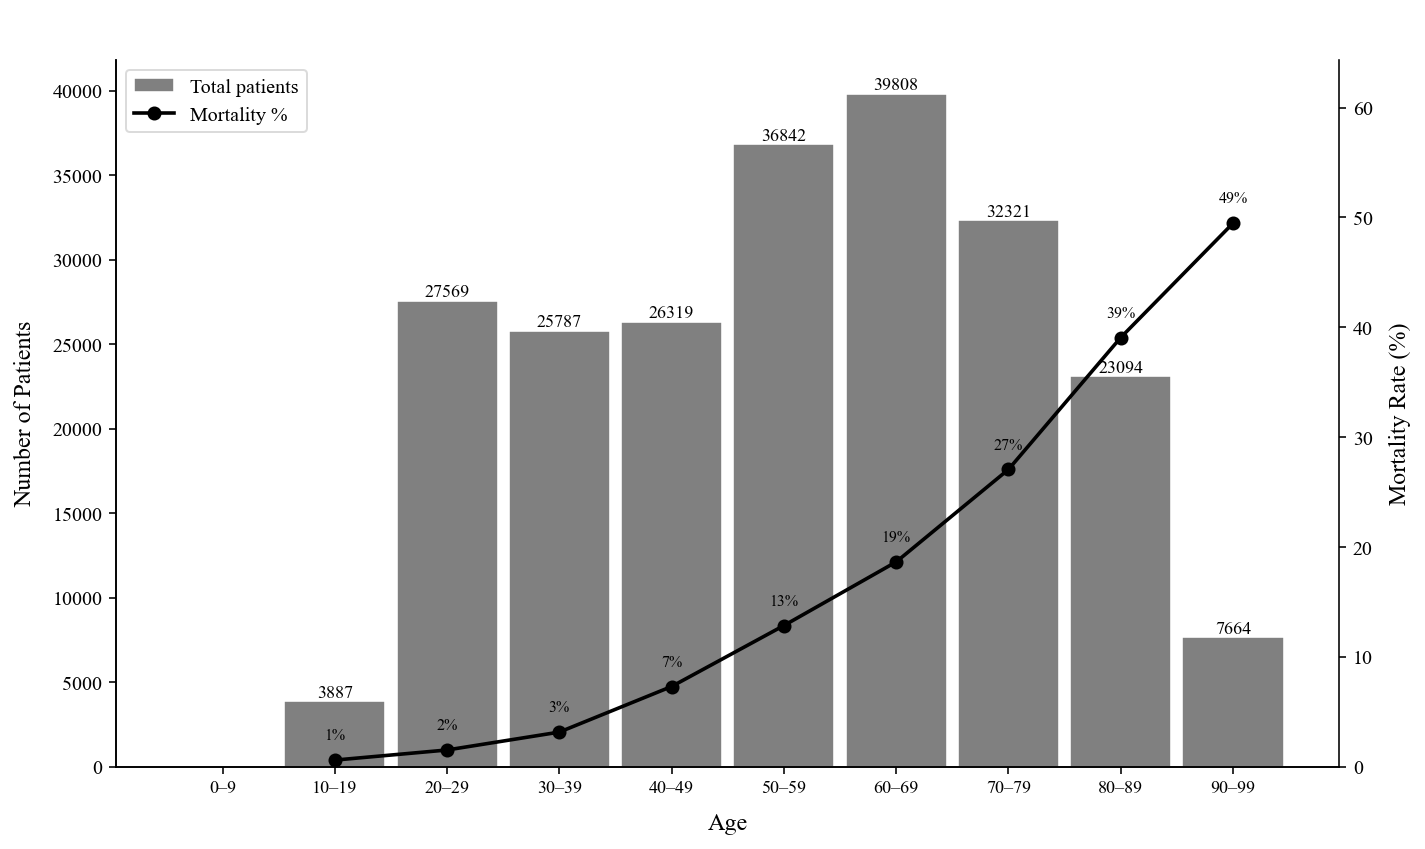
\includegraphics[width=1\textwidth]{hist2.png}
    \caption{Age Distribution and Mortality Rates among Patients in
    Our Dataset}
    \label{fig.age_hist}
\end{figure}

In the dataset, patient ages range from 18 to 91 with an average of
56, and approximately 54\% of patients are younger than 60. Patient
ages are derived from the \texttt{anchor\_age} column in
\texttt{patients.csv}, which caps all ages above 89 at
91~\citep{mimiciv}. Since our threshold of 60 falls below this
ceiling, the cap does not affect the analysis. The age distribution
and mortality rates by age group are shown in
Figure~\ref{fig.age_hist}, using bins
$[0,9],[10,19],\ldots,[80,89],$ $[90,99]$.

We solve problem~\eqref{form.LBBF} with
constraint~\eqref{eq.oldagecon} included in $\calX$ using the hybrid
LBBD algorithm. Constraint~\eqref{eq.zmuLB} is excluded rather than
adjusted, in keeping with our intent to minimize tailoring of the
methodology in the presence of the new constraint.
Table~\ref{tab.Extension} in Appendix~\ref{App.tableDeets} reports
detailed results, summarized in Table~\ref{tab.ExtensionSum}. All
instances across all cohort sizes are solved to optimality.
The addition of this constraint appears to make instances more
tractable compared to the unconstrained results in
Table~\ref{tab.SumH}.

\begin{table}[htbp]
\centering
\resizebox{\textwidth}{!}{\begin{tabular}{rrrrrrrrr}
 \toprule
Size & \multicolumn{2}{c}{Time} & \multicolumn{2}{c}{\#Opt Cuts} &
\multicolumn{2}{c}{\#Feas Cuts} & \multicolumn{2}{c}{\#CBB Cuts}\\
 & Avg & Range & Avg & Range & Avg & Range & Avg & Range\\
\midrule
\numprint{1000} & $<1$ & [$<1$, $<1$] & 5 & [3, 7] & 0 & [0, 0] & 0
& [0, 0]\\
\numprint{5000} & 0 & [0, 1] & 55 & [35, 78] & 34 & [14, 56] & 0 &
[0, 0]\\
\numprint{10000} & 5 & [3, 9] & \numprint{228} & [\numprint{152},
\numprint{273}] & \numprint{189} & [94, \numprint{277}] & 7 & [3,
13]\\
\numprint{15000} & 36 & [12, 45] & \numprint{628} & [\numprint{359},
\numprint{742}] & \numprint{595} & [\numprint{320}, \numprint{769}] &
81 & [27, \numprint{114}]\\
\numprint{20000} & 113 & [89, \numprint{131}] & \numprint{1466} &
[\numprint{1106}, \numprint{1788}] & \numprint{1472} &
[\numprint{948}, \numprint{1921}] & \numprint{290} &
[\numprint{224}, \numprint{350}]\\
\numprint{25000} & \numprint{290} & [\numprint{226}, \numprint{397}] &
\numprint{2724} & [\numprint{2252}, \numprint{3537}] & \numprint{2836}
& [\numprint{2101}, \numprint{3848}] & \numprint{706} &
[\numprint{511}, \numprint{992}]\\
\numprint{30000} & 23 & [18, 29] & \numprint{584} & [\numprint{505},
\numprint{766}] & \numprint{1015} & [\numprint{889},
\numprint{1322}] & 20 & [10, 31]\\
 \bottomrule
\end{tabular}}
  \caption{Summary of Results from the Hybrid LBBD Algorithm with
  Age-Based Side-Constraint}
 \label{tab.ExtensionSum}
\end{table}

Instances with \numprint{15000} patients or fewer are solved in under
one minute. The \numprint{1000}-patient instances are solved in under
1 second using only optimality and feasibility cuts with zero CBB cuts,
and the \numprint{5000}-patient instances in under 1 second on
average. For larger instances, CBB cuts are used more frequently and
running times remain within the time limit, reaching an average of
\numprint{290} seconds at \numprint{25000} patients. For
\numprint{30000}-patient instances, solution times range from 18 to 29
seconds, with an average of 23 seconds.

To examine the effect of the side constraint on the diseases
identified, Tables~\ref{tab.compa6025k} and~\ref{tab.compa6030k}
report the cliques obtained with and without
constraint~\eqref{eq.oldagecon} for the \numprint{25000}-patient and
\numprint{30000}-patient samples, respectively. Results are presented
column-wise for each of the five samples, with ``W/O'' and ``W''
denoting solutions obtained without and with the constraint. Each
table reports the diseases in the clique alongside their
$a_{60}(\cdot)$ values, the mortality rate of the clique, and the
average $a_{60}(\cdot)$ across the clique. Tables~\ref{tab.a60_25k}
and~\ref{tab.a60_30k} in Appendix~\ref{App.tableDeets} summarize the
$a_{60}$ values for all diseases appearing in these tables across the
two cohort sizes. Disease names are abbreviated due to space
limitations; full names are provided in Appendix~\ref{App.Abbs}.

\begin{table}[htbp]
\centering
\resizebox{\textwidth}{!}{
\begin{tabular}{lr|lr|lr|lr|lr|lr|lr|lr|lr|lr}
\toprule
\multicolumn{4}{c|}{Sample \#1} & \multicolumn{4}{c|}{Sample \#2} &
\multicolumn{4}{c|}{Sample \#3} & \multicolumn{4}{c|}{Sample \#4} &
\multicolumn{4}{c}{Sample \#5} \\
\midrule
\multicolumn{2}{c|}{W/O} & \multicolumn{2}{c|}{W} &
\multicolumn{2}{c|}{W/O} & \multicolumn{2}{c|}{W} &
\multicolumn{2}{c|}{W/O} & \multicolumn{2}{c|}{W} &
\multicolumn{2}{c|}{W/O} & \multicolumn{2}{c|}{W} &
\multicolumn{2}{c|}{W/O} & \multicolumn{2}{c}{W} \\
\midrule
Clique & $ a_{60} $ & Clique & $ a_{60} $ & Clique & $ a_{60} $ &
Clique & $ a_{60} $ & Clique & $ a_{60} $ & Clique & $ a_{60} $ &
Clique & $ a_{60} $ & Clique & $ a_{60} $ & Clique & $ a_{60} $ &
Clique & $ a_{60} $ \\
\midrule
OACE & 0.72 & RCU & 0.56 & CA & 0.79 & ONSD & 0.56 & NCD & 0.88 &
PIA & 0.48 & OACE & 0.71 & Hepatitis & 0.28 & SEPT & 0.61 & DCP &
0.58 \\
RF & 0.66 & FevUO & 0.44 & OACE & 0.72 & IntI & 0.54 & OACE & 0.72 &
OLD & 0.47 & HF & 0.79 & OLD & 0.47 & OACE & 0.72 & AlcD & 0.22 \\
PNA & 0.63 & OLD & 0.48 & DLM & 0.73 & MD & 0.38 & AURF & 0.68 & & &
PDX-Unacc & 0.50 & ARenF & 0.71 & DLM & 0.73 & OLD & 0.48 \\
OSNSD & 0.68 & & & RF & 0.66 & & & PDX-Unacc & 0.51 & & & SHK & 0.68
& & & PDX-Unacc & 0.50 & ARenF & 0.71 \\
PDX-Unacc & 0.51 & & & HF & 0.79 & & & OSNSD & 0.67 & & & FED & 0.61
& & & CoagHD & 0.60 & & \\
 &  &  &  & PDX-Unacc & 0.51 &  &  &  &  &  &  &  &  &  &  &  &  &
 &  \\
\midrule
$ \mu $ & Avg & $ \mu $ & Avg & $ \mu $ & Avg & $ \mu $ & Avg & $ \mu
$ & Avg & $ \mu $ & Avg & $ \mu $ & Avg & $ \mu $ & Avg & $ \mu $ &
Avg & $ \mu $ & Avg \\
0.97 & 0.64 & 0.68 & 0.49 & 0.97 & 0.70 & 0.67 & 0.49 & 0.98 & 0.69
& 0.69 & 0.48 & 0.97 & 0.66 & 0.68 & 0.49 & 0.98 & 0.63 & 0.70 &
0.50 \\
\bottomrule
\end{tabular}
}
\caption{Optimal Solutions Found With and Without the Age-Based
Side-Constraint on \numprint{25000}-Patient Samples}
\label{tab.compa6025k}
\end{table}


\begin{table}[htbp]
\centering
\resizebox{\textwidth}{!}{
\begin{tabular}{lr|lr|lr|lr|lr|lr|lr|lr|lr|lr}
\toprule
\multicolumn{4}{c|}{Sample \#1} & \multicolumn{4}{c|}{Sample \#2} &
\multicolumn{4}{c|}{Sample \#3} & \multicolumn{4}{c|}{Sample \#4} &
\multicolumn{4}{c}{Sample \#5} \\
\midrule
\multicolumn{2}{c|}{W/O} & \multicolumn{2}{c|}{W} &
\multicolumn{2}{c|}{W/O} & \multicolumn{2}{c|}{W} &
\multicolumn{2}{c|}{W/O} & \multicolumn{2}{c|}{W} &
\multicolumn{2}{c|}{W/O} & \multicolumn{2}{c|}{W} &
\multicolumn{2}{c|}{W/O} & \multicolumn{2}{c}{W} \\
\midrule
Clique & $ a_{60} $ & Clique & $ a_{60} $ & Clique & $ a_{60} $ &
Clique & $ a_{60} $ & Clique & $ a_{60} $ & Clique & $ a_{60} $ &
Clique & $ a_{60} $ & Clique & $ a_{60} $ & Clique & $ a_{60} $ &
Clique & $ a_{60} $ \\
\midrule
HCSH & 0.79 & RCU & 0.55 & CHF-NH & 0.82 & AlcD & 0.20 & DOA & 0.59
& PS & 0.49 & CardArr & 0.79 & AlcD & 0.21 & HCSH & 0.80 & AlcD &
0.21 \\
ARF  & 0.62 & DOA & 0.59 & DOA    & 0.57 & OLD  & 0.50 & CardArr &
0.79 &      &      & HCSH    & 0.79 & OLD  & 0.51 & SHK  & 0.68 &
OLD  & 0.50 \\
ONSD & 0.56 & AlcD & 0.22 & CUS    & 0.74 &      &      & GD      &
0.59 &      &      & CHF-NH  & 0.82 &      &      & OA   & 0.62 &
&      \\
RCU  & 0.55 &      &      &        &      &      &      & RCU     &
0.57 &      &      & CUS     & 0.73 &      &      &      &      &
&      \\
     &      &      &      &        &      &      &      & CA      &
0.81 &      &      &  &      &      &      &      &      &      &
\\
\midrule
$ \mu $ & Avg & $ \mu $ & Avg & $ \mu $ & Avg & $ \mu $ & Avg & $ \mu
$ & Avg & $ \mu $ & Avg & $ \mu $ & Avg & $ \mu $ & Avg & $ \mu $ &
Avg & $ \mu $ & Avg \\
0.83 & 0.63 & 0.60 & 0.45 & 0.88 & 0.71 & 0.65 & 0.35 & 0.87 & 0.67
& 0.61 & 0.49 & 0.84 & 0.78 & 0.66 & 0.36 & 0.85 & 0.70 & 0.64 &
0.36 \\
\bottomrule
\end{tabular}
}
\caption{Optimal Solutions Found With and Without the Age-Based
Side-Constraint on \numprint{30000}-Patient Samples}
\label{tab.compa6030k}
\end{table}

The solutions obtained without the side constraint show a consistent
pattern: every disease in these cliques has $a_{60}(v) \ge 0.5$,
meaning the majority of its patients are aged 60 or older. For the
\numprint{25000}-patient instances, diseases appearing in the optimal
cliques include neurocognitive disorders ($a_{60} = 0.88$), congestive
heart failure ($a_{60} = 0.79$), coronary atherosclerosis
($a_{60} = 0.79$), disorders of lipid metabolism ($a_{60} = 0.73$),
and other aftercare encounters ($a_{60} = 0.72$). The
\numprint{30000}-patient instances show a similar pattern, with
congestive heart failure ($a_{60} = 0.82$), coronary atherosclerosis
($a_{60} = 0.81$), hypertension with complications ($a_{60} = 0.80$),
and cardiac arrhythmia ($a_{60} = 0.79$) appearing prominently. The
average $a_{60}(\cdot)$ across clique diseases exceeds 0.6 in all
instances, with mortality rates in the range $[0.97, 0.98]$ for the
\numprint{25000}-patient instances and $[0.83, 0.88]$ for the
\numprint{30000}-patient instances, consistent with the values in
Tables~\ref{tab.compa6025k} and~\ref{tab.compa6030k}. These results
indicate that, without the side constraint, the optimal cliques may
reflect the elevated baseline mortality of older patients as much as
the synergistic lethality of co-occurring diseases.

The solutions obtained with the side constraint incorporate diseases
with lower $a_{60}(\cdot)$ values, including alcohol-related disorders
($a_{60} = 0.22$), hepatitis ($a_{60} = 0.28$), mood disorders
($a_{60} = 0.38$), and fever of unknown origin ($a_{60} = 0.44$, as
in Sample~\#1 of Table~\ref{tab.compa6025k}). Mortality rates remain
relatively high at $[0.67, 0.70]$ for the \numprint{25000}-patient
instances and $[0.60, 0.66]$ for the \numprint{30000}-patient
instances. In the presence of the age-based constraint, the
high-mortality cliques frequently include alcohol-related disorders,
other liver diseases, and acute renal failure, consistent with
clinical observations that alcohol-related liver disease co-occurring
with acute kidney injury is associated with elevated short-term
mortality across adult age ranges~\citep{altamirano2012acute}.

\subsection{Case Study: Finding Cancer-Containing
Cliques}\label{sec.CancerSide}

Cancer is among the leading causes of mortality worldwide and
represents a major driver of inpatient mortality in the United
States~\citep{Xu2016}. Within the MIMIC-IV dataset, approximately
20\% of the full cohort, \numprint{44175} of \numprint{223291}
patients, carry at least one cancerous diagnosis, making cancer a
clinically prominent component of the comorbidity landscape. As
illustrated in Figure~\ref{fig.cancer_bar}, the ten most prevalent
cancer diagnoses in the dataset vary substantially in both frequency
and individual mortality rate, with secondary malignancies (SM) and
conditions due to neoplasm or its treatment (CNTN) among the most
lethal. Understanding which non-cancerous diseases co-occur with
cancer to produce the highest joint mortality rates is therefore of
direct clinical relevance for risk stratification and proactive care
planning~\citep{Earle2008, Numico2015}.

\begin{figure}[htbp]
    \centering
    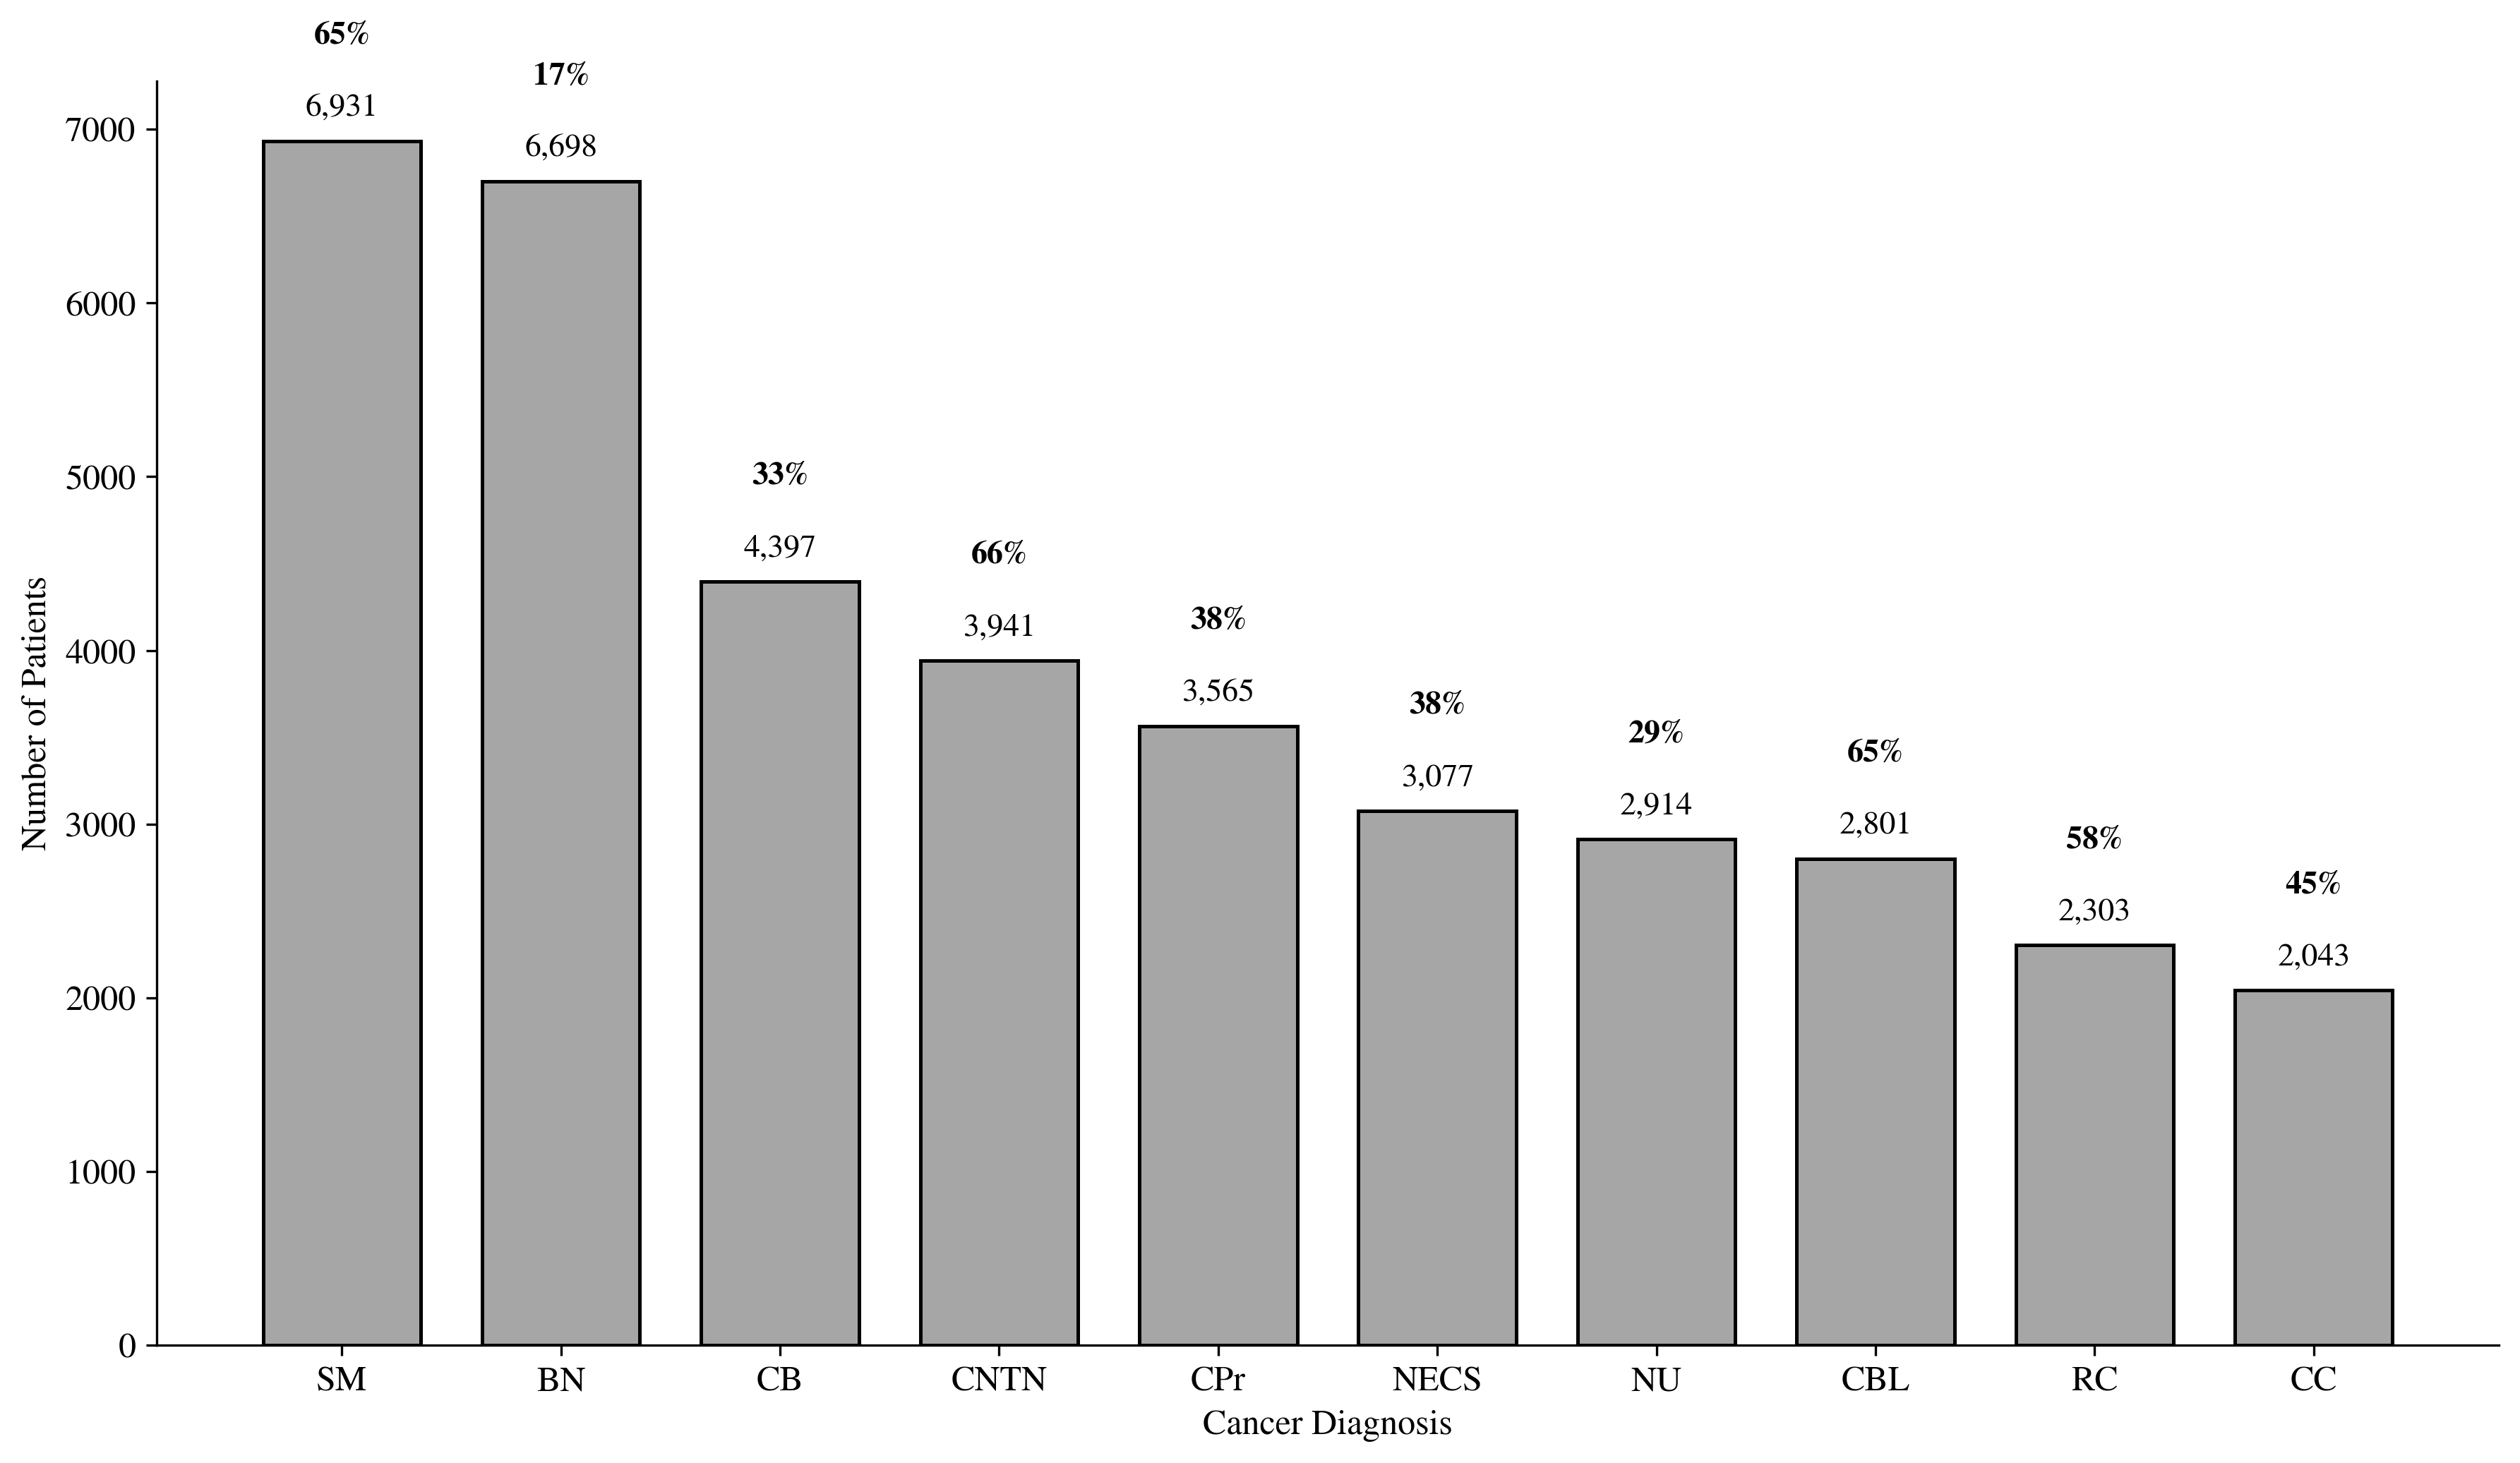
\includegraphics[width=1\textwidth]{top_10_cancers.png}
    \caption{Top-10 Cancer Diagnoses and Their Mortality Rates among
    Patients in Our Dataset}
    \label{fig.cancer_bar}
\end{figure}

We denote by $T$ the set of CCS and CCSR codes corresponding to any
cancerous diagnosis. To identify high-mortality cliques that include
at least one cancer diagnosis, we incorporate the following constraint
into $\calX$:
\begin{equation}\label{eq.Cancon}
    \sum_{v \in T} x_v \;\ge\; 1.
\end{equation}
Constraint~\eqref{eq.zmuLB} is excluded rather than adjusted, in
keeping with our intent to minimize tailoring of the methodology in
the presence of the new constraint. We solve the resulting problem
using the hybrid LBBD algorithm.

Table~\ref{tab.CancerExtension}
summarizes the results across the remaining cohort sizes; detailed
sample-wise results are provided in Table~\ref{tab.cancer_cliques} in
Appendix~\ref{App.tableDeets}. Instances with \numprint{1000} patients are excluded from this case since all five random samples contain no patient carrying a cancerous diagnosis, rendering constraint~\eqref{eq.Cancon} infeasible. 

\begin{table}[htbp]
\centering
\resizebox{\textwidth}{!}{
\begin{tabular}{rrrrrrrrr}
\toprule
Size & \multicolumn{2}{c}{Time} & \multicolumn{2}{c}{\#Opt Cuts} &
\multicolumn{2}{c}{\#Feas Cuts} & \multicolumn{2}{c}{\#CBB Cuts}\\
 & Avg & Range & Avg & Range & Avg & Range & Avg & Range\\
\midrule
\numprint{5000}
& $<1$
& [$<1$, $<1$]
& \numprint{2}
& [\numprint{1}, \numprint{3}]
& \numprint{0}
& [\numprint{0}, \numprint{0}]
& \numprint{0}
& [\numprint{0}, \numprint{0}] \\
\numprint{10000}
& $<1$
& [$<1$, \numprint{1}]
& \numprint{6}
& [\numprint{0}, \numprint{14}]
& \numprint{4}
& [\numprint{0}, \numprint{19}]
& \numprint{0}
& [\numprint{0}, \numprint{0}] \\
\numprint{15000}
& \numprint{2}
& [\numprint{1}, \numprint{2}]
& \numprint{45}
& [\numprint{17}, \numprint{79}]
& \numprint{79}
& [\numprint{4}, \numprint{166}]
& \numprint{0}
& [\numprint{0}, \numprint{0}] \\
\numprint{20000}
& \numprint{29}
& [\numprint{20}, \numprint{42}]
& \numprint{247}
& [\numprint{161}, \numprint{308}]
& \numprint{541}
& [\numprint{360}, \numprint{630}]
& \numprint{13}
& [\numprint{5}, \numprint{26}] \\
\numprint{25000}
& \numprint{61}
& [\numprint{45}, \numprint{78}]
& \numprint{585}
& [\numprint{361}, \numprint{751}]
& \numprint{1087}
& [\numprint{740}, \numprint{1369}]
& \numprint{84}
& [\numprint{40}, \numprint{126}] \\
\numprint{30000}
& \numprint{84}
& [\numprint{65}, \numprint{96}]
& \numprint{1105}
& [\numprint{752}, \numprint{1264}]
& \numprint{1927}
& [\numprint{1420}, \numprint{2199}]
& \numprint{198}
& [\numprint{110}, \numprint{276}] \\
\numprint{223291}
& \numprint{419}
&
& \numprint{1278}
&
& \numprint{41}
&
& \numprint{994}
&  \\
\bottomrule
\end{tabular}}
  \caption{Summary of Results from the Hybrid LBBD Algorithm with
  Cancer-Containing Side-Constraint}
\label{tab.CancerExtensionSum}
\end{table}

In Table~\ref{tab.CancerExtensionSum}, all instances are solved to optimality (0\% gap). The cancer
constraint makes the problem more tractable than the
unconstrained case: the complete dataset that required hundreds of seconds under
the hybrid LBBD without any side constraint (Table~\ref{tab.SumH})
is solved here in a fraction of that time. For cohort sizes up to
\numprint{15000} patients, all instances are solved in under 2
seconds with no CBB cuts required, indicating that the constraint
alone guides the search effectively. CBB cuts begin to contribute at
\numprint{20000} patients (average 13 cuts) and play an increasingly
important role at larger sizes, reaching an average of 198 cuts at
\numprint{30000} patients and 994 cuts on the full
\numprint{223291}-patient instance. The number of optimality and
feasibility cuts grows steadily with cohort size, peaking at averages
of \numprint{1105} and \numprint{1927}, respectively, at
\numprint{30000} patients, before dropping substantially on the full
dataset where the CBB cuts shoulder more of the pruning burden.

To further explore cancer-containing cliques in the complete dataset, we fix exactly one
cancer diagnosis and identify the combination of additional diseases
that maximizes the mortality rate of the resulting clique. We
substitute constraint~\eqref{eq.Cancon} with:
\begin{equation}\label{eq.CanFixcon}
    \sum_{v \in T_{10}} x_v \;=\; 1,
\end{equation}
where $T_{10} = \{\text{SM, BN, CB, CNTN, CPr, NECS, NU, CBL, RC, CC}\}$
denotes the set of the ten most prevalent cancer diagnoses in the
dataset (Figure~\ref{fig.cancer_bar}). For each cancer diagnosis
$C^0 $ from $T_{10}$, we solve problem~\eqref{form.LBBF} with
constraint~\eqref{eq.CanFixcon} and $x_{C^0} = 1$ fixed, effectively
initializing the hybrid LBBD with $C^0$ as the seed clique and
identifying the optimal set of additional diseases $U$ to combine
with it.

\begin{table}[htbp]
\centering
\resizebox{\textwidth}{!}{%
\begin{tabular}{lclcrr}
\toprule
{$C^0$} & \multicolumn{1}{c}{{$\mu(C^0)$}} & {Additional
diseases $U$} & {$\mu(C^0 \cup U)$} & {Increase} & Time\\
\midrule
\multirow{1}{*}{SM} & 0.65 & AURF, CNTN, DLM, OACE, RF, OSS, FED &
1.00 & 54\% & 218 \\
\multirow{1}{*}{BN} & 0.18 & OSNSD, AA, CKD, Hypo, DLM, CoagHD &
0.74 & 331\% & 206 \\
\multirow{1}{*}{CB} & 0.33 & RCU, EsHyp, ONSD, SM, FD & 0.83 &
152\% & 10 \\
\multirow{1}{*}{CNTN} & 0.67 & DLM, SEPT, AURF, AFRD, OACE & 1.00 &
51\% & 135 \\
\multirow{1}{*}{CPr} & 0.38 & CardArr, RCU, GSID, OA, DOA, ARenF &
0.80 & 113\% & 10 \\
\multirow{1}{*}{NECS} & 0.38 & ARenF, CardArr, DOA, FD, RCU, EsHyp,
E-AMD, DLM & 0.86 & 128\% & 27 \\
\multirow{1}{*}{NU} & 0.46 &  & 0.46 & 0\% & 8 \\
\multirow{1}{*}{CBL} & 0.65 & ARF, CardArr, DLM, SM & 0.96 & 48\% &
14 \\
\multirow{1}{*}{RC} & 0.58 & RF, OACE, DLM, PNA & 0.97 & 67\% & 9 \\
\multirow{1}{*}{CC} & 0.45 & GD, SM, RCU & 0.70 & 56\% & 8 \\
\bottomrule
\end{tabular}%
}
\caption{Optimal Cancer-Anchored Cliques Formed by the Addition of
Other Diseases}
\label{tab.cancer_fixed}
\end{table}

Table~\ref{tab.cancer_fixed} reports the results. The individual
mortality rates of the ten cancer diagnoses vary considerably, from
0.18 for benign neoplasms (BN) to 0.67 for conditions due to neoplasm
or its treatment (CNTN), reflecting the well-documented heterogeneity
in prognosis across cancer types~\citep{Earle2008}. The percentage
increase in mortality rate upon adding extra diseases is
inversely related to the baseline cancer mortality: cancers with low
individual mortality (BN at 0.18, CB at 0.33) exhibit the largest
relative gains (331\% and 152\%, respectively), while high-mortality
cancers (CNTN at 0.67, SM at 0.65) show more modest increases (51\%
and 54\%). This pattern suggests that the co-occurring diseases
identified for low-mortality cancers are particularly strong mortality
drivers in combination, rather than independently.

Secondary malignancies (SM) and disorders of lipid metabolism (DLM)
appear as additional diseases across multiple cancer anchors,
suggesting they act as broad comorbidity amplifiers regardless of the
primary cancer type. The co-occurrence of SM with acute and
unspecified renal failure (AURF) and respiratory failure (RF) in the
SM-anchored clique is consistent with the elevated short-term
mortality observed in patients with multi-organ involvement in
advanced malignancy~\citep{Numico2015, Charlson1987}. Similarly, the
combination of CNTN with septicemia (SEPT) and AURF reflects the
well-documented vulnerability of oncology patients to infectious
complications and organ failure during active
treatment~\citep{Kuderer2011}. Respiratory cancers (RC) paired with
respiratory failure (RF), pneumonia (PNA), disorders of lipid
metabolism (DLM), and other aftercare encounters (OACE) reach a
mortality rate of 0.97, consistent with the poor prognosis associated
with advanced lung disease and systemic
compromise~\citep{Niederman2022}.

The SM-anchored and CNTN-anchored cliques both achieve a mortality
rate of 1.00, meaning every patient in the dataset simultaneously
carrying all diseases in these cliques is recorded as expired. While
this reflects the extreme severity of these combinations in the
MIMIC-IV cohort, it should be interpreted cautiously. The
$\ell$-frequency requirement ensures these cliques are supported by
at least $\ell = 100$ patients in the \numprint{223291}-patient
dataset, lending statistical credibility to the finding.

The results of this case study further demonstrate that the hybrid
LBBD framework accommodates cancer-specific constraints without
modification to the core algorithm, and that the resulting
formulation remains tractable across all tested cohort sizes. Full
disease names for all abbreviations used in
Table~\ref{tab.cancer_fixed} are provided in
Appendix~\ref{App.Abbs}.

The results of these two case studies illustrate that the hybrid LBBD framework accommodates side constraints without modification to the core algorithm, and that the resulting formulation remains tractable in practice.

Having established the LBBD framework's flexibility and scalability via decomposition, we now turn to a complementary enumeration-based analysis of small, highly lethal cliques on the full cohort.

\section{Enumeration and Exploring the Comorbidity
Graph}\label{sec.exp2-BKscalability-intro}

The unrestricted MMRCP~\eqref{eq.MMRCP} introduced in Chapter~\ref{sec.probstmnt}
imposes no bound on clique size, reflecting applications in medical
research where restricting attention to small cliques may fail to
capture broader interactions among comorbid diseases that jointly
influence patient outcomes. Alternatively, we can seek an $\ell$-frequent clique of size at most $b$ in the comorbidity
graph $G$ that maximizes the mortality rate. This version focuses
on small but highly lethal disease clusters, which are of particular
value to clinicians assessing future mortality risk in patients with
multiple comorbidities. 

Given a positive integer $b$, the size-restricted problem seeks an
$\ell$-frequent clique $C$ in $G$ with at most $b$ diseases maximizing
$\mu(C)$:
\begin{equation}
    \label{eq.MRP}
    \max\left\{\mu(C) : C \text{ is a nonempty $\ell$-frequent
    clique in } G,\ |C| \le b\right\}.
\end{equation}
The upper bound $b$ ensures that identified clusters are small, as
smaller clusters tend to carry greater diagnostic significance. It is
generally the case that patients with a large number of comorbidities
have higher mortality rates, so restricting $b$ guards against
trivially large cliques driven by that effect. The lower bound $\ell$
ensures that the mortality rate $\mu(C)$ is a statistically reliable
estimate.

A natural variant of problem~\eqref{eq.MRP} is the \textit{maximum
marginal mortality rate clique problem}. Given a pre-established clique
$C^0$ of strictly fewer than $b$ diseases, we seek at most $b -
|C^0|$ additional diseases that maintain the clique property when
added to $C^0$ and maximize the mortality rate of the resulting clique:
\begin{equation}
    \label{eq.margMRP}
    \max\left\{\mu(C) : C \text{ is a nonempty $\ell$-frequent
    clique in } G,\ C \supseteq C^0,\ |C| \le b \right\}.
\end{equation}
This formulation enhances the prognostic potential of the methodology
for patient populations already carrying known diagnoses.
Problem~\eqref{eq.MRP} is a special case of~\eqref{eq.margMRP}
obtained by setting $C^0 = \emptyset$, and both are special cases of
MMRCP~\eqref{eq.MMRCP}.

Algorithm~\ref{alg.MargBKMMRC} in Appendix~\ref{App.Pseudos} solves
both problems~\eqref{eq.MRP} and~\eqref{eq.margMRP} by adapting
the modified BK algorithm (Algorithm~\ref{alg.BKMMRC}) of Section~\ref{sec.MBK} with two changes.
First, the recursion also terminates when $|C| = b$, enforcing the
size bound. Second, rather than tracking a single incumbent, the
algorithm maintains a global max-heap $Q$ prioritized by mortality
rate, into which every $\ell$-frequent clique encountered is inserted.
This allows the top-$K$ highest-mortality cliques to be retrieved for
any positive integer $K$. If $C^0$ is nonempty, it is inserted into
$Q$ initially and the candidate set $L$ is initialized to the common
neighbors of all vertices in $C^0$; otherwise $L = V$. The set
$\texttt{Den}$, representing $\bigcap_{u \in C} A_u$, is tracked
incrementally as in Section~\ref{sec.MBK} to avoid redundant
recomputation.

\subsection{Size-Restricted Most Lethal Cliques}\label{sec.exp2-BKscalability}

The goal of this section is to address problem~\eqref{eq.MRP} and evaluate the performance of the
modified BK algorithm on the complete MIMIC-IV dataset of
\numprint{223291} patient records, which represents the scale at which
the problem is most relevant in practice. Table~\ref{tab.mimicXBK}
presents results for this full dataset. Column ``\#Dec'' records the
number of deceased patients (the numerator of the mortality rate) for
reference, and column ``\#RC'' records the number of recursive calls.
For each value of $b$, we report the top-5 most lethal cliques.

\begin{table}[htbp]
    \small \centering
    {\begin{tabular}{clrrrr}
     \toprule
          $b$ & Clique & \#Dec & $\mu$ & Time & \#RC\\
          \midrule
         \multirow{5}{*}{1} & OACE & \numprint{184636} & 0.83 &
         \multirow{5}{*}{\numprint{1}} &
         \multirow{5}{*}{\numprint{623}} \\
          & CP & \numprint{172829} & 0.77 & & \\
          & GCb & \numprint{165264} & 0.74 & & \\
          & MNWo & \numprint{161972} & 0.73 & & \\
          & ECP & \numprint{156766} & 0.70 & & \\
\midrule
     \multirow{5}{*}{2} & ECP, OACE & \numprint{211396} & 0.95 &
     \multirow{5}{*}{\numprint{4}} &
     \multirow{5}{*}{\numprint{9148}} \\
          & HepF, OACE & \numprint{210706} & 0.94 & & \\
          & AHCD, OACE & \numprint{207341} & 0.93 & & \\
          & SHK, OACE & \numprint{206481} & 0.92 & & \\
          & Coma, OACE & \numprint{206079} & 0.92 & & \\
\midrule
     \multirow{5}{*}{3} & ECP, CNTN, OACE & \numprint{214515} & 0.96 &
     \multirow{5}{*}{\numprint{24}} &
     \multirow{5}{*}{\numprint{136080}} \\
          & ECP, SM, OACE & \numprint{213829} & 0.96 & & \\
          & SHK, HepF, OACE & \numprint{213511} & 0.96 & & \\
          & CD, HepF, OACE & \numprint{213124} & 0.95 & & \\
          & RF, HepF, OACE & \numprint{213076} & 0.95 & & \\
\midrule
     \multirow{5}{*}{4} & SHK, HepF, UTI, OACE & \numprint{218016} &
     0.98 & \multirow{5}{*}{\numprint{119}} &
     \multirow{5}{*}{\numprint{1570449}} \\
          & CD, HepF, UTI, OACE & \numprint{217156} & 0.97 & & \\
          & HP, AMI, OACE, DMWC & \numprint{216818} & 0.97 & & \\
          & HF, HepF, OACE, PNA & \numprint{216799} & 0.97 & & \\
          & HF, Hypo, HepF, OACE & \numprint{216524} & 0.97 & & \\
         \bottomrule
    \end{tabular}}
        \caption{Top-5 Most Lethal Cliques in the \numprint{223291}-Patient
    Dataset Found by Algorithm~\ref{alg.MargBKMMRC}}
    \label{tab.mimicXBK}
\end{table}

Algorithm~\ref{alg.MargBKMMRC} handles the full dataset efficiently across
all values of $b$. Running time grows from 1 second at $b=1$ to 119
seconds at $b=4$, while the number of recursive calls grows from 623
to over 1.5 million, reflecting the increasing combinatorial
complexity with clique size. Among individual diseases ($b=1$), other
aftercare encounter (OACE) has the highest mortality rate at 0.83,
followed by cancer of pancreas (CP) at 0.77 and gastrointestinal
cancers of the bile duct (GCb) at 0.74. As expected, the maximum
mortality rate increases with $b$. At $b=2$, pairing ECP with OACE
yields a rate of 0.95; at $b=3$, the triple \{ECP, CNTN, OACE\}
reaches 0.96; and at $b=4$, the combination \{SHK, HepF, UTI, OACE\}
attains 0.98. The persistent appearance of OACE across all clique
sizes at $b \ge 2$ reflects its frequent co-occurrence with severe
inpatient conditions in the MIMIC-IV dataset. The high mortality rates
associated with hepatic failure (HepF) in combination with shock (SHK)
or cardiac dysrhythmias (CD) are consistent with clinical observations
of poor prognosis in patients with acute-on-chronic liver failure and
hemodynamic instability~\citep{Hernaez2017,Moreau2013}. The recurrence
of cancer-related groups (ECP, CNTN, SM) is in line with elevated
short-term mortality documented in oncology inpatients with advanced
disease~\citep{Earle2008,Numico2015}.

To explore a broader set of disease interactions, we remove from the
\numprint{223291}-patient dataset every patient diagnosed with hepatic
failure (HepF) or other aftercare encounters (OACE), the two conditions
most dominant in Table~\ref{tab.mimicXBK}. The resulting cohort of
\numprint{211391} patients is analyzed using Algorithm~\ref{alg.MargBKMMRC},
and results are reported in Table~\ref{tab.mimicXBKdeletion}.

\begin{table}[htbp]
    \small \centering
    {\begin{tabular}{clrrrr}
          \toprule
         $b$ & Clique & \#Dec & $\mu$ & Time& \#RC\\[0.5ex]
          \midrule
         \multirow{5}{*}{1} & CP & \numprint{163619} & 0.77 &
         \multirow{5}{*}{\numprint{1}} &
         \multirow{5}{*}{\numprint{621}} \\
          & GCb & \numprint{156457} & 0.74 & & \\
          & MNWo & \numprint{153340} & 0.73 & & \\
          & ECP & \numprint{148411} & 0.70 & & \\
          & SM & \numprint{147450} & 0.70 & & \\
\midrule
     \multirow{5}{*}{2} & CAVF, Coma & \numprint{187321} & 0.89 &
     \multirow{5}{*}{\numprint{4}} &
     \multirow{5}{*}{\numprint{9018}} \\
          & ARF, SM & \numprint{180327} & 0.85 & & \\
          & ECP, CNTN & \numprint{179863} & 0.85 & & \\
          & ECP, SM & \numprint{176676} & 0.84 & & \\
          & RF, SM & \numprint{176562} & 0.84 & & \\
\midrule
     \multirow{5}{*}{3} & SM, ARF, PHD & \numprint{192554} & 0.91 &
     \multirow{5}{*}{\numprint{23}} &
     \multirow{5}{*}{\numprint{132907}} \\
          & RF, CNTN, SM & \numprint{190924} & 0.90 & & \\
          & ARF, SM, Phleb & \numprint{190876} & 0.90 & & \\
          & SM, ND, PHD & \numprint{190640} & 0.90 & & \\
          & CAVF, Coma, RF & \numprint{190251} & 0.90 & & \\
\midrule
      \multirow{5}{*}{4} & SHMSA, SM, ARF, PHD & \numprint{199754} &
      0.94 & \multirow{5}{*}{\numprint{118}} &
      \multirow{5}{*}{\numprint{1523191}} \\
          & RC, CNTN, RF, DLM & \numprint{199739} & 0.94 & & \\
          & ARF, SHMSA, SM, Phleb & \numprint{199647} & 0.94 & & \\
          & InjE, SM, DMWC, ARF & \numprint{199647} & 0.94 & & \\
          & CoagHD, NV, PNA, SM & \numprint{198850} & 0.94 & & \\
         \bottomrule
    \end{tabular}}
        \caption{Top-5 Most Lethal Cliques in the \numprint{211391}-Patient
    Dataset Found by Algorithm~\ref{alg.MargBKMMRC}}
    \label{tab.mimicXBKdeletion}
\end{table}

After the exclusion, cancer of pancreas (CP) carries the highest
individual mortality rate at 0.77, followed by GCb at 0.74 and MNWo
at 0.73, the same top three as in Table~\ref{tab.mimicXBK} after
removing OACE. At $b=2$, the pair \{CAVF, Coma\} achieves the highest
pairwise rate of 0.89. Secondary malignancies (SM) feature prominently
across $b \in \{2,3,4\}$, appearing in the majority of top cliques at
each level. At $b=3$, the triple \{SM, ARF, PHD\} reaches 0.91 in 23
seconds with \numprint{132907} recursive calls, and at $b=4$, four of
the five top cliques achieve 0.94 in 118 seconds. Notably, \{SHMSA,
SM, ARF, PHD\} and \{RC, CNTN, RF, DLM\}, the latter involving
respiratory cancers, cancer treatment-related conditions, respiratory
failure, and lipid metabolism disorders, both attain 0.94. The
frequent co-occurrence of SM with pulmonary and hematologic conditions
is consistent with the elevated mortality observed in patients with
multi-organ involvement in advanced
malignancy~\citep{Earle2008,Numico2015,Charlson1987}. The combination
of respiratory cancers with respiratory failure and metabolic
derangement reflects well-documented interactions between advanced
cancer and systemic compromise~\citep{Niederman2022}.

Analyzing the dataset after removing the dominant conditions from
Table~\ref{tab.mimicXBK} reveals a qualitatively different set of
lethal comorbidity patterns, illustrating how the framework can be
used to investigate lesser-known disease combinations. The rapid
escalation of mortality rates with increasing clique size, even among
diseases not individually recognized as acutely lethal, underscores
the value of a systematic comorbidity-aware approach.

\subsection{Marginal Mortality Rate Analysis}\label{sec.exp3-margMR}

The experiments in this section focus on problem~\eqref{eq.margMRP}
with a nonempty $C^0$, using the \numprint{211391}-patient dataset
from Section~\ref{sec.exp2-BKscalability}. For each value of $b$, we
set $C^0$ to be the fifth highest mortality rate clique from
Table~\ref{tab.mimicXBKdeletion}: $C^0 = \{\text{SM}\}$ for $b=1$,
$C^0 = \{\text{RF, SM}\}$ for $b=2$, $C^0 = \{\text{CAVF, Coma,
RF}\}$ for $b=3$, and $C^0 = \{\text{CoagHD, NV, PNA, SM}\}$ for
$b=4$. The results in
Tables~\ref{tab.mimicXBK} and~\ref{tab.mimicXBKdeletion} already
exhibit containment relationships among the top cliques as $b$
increases, so fixing $C^0$ in this way directs the search toward
high marginal mortality cliques not immediately visible from those
tables.

Two experiments are conducted for each $C^0$. In the first,
for each $u \in V \setminus C^0$, we compute $\mu(C^0 \cup
\{u\})$ without requiring $C^0 \cup \{u\}$ to be a clique,
and return the top results by highest marginal mortality rate.
In the second, Algorithm~\ref{alg.MargBKMMRC} is used to find
the highest marginal mortality rate \textit{cliques} containing
$C^0$, allowing the addition of one and then two more diseases.

\begin{table}[htbp]
\centering
\resizebox{\textwidth}{!}{%
\begin{tabular}{lclcrr}
\toprule
{Initial clique $C^0$} & \multicolumn{1}{c}{{$\mu(C^0)$}} & {Additional
disease $u$} & {$\mu(C^0 \cup \{u\})$} & {Increase} & Cluster
type\\
\midrule
\multirow{5}{*}{SM} & 0.70 & Coma & 0.87 & 25\% & 1-defective
clique \\
 & 0.70 & APV & 0.86 & 24\% & 1-defective clique \\
 & 0.70 & CUS & 0.86 & 23\% & 1-defective clique \\
 & 0.70 & ARF & 0.85 & 22\% & clique \\
 & 0.70 & SHK & 0.85 & 21\% & 1-defective clique \\
\midrule
\multirow{5}{*}{RF, SM} & 0.84 & ECP & 0.95 & 13\% & 1-defective
clique\\
 & 0.84 & DOA & 0.92 & 11\% & 2-defective clique \\
 & 0.84 & OLRD & 0.92 & 10\% & 2-defective clique \\
 & 0.84 & DSD & 0.91 & 9\% & 1-defective clique \\
 & 0.84 & PF & 0.91 & 9\% & 1-defective clique \\
\midrule
\multirow{3}{*}{CAVF, Coma, RF} & 0.90 & AURF & 0.91 & 1\% &
1-defective clique\\
 & 0.90 & FED & 0.91 & 1\% & clique \\
 & 0.90 & PDX-Unacc & 0.90 & -1\% & 2-defective clique \\
\midrule
\multirow{2}{*}{CoagHD, NV, PNA, SM} & 0.94 & FED & 0.94 & 1\% &
clique \\
 & 0.94 & PDX-Unacc & 0.94 & 0\% & clique \\[3pt]
\bottomrule
\end{tabular}%
}
\caption{Top-3 Most Lethal Subsets Formed by the Addition of a Single
Disease}
\label{tab.margMRplus1SA}
\end{table}

Table~\ref{tab.margMRplus1SA} reports the results of the first experiment. For each $C^0$, the table lists the additional disease
$u$ yielding the highest, second highest, and third highest increase
in mortality rate, along with the percentage by which
$\mu(C^0 \cup \{u\})$ exceeds $\mu(C^0)$.

When $C^0$ is small, the addition of a single disease can produce
substantial gains. Adding coma to \{SM\} raises the mortality rate
from 0.70 to 0.87 (a 25\% increase), while adding aspiration
pneumonitis (APV) yields 24\%. By contrast, when $|C^0|$ is larger
and $\mu(C^0)$ is already high, marginal gains diminish. For
$C^0 = \{\text{CoagHD, NV, PNA, SM}\}$ with $\mu(C^0) = 0.94$,
addition of FED increases the mortality rate by 1\%.

The column ``Cluster type'' characterizes each subset using the notion
of a \textit{$k$-defective clique}: a vertex set $S \subset V$ is $k$-defective
if the induced subgraph $G[S]$ contains at least $\binom{|S|}{2} - k$
edges, i.e., it falls short of a complete graph by at most $k$ edges.
A standard clique is 0-defective. This characterization is used here
as a natural way to describe near-clique structure; alternative
relaxations such as $k$-plexes~\citep{BBSBIVH11kplex} or
$\gamma$-quasi-cliques~\citep{Pattillo2013qclique} could also be
applied with suitable parameter choices. Three representative examples from
Table~\ref{tab.margMRplus1SA} are visualized in Figure~\ref{fig.defclq123}.

% It is worth noting that an edge in the comorbidity graph reflects
% co-occurrence above threshold $\Delta$ in the EHR dataset.
% Accordingly, for two diseases $u, v \in V$, it is possible that
% $\sigma(u,v) < \Delta$ while $|A_u \cap A_v| \ge \ell$, so a subset
% may contain non-adjacent disease pairs and still correspond to a
% strictly positive mortality rate. The choice of $\ell = 100$ used
% throughout is illustrative; larger values may yield different clusters.

\begin{figure}[htbp]
    \centering
    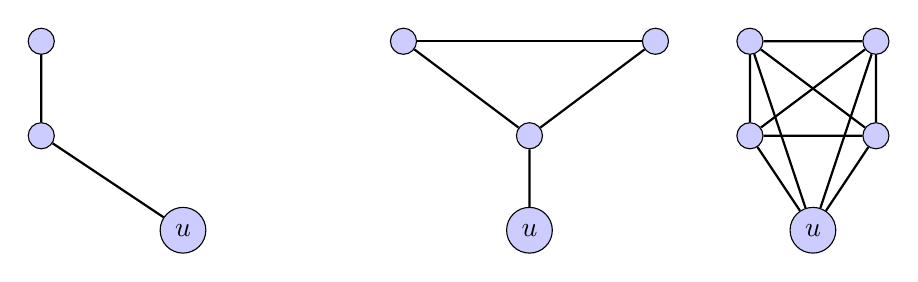
\begin{tikzpicture}
    [scale=.8,auto=left,every node/.style={circle, draw, black,
    fill=blue!20, minimum size = 2pt}]
    \node (n1) at (-1,1){$u$};
    \node (n2) at (-3.25,4)  {};
    \node (n3) at (-3.25,2.5)  {};
    \node (x1) at (4.5,1){$u$};
    \node (x2) at (2.5,4)  {};
    \node (x3) at (4.5,2.5)  {};
    \node (x4) at (6.5,4)  {};
    \node (c1) at (8,2.5){};
    \node (c2) at (8,4)  {};
    \node (c3) at (9,1)  {$u$};
    \node (c4) at (10,2.5) {};
    \node (c5) at (10,4)  {};
    \foreach \from/\to in {n1/n3,n3/n2,
    x1/x3,x2/x3,x2/x4,x3/x4,
    c1/c2,c1/c3,c1/c4,c1/c5,c2/c3,c2/c4,c2/c5,c3/c4,c3/c5,c4/c5}
    \draw[thick] (\from) -- (\to);
    \end{tikzpicture}
    \caption{From left to right, the subgraphs induced by the
    following subsets from Table~\ref{tab.margMRplus1SA}: 1-defective
    clique \{RF, SM, ECP ($u$)\}; 2-defective clique \{CAVF, Coma,
    RF, PDX-Unacc ($u$)\}; clique \{CoagHD, NV, PNA, SM, FED
    ($u$)\}. The added vertex $u$ is labeled in each graph.}
    \label{fig.defclq123}
\end{figure}

Our final experiments assess the performance of
Algorithm~\ref{alg.MargBKMMRC} when initialized with a nonempty $C^0$.
Tables~\ref{tab.margMRplus1t4} and~\ref{tab.margMRplus2t4} report
results complementary to those in Table~\ref{tab.mimicXBKdeletion}
and exhibit trends consistent with Table~\ref{tab.margMRplus1SA}.
These results identify the diseases most consequential to monitor when
a patient already carries a known set of diagnoses, which is the
primary purpose of the marginal mortality rate analysis.

\begin{table}[htbp]
\centering
\resizebox{\textwidth}{!}{%
\begin{tabular}{lclcrrr}
\toprule
{$C^0$} & \multicolumn{1}{c}{{$\mu(C^0)$}} & {Additional disease $u$}
& {$\mu(C^0 \cup \{u\})$} & {Increase} & Time & \#RC \\
\midrule
\multirow{3}{*}{SM} & 0.70 & ARF & 0.85 & 22\% &
\multirow{3}{*}{\numprint{52}} & \multirow{3}{*}{52} \\
 & 0.70 & CP & 0.83 & 20\% & & \\
 & 0.70 & PNAS & 0.83 & 19\% & & \\
\midrule
\multirow{3}{*}{RF, SM} & 0.84 & CNTN & 0.90 & 8\% &
\multirow{3}{*}{\numprint{44}} & \multirow{3}{*}{44} \\
 & 0.84 & Aphleb & 0.89 & 7\% & & \\
 & 0.84 & DKU & 0.89 & 6\% & & \\
\midrule
\multirow{1}{*}{CAVF, Coma, RF} & 0.90 & FED & 0.91 & 1\% &
\multirow{1}{*}{\numprint{2}} & \multirow{1}{*}{2} \\
\midrule
\multirow{2}{*}{CoagHD, NV, PNA, SM} & 0.94 & FED & 0.94 & 0\% &
\multirow{2}{*}{\numprint{3}} & \multirow{2}{*}{3} \\
 & 0.94 & PDX-Unacc & 0.94 & 0\% & & \\[3pt]
\bottomrule
\end{tabular}%
}
\caption{Top-3 Most Lethal Cliques Formed by the Addition of a Single
Disease}
\label{tab.margMRplus1t4}
\end{table}

\begin{table}[htbp]
\centering
\resizebox{\textwidth}{!}{%
\begin{tabular}{lclcrrr}
\toprule
{$C^0$} & \multicolumn{1}{c}{{$\mu(C^0)$}} & {Additional diseases
$u,v$} & {$\mu(C^0 \cup \{u,v\})$} & {Increase} & {Time} &
{\#RC} \\
\midrule
\multirow{3}{*}{SM} & 0.70 & SEPTL, PHD & 0.91 & 31\% &
\multirow{3}{*}{\numprint{787}} & \multirow{3}{*}{\numprint{787}} \\
 & 0.70 & ARF, Phleb & 0.90 & 29\% & & \\
 & 0.70 & ND, PHD & 0.90 & 29\% & & \\
\midrule
\multirow{3}{*}{RF, SM} & 0.84 & DKU, CNTN & 0.94 & 12\% &
\multirow{3}{*}{\numprint{748}} & \multirow{3}{*}{\numprint{748}} \\
 & 0.84 & CNTN, GSS & 0.94 & 12\% & & \\
 & 0.84 & CNTN, SEPT & 0.94 & 12\% & & \\
\midrule
\multirow{1}{*}{CAVF, Coma, RF} & 0.90 & FED & 0.91 & 1\% &
\multirow{1}{*}{\numprint{2}} & \multirow{1}{*}{2} \\
\midrule
\multirow{2}{*}{CoagHD, NV, PNA, SM} & 0.94 & FED, PDX-Unacc & 0.94
& 0\% & \multirow{2}{*}{\numprint{4}} & \multirow{2}{*}{4} \\
 & 0.94 & PDX-Unacc & 0.94 & 0\% & & \\[3pt]
\bottomrule
\end{tabular}%
}
\caption{Top-3 Most Lethal Cliques Formed by the Addition of Two
Diseases}
\label{tab.margMRplus2t4}
\end{table}

Table~\ref{tab.margMRplus1t4} shows that when $C^0 = \{\text{SM}\}$,
adding adult respiratory failure (ARF) yields the largest improvement,
raising its mortality rate from 0.70 to 0.85 (22\%), followed by cancer of
pancreas (CP) and pneumonia (PNAS) at 20\% and 19\%, respectively.
For $C^0 = \{\text{RF, SM}\}$, adding conditions due to neoplasm or
its treatment (CNTN) raises the rate from 0.84 to 0.90 (8\%), with
acute phlebitis (Aphleb) and diseases of kidney and ureters (DKU)
close behind at 7\% and 6\%, respectively. For larger cliques, gains
are marginal: both \{CAVF, Coma, RF\} and \{CoagHD, NV, PNA, SM\}
admit improvements of at most 1\% from any single addition.
Algorithm~\ref{alg.MargBKMMRC} completes all single-addition runs in at
most 52 seconds, confirming its
efficiency when initialized with a nonempty $C^0$.

Table~\ref{tab.margMRplus2t4} reports the results when two diseases
are added simultaneously. Larger gains are possible for smaller
initial cliques: adding SEPTL and PHD to \{SM\} raises the mortality
rate to 0.91 (31\%), and adding DKU and CNTN to \{RF, SM\} raises it
to 0.94 (12\%), each completing in under 790 seconds. For the larger cliques, the maximum gain from any two-disease
addition remains at or below 1\%, consistent with the pattern
observed in Table~\ref{tab.margMRplus1t4}. Together,
Tables~\ref{tab.margMRplus1t4} and~\ref{tab.margMRplus2t4}
demonstrate the utility of the framework for identifying which
additional diseases pose the greatest incremental mortality risk for
a patient already carrying a known set of diagnoses.

Chapter~\ref{sec.conclusion} concludes the dissertation by summarizing contributions, discussing limitations, and outlining directions for future research.
\begingroup
\clearpage
\let\clearpage\relax
\vspace*{-16pt}
\chapter[CONCLUSION AND FUTURE WORK]{CONCLUSION AND FUTURE WORK}\label{sec.conclusion}
\endgroup
The contributions of this dissertation are summarized below.

We introduce the maximum mortality rate clique problem, a
novel fractional combinatorial optimization problem defined on a
comorbidity graph derived from EHR data. Given a graph whose vertices
are ICD-coded disease categories and whose edges reflect statistically
significant pairwise co-occurrence measured via the Ochiai
coefficient, MMRCP seeks the $\ell$-frequent clique that maximizes
the mortality rate of the patient population simultaneously diagnosed
with all diseases in the clique. We also introduce a size-restricted
variant and the maximum marginal mortality rate clique problem, which
identifies the diseases whose addition to a known clique most elevates
the mortality rate of the combined cluster. The comorbidity graph used
throughout is constructed from MIMIC-IV using mappings from ICD codes
to disease categories via the CCS and CCSR tools, yielding a graph with
467 vertices and \numprint{8539} edges.

We establish the key theoretical properties of MMRCP. We prove that
the mortality rate function is neither additive nor monotonic, ruling
out simple greedy or local-search strategies and constituting the
fundamental structural obstacle that motivates the solution methods
developed in this dissertation. We establish the computational
hardness of MMRCP through three NP-completeness theorems.

We develop two exact combinatorial algorithms for MMRCP. The first is
a modified Bron--Kerbosch algorithm that enumerates all
$\ell$-frequent cliques while pruning branches that violate the
frequency constraint. The second is a combinatorial branch-and-bound
algorithm that incorporates an upper-bounding scheme to prune
branches whose mortality rate cannot improve upon the current
incumbent, enabling substantially faster search.

We present two MILP formulations for MMRCP. The first linearizes the
fractional mortality rate objective via auxiliary product variables,
and the second applies the Charnes--Cooper transformation. Both are
implemented with delayed constraint generation, but become
intractable as the patient population grows due to the proliferation
of patient-indexed constraints, confirming the need for alternative
strategies on large-scale instances.

To overcome these scalability limitations, we introduce a logic-based
Benders decomposition framework that eliminates all
patient-indexed variables, using only the clique incidence vector and
a scalar representing the mortality rate. Optimality cuts take the
form of simple no-good inequalities anchored at known $\ell$-frequent
cliques, and feasibility cuts are cover inequalities derived from
minimal non-$\ell$-frequent cliques. The reformulation is embedded in
a decomposition branch-and-cut algorithm with a root node relaxation
strengthened by upper-bound-based valid inequalities.

We develop a hybrid LBBD variant that integrates the combinatorial
branch-and-bound algorithm to generate stronger valid inequalities
within the decomposition framework. The combinatorial algorithm is
invoked at branch-and-cut tree nodes on a substantially smaller
induced subgraph, producing cuts that tighten the master problem far
more than the corresponding simple no-good cuts. The hybrid variant
substantially outperforms both the pure LBBD and the direct MILP
formulations across all tested instances, and is the only method to
prove optimality on the largest instances within the time limit.

We further demonstrate the flexibility of the hybrid variant to
incorporate side constraints on the cliques. As an example, we
introduce an age-based constraint that limits the proportion of
patients aged 60 or older across the diseases in the selected clique.
Incorporating this constraint reveals a qualitatively different class
of lethal cliques centered on systemic and metabolic disease
interactions---such as combinations of alcohol-related disorders, liver
disease, and acute renal failure---whose lethality is unlikely to be explained primarily by the elevated baseline mortality of elderly patients. We also introduce a cancer-containing constraint requiring at least one
cancerous diagnosis in the selected clique, yielding clinically
distinct high-mortality clusters; notably, combinations anchored at
secondary malignancies and conditions due to neoplasm treatment are
among the most lethal identified on the complete dataset. Both
constrained variants are solved to optimality across all cohort sizes
and the complete dataset. Side constraints of this form can be
seamlessly incorporated into the hybrid LBBD framework without
modifying the combinatorial branch-and-bound algorithm, underscoring
its advantage.

We apply an adaptation of the modified Bron--Kerbosch algorithm,
extended to enforce a clique-size bound and to enumerate the top-$K$
highest-mortality cliques, to the complete MIMIC-IV dataset of
\numprint{223291} patients, identifying the most lethal disease
cliques across a range of clique sizes. The algorithm scales
efficiently to this population. We further demonstrate the
framework's ability to explore the comorbidity graph broadly by
analyzing a reduced cohort after removing the two most dominant
conditions, revealing a qualitatively different set of high-mortality
comorbidity patterns. The marginal mortality rate analysis, which uses
the same algorithm initialized with a known clique, identifies
diseases whose addition to an existing diagnosis cluster most elevates
mortality risk.

Python implementations of all methods are available in the online repository~\citep{Diss-GithubRepo}.

Parts of this dissertation have appeared in the following publications,
the first published and the second currently under review.
\begin{itemize}
    \item ``Identifying Most Lethal Cliques in Disease Comorbidity
    Graphs,'' \cite{VaghfiMohebbi2025lethalclique}, \textit{IISE
    Transactions on Healthcare Systems Engineering}, 15(2), 183--200.
    Selected by the Editor-in-Chief of \textit{ISE Magazine}.
    \item ``Exact Approaches for the Maximum Mortality Rate Clique
    Problem,'' Preprint available on \hl{Optimization Online}.
\end{itemize}

\paragraph{Limitations.}
We recognize some limitations of this work. The MIMIC-IV dataset is
derived from a single academic medical center, which may limit the
generalizability of the specific disease clusters identified. We note
that while the proposed methods were initially developed and evaluated
on another EHR dataset comprising millions of patient encounters,
access to this dataset was withdrawn during the development of this
work; consequently, those results are not included in the present
study. The one-year post-discharge mortality definition used in
MIMIC-IV means that findings may differ under alternative mortality
windows or definitions, such as in-hospital mortality alone. As with
any study based on coded diagnoses, the quality of results is
sensitive to the completeness and accuracy of ICD coding practices.
External validation using diverse EHR systems and healthcare settings
would strengthen confidence in the robustness of the methods and the
results.

\paragraph{Future Directions.}
The side-constraint framework can be extended to encode other clinically
important requirements based on demographic, socioeconomic, or
treatment-related characteristics, enabling targeted investigations
of specific patient subpopulations. Applying the framework to larger,
multi-institution EHR datasets would support broader validation and
the discovery of previously understudied lethal disease combinations.

In clinical practice, rapid identification of high-mortality disease
combinations can directly inform time-sensitive decisions. A
clinician assessing a patient already carrying several diagnoses may
need to know quickly which additional co-occurring conditions elevate
mortality risk most sharply, in order to prioritize monitoring,
adjust treatment protocols, or initiate early intervention. Exact
methods, while optimal, may be too slow for interactive clinical use.
Developing fast heuristic approaches that can return high-quality
solutions within seconds would make the framework practical for
real-time decision support. Building on this, a natural direction is
the development of a decision-support tool that accepts a
clinician-specified set of diseases and identifies, via a heuristic
engine running in the background, the co-occurring diseases most
associated with elevated mortality in the underlying EHR dataset. A
web-based or locally deployable prototype of such a tool is
illustrated in Figure~\ref{fig.tool}. The development of this tool is an ongoing project by the author.
\begin{figure}[htbp]
    \centering
    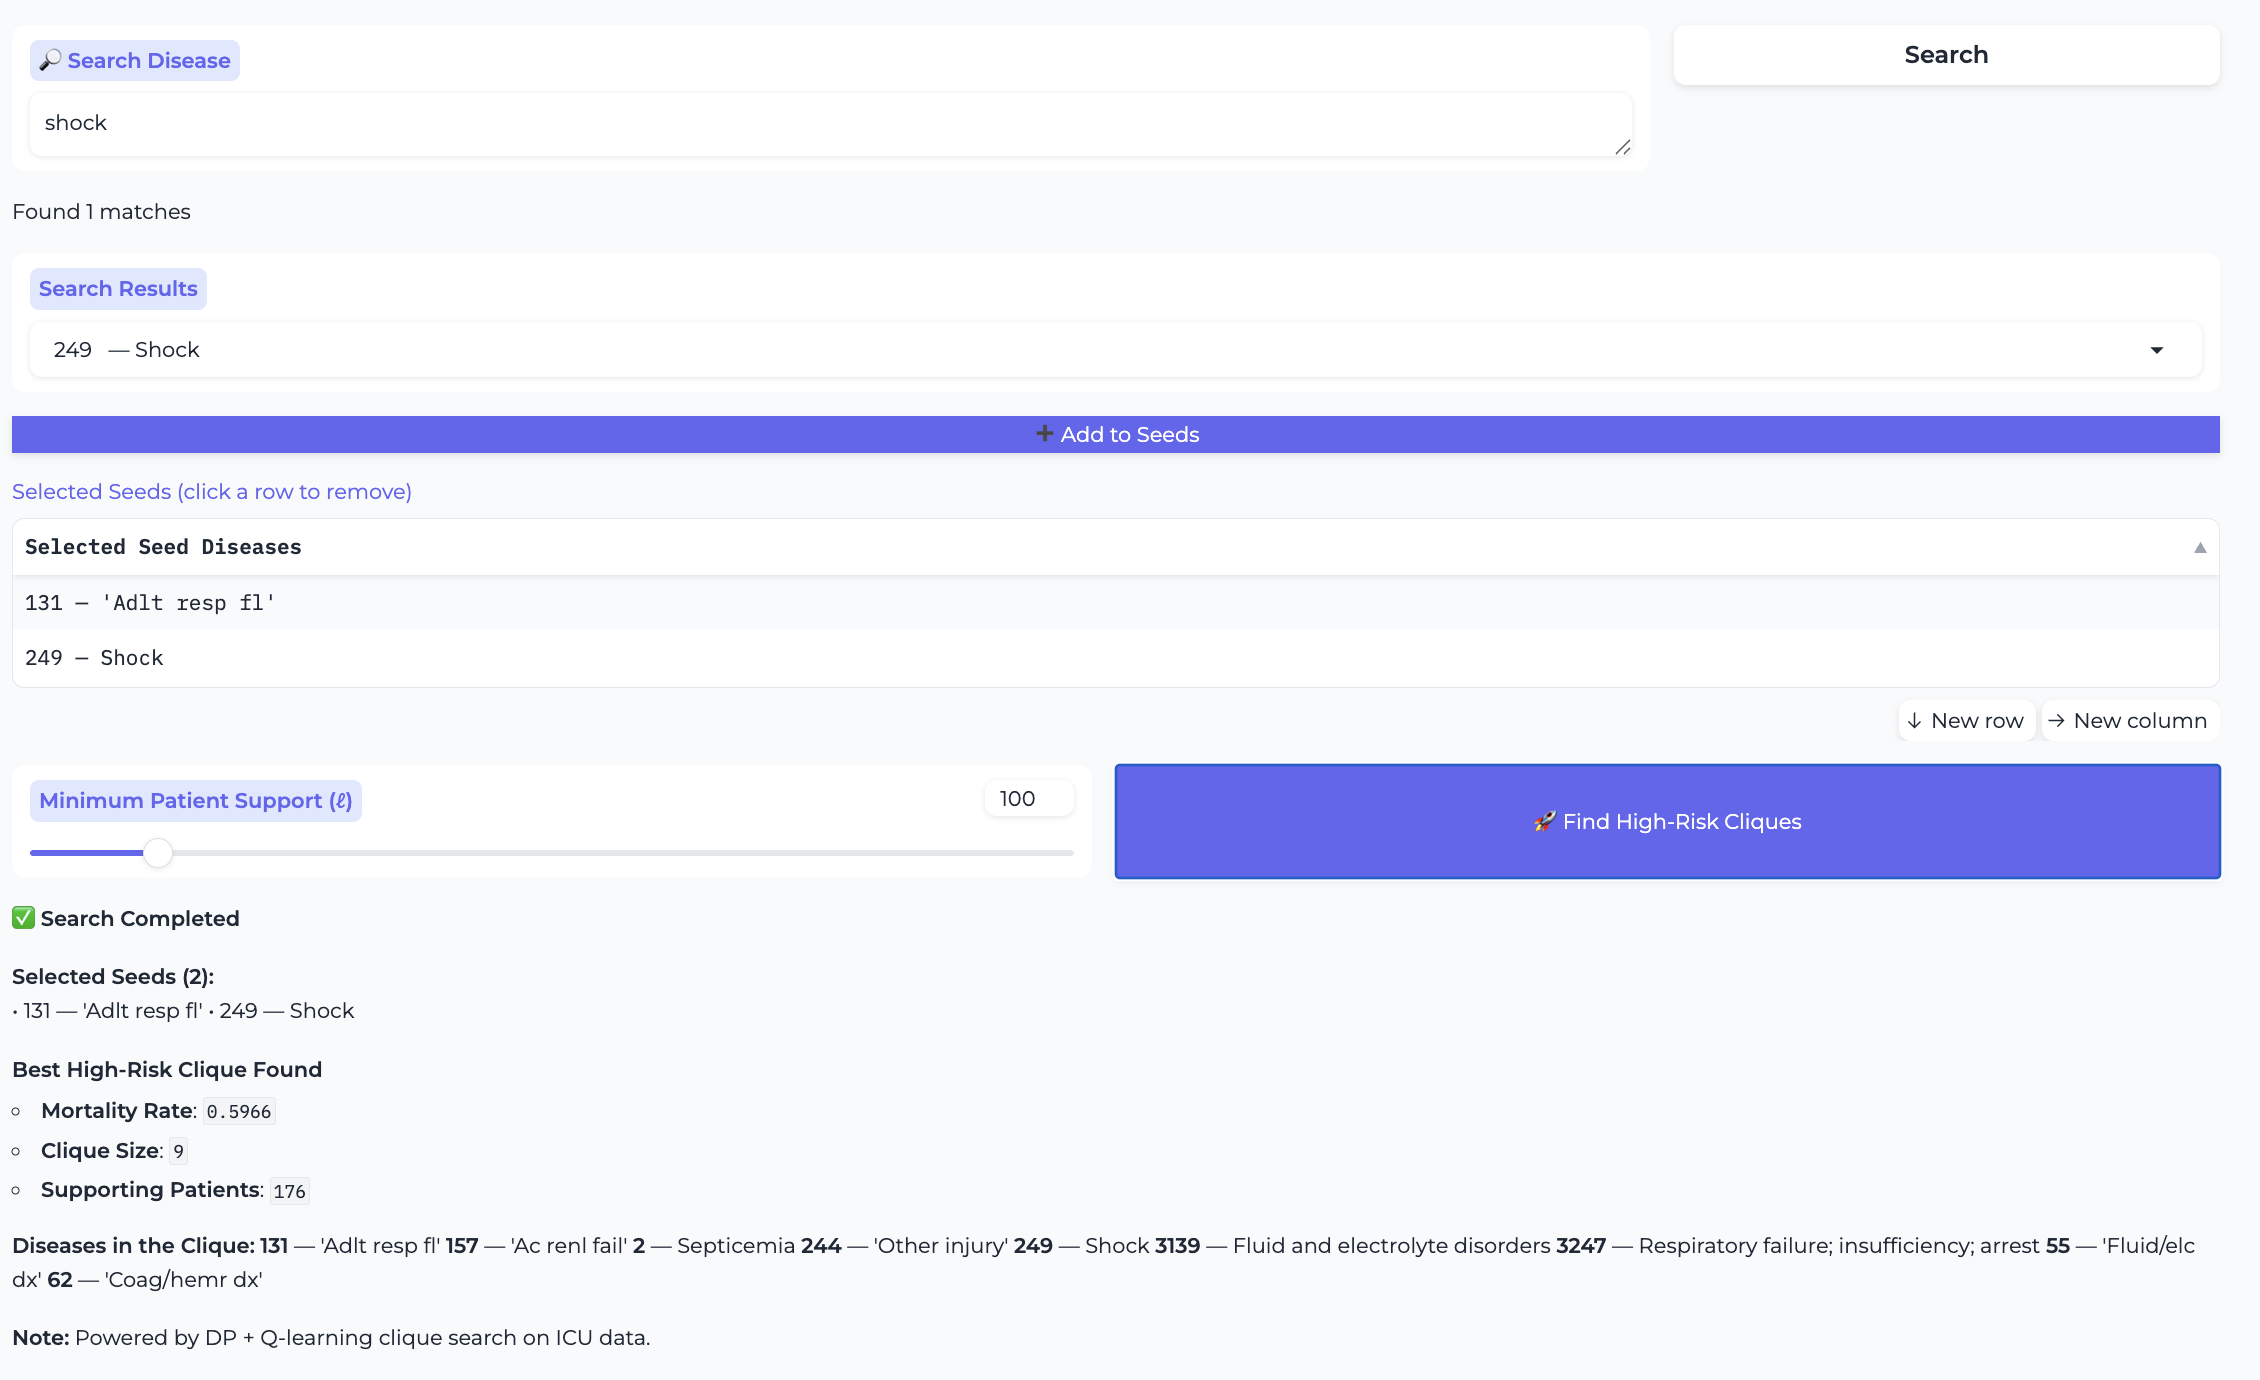
\includegraphics[width=1\textwidth]{Proto.png}
    \caption{Prototype User Interface for Identifying High-Risk
    Disease Cliques}
    \label{fig.tool}
\end{figure}
% \input{chapter1}
% \input{chapter2}
% \input{chapter3}
% \input{chapter4}
% Include as many chapters as you would like! Add other lines like the following:
%\input{anotherchapter}
%\input{conclusions}
% But don't forget to make a TeX file for each in the same folder!

%%%%%%%%%%%%%%%%%%%%%%%%%%%%%%%%%%% NOTICE %%%%%%%%%%%%%%%%%%%%%%%%%%%%%%%%%%%
% This template is set up to use BiBTeX data and automatically generate the
% bibliography based ONLY on what references you cite, so you can have a large
% bib file and only pull what you need.
%
% If, however, you want all references in your BiBTeX file to be listed in the
% references section, EVEN IF THEY WERE NOT SPECIFICALLY CITED SOMEWHERE IN
% THE DISSERTATION, then you must uncomment the following line:

%\nocite{*}

%%%%%%%%%%%%%%%%%%%%%%%%%%%%%%%%%%%%%%%%%%%%%%%%%%%%%%%%%%%%%%%%%%%%%%%%%%%%%%

%%% You can use BibTeX generated references, or type references out yourself.
%%% You can download BibTeX information from MathSciNet and 
%%% insert it into the references.bib file. 
% \usepackage{apacite}
% \bibliographystyle{apacite}
\bibliographystyle{apalike} % Other common styles: osustyle.bst, abbrv, amsalpha, ieeetr, alpha
\renewcommand\bibname{\centering REFERENCES}

% Comment out the next line if you wish to do a manual bibliography:
\begingroup
\clearpage% Manually insert \clearpage
\let\clearpage\relax% Remove \clearpage functionality
\vspace*{-16pt}% Insert needed vertical retraction
\bibliography{references.bib}
\endgroup

% Uncomment the rest of this for a manual bibliography:
% \begin{thebibliography}{bg}
% \interlinepenalty=10000
% \bibitem{K1}
% R.  Adler, The Geometry of Random Fields, Wiley, Chichester, 1981.
% 
% \bibitem{ApostolAnalyticBook}
% V. Andrievskii, Weighted polynomial inequalities in the complex plane, J. Approx. Theory, 164 (2012), 1165--1183.
% 
% \bibitem{LiCai}
% A. Granville and I. Wigman, The zeros of random trignometric polynomials, Amer. J. Math. 133 (2011), 295--357.
% 
% \bibitem{HM}
% J. Hammersley, The zeros of a random polynomial, Proc. of the Third Berk. Sym. on Math. Stat. and Prob. 1954-1955 vol. II, University of Cal. Press, Berkeley and Los Angeles (1956) 89--111.
% 
% \end{thebibliography}

%%%%%%%%%%%%%%%%%%%%%%%%%%%%%%%%%%% NOTICE %%%%%%%%%%%%%%%%%%%%%%%%%%%%%%%%%%%
% You may comment out the following line if you do not have any appendices:
% \appendix
% \include{chapter-appendix}

% \begingroup
% % \clearpage% Manually insert \clearpage
% 
% \vspace*{-16pt}% Insert needed vertical retraction
% \chapter*{\centerline{APPENDICES}}
% \endgroup

% % \begin{center}
% % {\bfseries Title of Appendix (Not Numbered)}
% % \end{center}

% \section*{Appendix A: Detailed Computational Results}\label{App.tableDeets}
% \addcontentsline{toc}{chapter}{Appendix A: Detailed Computational Results}
% \renewcommand{\thechapter}{A}
% \numberwithin{equation}{chapter}
% \setcounter{equation}{0}
% %\setcounter{theorem}{0}

\appendix

\chapter{Pseudocodes}
\label{App.Pseudos}
\numberwithin{equation}{chapter}
\setcounter{equation}{0}

% \resizebox{\linewidth}{!}{
\footnotesize{
\begin{algorithm}[H]
    \KwIn{$\langle P, \widetilde{P}, A, G=(V,E), \ell, b\rangle$ and initial clique $C^0$ (possibly empty) such that $|C^0| < b$} 
    \KwOut{Max-heap $\texttt{Q}$ of feasible cliques with mortality rate as priority}
    $\texttt{Q} \gets \emptyset$\\
    \If{$C^0\ne\emptyset$}{Insert $C^0$ in $\texttt{Q}$ with priority $\mu(C^0)$\\
    $C \gets C^0$, $L \gets \bigcap\limits_{u \in C^0}N(u)$, and $\texttt{Den} \gets \bigcap\limits_{u \in C^0} A_u$}
    \Else{$C \gets \emptyset$, $L \gets V$, and $\texttt{Den} \gets P$}
    \SetKwFunction{FBronKerbosch}{Bron-Kerbosch}
    \FBronKerbosch{$C,L,\texttt{Den}$}\\
    \KwRet{$\texttt{Q}$}\\

    \SetKwProg{Fn}{Function}{}{}
    \Fn{\FBronKerbosch{$C,L,\texttt{Den}$}}{
     \If{$|C|=b$ \text{or} $L = \emptyset$   \label{step.terminate} } {\KwRet}
        \For{$v \in L$ }{
            $\texttt{NewDen} \gets \texttt{Den} \cap A_v$\\
            \If{$|\texttt{NewDen}| \ge \ell$}{
                $\mu \gets \frac{|\widetilde{P} \cap \texttt{NewDen}|}{|\texttt{NewDen}|}$\\
                $C \gets C \cup \{v\}$\\
                \If{$C \notin \texttt{Q}$}{
                Insert $C$ in $\texttt{Q}$ with priority $\mu$\\
                }
                \FBronKerbosch{$C, L\cap N(v),  \texttt{NewDen}$}\\
            }
            $L \gets L \setminus \{v\}$\\
        }
        \KwRet %$Q$
    }
\caption{Enumerating Highest (Marginal) Mortality Rate Cliques}
\label{alg.MargBKMMRC}
\end{algorithm}}

\chapter{Detailed Computational Results}
\label{App.tableDeets}

\numberwithin{equation}{chapter}
\setcounter{equation}{0}

The appendix tables summarize the numerical results using the following column headings. The column ``Size'' represents the patient cohort size, while ``No.'' denotes the sample identifier. ``Best Obj'' gives the best objective value obtained, and ``Time'' reports the wall-clock computation time, rounded down to the nearest second; ``TO'' indicates that the algorithm terminated upon reaching the 2-hour time limit. The column ``Gap'' shows the percentage optimality gap at termination, where a value of zero signifies that an optimal solution was found within the solver tolerance. The number of explored branch-and-cut nodes is reported in ``\#BC Nodes'', and ``\#RC'' gives the number of recursive calls. The column ``\#CBB Calls'' records the number of invocations of the CBB algorithm, while ``\#CBB Rec'' reports the total number of recursive calls within CBB. In addition, ``\#Opt Cuts'' and ``\#Feas Cuts'' indicate the numbers of optimality and feasibility cuts generated, respectively, whereas ``\#CBB Cuts'' reports the number of CBB cuts produced by the hybrid LBBD algorithm. The ``Clique'' column identifies the diseases comprising the maximum clique for each sample. Finally, ``Avg'' reports the average over the five samples, and ``Range'' provides the corresponding minimum and maximum observed values. Disease names are abbreviated for brevity and space limitations; the complete disease names are listed in Appendix~\ref{App.Abbs}.

A dash ``-'' indicates that no value was reported by the solver for that metric. An asterisk ``$^{*}$" in Tables~\ref{tab.Gam} and~\ref{tab.Extension} indicates that although a gap is reported by the solver, the obtained solution matches the result from the Bron--Kerbosch and CBB algorithms.


\begin{table}[htbp]
\centering
\scriptsize{\begin{tabular}{lllrrrrr}
 \toprule
Size & No. & Clique & Best Obj & \multicolumn{2}{c}{BK} & \multicolumn{2}{c}{CBB} \\
 &  &  &  & Time & \#RC & Time & \#RC \\
\midrule
\multirow{5}{*}{\numprint{1000}}
 & 1 & PDX-Unacc, AURF & 0.45 & $<1$ & \numprint{40} & $<1$ & \numprint{14} \\
 & 2 & ARF & 0.49 & $<1$ & \numprint{48} & $<1$ & \numprint{15} \\
 & 3 & RCU, OA & 0.46 & $<1$ & \numprint{44} & $<1$ & \numprint{15} \\
 & 4 & FED, PDX-Unacc & 0.41 & $<1$ & \numprint{43} & $<1$ & \numprint{20} \\
 & 5 & FD & 0.43 & $<1$ & \numprint{40} & $<1$ & \numprint{10} \\
\midrule
\multirow{5}{*}{\numprint{5000}}
 & 1 & MALN, PDX-Unacc, OACE & 0.87 & 1 & \numprint{4580} & $<1$ & \numprint{689} \\
 & 2 & OACE, AURF, FED & 0.88 & 1 & \numprint{3893} & $<1$ & \numprint{547} \\
 & 3 & CHF-NH, ARF, CKD & 0.72 & 1 & \numprint{3136} & $<1$ & \numprint{454} \\
 & 4 & SM & 0.77 & 1 & \numprint{2623} & $<1$ & \numprint{418} \\
  & 5 & FD, CHF-NH, CardArr & 0.74 & 1 & \numprint{2542} & $<1$ & \numprint{492} \\
\midrule
\multirow{5}{*}{\numprint{10000}}
 & 1 & PDX-Unacc, PNA, FED, OACE & 0.92 & 3 & \numprint{31562} & 1 & \numprint{6052} \\
 & 2 & PDX-Unacc, DLM, CD, OACE & 0.92 & 3 & \numprint{31545} & 1 & \numprint{5324} \\
 & 3 & SM, RCU, ONSD & 0.83 & 2 & \numprint{23101} & 1 & \numprint{4954} \\
 & 4 & OA, SM & 0.83 & 2 & \numprint{21784} & 1 & \numprint{4730} \\
 & 5 & SM, RCU, DOA & 0.81 & 2 & \numprint{20643} & 1 & \numprint{3640} \\
\midrule
\multirow{5}{*}{\numprint{15000}}
 & 1 & OACE, SHK & 0.95 & 9 & \numprint{122916} & 4 & \numprint{21387} \\
 & 2 & SEPT, OSNSD, PDX-Unacc, RF, OACE & 0.94 & 9 & \numprint{126861} & 4 & \numprint{21775} \\
 & 3 & OSNSD, AURF, PDX-Unacc, RF, OACE & 1.00 & 7 & \numprint{97075} & 3 & \numprint{13593} \\
 & 4 & SEPT, CD, PDX-Unacc, FED, OACE & 0.96 & 8 & \numprint{117050} & 4 & \numprint{19757} \\
 & 5 & DOA, ONSD, SM & 0.89 & 5 & \numprint{71752} & 2 & \numprint{13183} \\
\midrule
\multirow{5}{*}{\numprint{20000}}
 & 1 & OACE, SHK, RF & 0.97 & 27 & \numprint{332591} & 8 & \numprint{61953} \\
 & 2 & OACE, AURF, COPD-BE, PDX-Unacc, FED & 0.96 & 26 & \numprint{312853} & 8 & \numprint{57524} \\
 & 3 & OACE, RF, PNA, AURF, PDX-Unacc & 0.99 & 23 & \numprint{271897} & 7 & \numprint{47423} \\
 & 4 & OACE, AURF, SHK, PDX-Unacc, FED & 0.96 & 25 & \numprint{301779} & 8 & \numprint{58434} \\
 & 5 & OACE, DLM, RF, PDX-Unacc, CoagHD & 0.97 & 22 & \numprint{259805} & 7 & \numprint{43931} \\
\midrule
\multirow{5}{*}{\numprint{25000}}
 & 1 & OACE, RF, PNA, OSNSD, PDX-Unacc & 0.97 & 53 & \numprint{702379} & 26 & \numprint{150611} \\
 & 2 & CA, OACE, DLM, RF, HF, PDX-Unacc & 0.97 & 47 & \numprint{615018} & 23 & \numprint{134531} \\
 & 3 & NCD, OACE, AURF, PDX-Unacc, OSNSD & 0.98 & 42 & \numprint{541644} & 20 & \numprint{112198} \\
 & 4 & OACE, HF, PDX-Unacc, SHK, FED & 0.97 & 46 & \numprint{595396} & 23 & \numprint{132610} \\
 & 5 & SEPT, OACE, DLM, PDX-Unacc, CoagHD & 0.98 & 45 & \numprint{576175} & 20 & \numprint{107244} \\
\midrule
\multirow{5}{*}{\numprint{30000}}
 & 1 & HCSH, ARF, ONSD, RCU & 0.83 & 83 & \numprint{1387200} & 2 & \numprint{14725} \\
 & 2 & CHF-NH, DOA, CUS & 0.88 & 78 & \numprint{1280684} & 2 & \numprint{11290} \\
 & 3 & DOA, CardArr, GD, RCU, CA & 0.87 & 66 & \numprint{1032733} & 2 & \numprint{12693} \\
 & 4 & CardArr, HCSH, CHF-NH, CUS & 0.84 & 67 & \numprint{1064147} & 2 & \numprint{11518} \\
 & 5 & HCSH, SHK, OA & 0.85 & 70 & \numprint{1061875} & 2 & \numprint{10960} \\
\midrule
\multirow{1}{*}{\numprint{223291}}
 &  & - & - & TO & - & TO & - \\
 \bottomrule
\end{tabular}}
\caption{Comparing the Modified Bron--Kerbosch Algorithm and CBB Algorithm}
\label{tab.BKCBB}
\end{table}

\begin{table}[htbp]
\centering
\scriptsize 
  \begin{tabular}{l l| r r r | r r r | r r r}
    \toprule
    Size & No. & \multicolumn{3}{c|}{Formulation~\eqref{form.milp} - Aggregation} & \multicolumn{3}{c|}{Formulation~\eqref{form.milp} - No Aggregation} & \multicolumn{3}{c}{Formulation~\eqref{form.CCIP}} \\ \midrule
     & & Gap & Time & \#BC Nodes & Gap & Time & \#BC Nodes & Gap & Time & \#BC Nodes \\
    \midrule
    \multirow{5}{*}{\numprint{1000}}
     & \numprint{1} & \numprint{0} & \numprint{17} & \numprint{1} & \numprint{0} & \numprint{71} & \numprint{3} & \numprint{0} & \numprint{2} & \numprint{215} \\
     & \numprint{2} & \numprint{0} & \numprint{16} & \numprint{349} & \numprint{0} & \numprint{73} & \numprint{1} & \numprint{0} & \numprint{3} & \numprint{242} \\
     & \numprint{3} & \numprint{0} & \numprint{34} & \numprint{505} & \numprint{0} & \numprint{68} & \numprint{1} & \numprint{0} & \numprint{4} & \numprint{415} \\
     & \numprint{4} & \numprint{0} & \numprint{21} & \numprint{517} & \numprint{0} & \numprint{75} & \numprint{1} & \numprint{0} & \numprint{3} & \numprint{176} \\
     & \numprint{5} & \numprint{0} & \numprint{35} & \numprint{1} & \numprint{0} & \numprint{66} & \numprint{1} & \numprint{0} & \numprint{4} & \numprint{198} \\
    \midrule
    \multirow{5}{*}{\numprint{5000}}
     & \numprint{1} & \numprint{14} & TO & \numprint{1535817} & \numprint{14} & TO & \numprint{6256} & \numprint{0} & \numprint{1033} & \numprint{10118} \\
     & \numprint{2} & \numprint{13} & TO & \numprint{764563} & \numprint{13} & TO & \numprint{6550} & \numprint{0} & \numprint{1450} & \numprint{11551} \\
     & \numprint{3} & \numprint{54} & TO & \numprint{708721} & \numprint{38} & TO & \numprint{5941} & \numprint{0} & \numprint{863} & \numprint{5624} \\
     & \numprint{4} & \numprint{36} & TO & \numprint{2916160} & \numprint{45} & TO & \numprint{9894} & \numprint{0} & \numprint{850} & \numprint{10519} \\
     & \numprint{5} & \numprint{41} & TO & \numprint{1075728} & \numprint{47} & TO & \numprint{5440} & \numprint{0} & \numprint{3770} & \numprint{9505} \\
    \midrule
    \multirow{5}{*}{\numprint{10000}}
     & \numprint{1} & \numprint{8} & TO & \numprint{8492} & - & TO & \numprint{0} & \numprint{8} & TO & \numprint{7191} \\
     & \numprint{2} & \numprint{9} & TO & \numprint{4861} & \numprint{622} & TO & \numprint{1} & \numprint{8} & TO & \numprint{6054} \\
     & \numprint{3} & \numprint{38} & TO & \numprint{4307} & \numprint{95} & TO & \numprint{1} & \numprint{24} & TO & \numprint{9682} \\
     & \numprint{4} & \numprint{20} & TO & \numprint{4735} & \numprint{84} & TO & \numprint{1} & \numprint{20} & TO & \numprint{29100} \\
     & \numprint{5} & \numprint{67} & TO & \numprint{7195} & \numprint{103} & TO & \numprint{1} & \numprint{0} & \numprint{6986} & \numprint{24184} \\
    \midrule
    \multirow{5}{*}{\numprint{15000}}
     & \numprint{1} & \numprint{57} & TO & \numprint{7076} & - & TO & \numprint{0} & \numprint{5} & TO & \numprint{5906} \\
     & \numprint{2} & \numprint{23} & TO & \numprint{5266} & - & TO & \numprint{0} & \numprint{19} & TO & \numprint{5530} \\
     & \numprint{3} & \numprint{6} & TO & \numprint{5867} & \numprint{381} & TO & \numprint{1} & \numprint{0} & \numprint{3554} & \numprint{2342} \\
     & \numprint{4} & \numprint{32} & TO & \numprint{6516} & \numprint{162} & TO & \numprint{1} & \numprint{4} & TO & \numprint{5171} \\
     & \numprint{5} & \numprint{50} & TO & \numprint{6431} & \numprint{576} & TO & \numprint{1} & \numprint{28} & TO & \numprint{5795} \\
    \midrule
    \multirow{5}{*}{\numprint{20000}}
     & \numprint{1} & \numprint{23} & TO & \numprint{4469} & - & TO & \numprint{0} & \numprint{31} & TO & \numprint{3041} \\
     & \numprint{2} & \numprint{51} & TO & \numprint{5943} & - & TO & \numprint{0} & \numprint{20} & TO & \numprint{3913} \\
     & \numprint{3} & \numprint{11} & TO & \numprint{4004} & - & TO & \numprint{0} & \numprint{14} & TO & \numprint{3621} \\
     & \numprint{4} & \numprint{4} & TO & \numprint{5054} & - & TO & \numprint{0} & \numprint{7} & TO & \numprint{2868} \\
     & \numprint{5} & \numprint{33} & TO & \numprint{6733} & \numprint{417} & TO & \numprint{1} & \numprint{71} & TO & \numprint{1403} \\
    \midrule
    \multirow{5}{*}{\numprint{25000}}
     & \numprint{1} & \numprint{24} & TO & \numprint{7350} & - & TO & \numprint{0} & \numprint{81} & TO & \numprint{2758} \\
     & \numprint{2} & \numprint{88} & TO & \numprint{50} & - & TO & \numprint{0} & \numprint{7} & TO & \numprint{1319} \\
     & \numprint{3} & \numprint{25} & TO & \numprint{40} & - & TO & \numprint{0} & \numprint{186} & TO & \numprint{877} \\
     & \numprint{4} & \numprint{9} & TO & \numprint{5643} & - & TO & \numprint{0} & \numprint{145} & TO & \numprint{1712} \\
     & \numprint{5} & \numprint{5} & TO & \numprint{6411} & - & TO & \numprint{0} & \numprint{70} & TO & \numprint{1824} \\
    \midrule
    \multirow{5}{*}{\numprint{30000}}
     & \numprint{1} & \numprint{51} & TO & \numprint{5358} & - & TO & \numprint{0} & \numprint{87} & TO & \numprint{1908} \\
     & \numprint{2} & \numprint{38} & TO & \numprint{218} & - & TO & \numprint{0} & \numprint{254} & TO & \numprint{1360} \\
     & \numprint{3} & \numprint{476} & TO & \numprint{25} & - & TO & \numprint{0} & \numprint{154} & TO & \numprint{2040} \\
     & \numprint{4} & \numprint{50} & TO & \numprint{4284} & - & TO & \numprint{0} & \numprint{37} & TO & \numprint{1564} \\
     & \numprint{5} & \numprint{23} & TO & \numprint{1002} & - & TO & \numprint{0} & \numprint{32} & TO & \numprint{655} \\
    \midrule
    \numprint{223291} &  & - & TO & \numprint{0} & - & TO & \numprint{0} & - & TO & \numprint{0} \\
    \bottomrule
  \end{tabular}
  \caption{Comparing Direct Solution of MILP Formulations}
\label{tab.MILPs}
\end{table}

\begin{table}[htbp]
\centering
\scriptsize
\begin{tabular}{llrrrr}
\toprule
Size & No. & \multicolumn{4}{c}{Algorithm~\ref{alg.LBBDgamma}} \\ 
\midrule
 & & Gap & Time & \#Opt Cuts & \#Feas Cuts \\
\multirow{5}{*}{\numprint{1000}}
 & 1 & 0 & $<1$ & \numprint{14} & \numprint{23} \\
 & 2 & 0 & $<1$ & \numprint{17} & \numprint{50} \\
 & 3 & 0 & $<1$ & \numprint{4} & \numprint{79} \\
 & 4 & 0 & $<1$ & \numprint{21} & \numprint{92} \\
 & 5 & 0 & $<1$ & \numprint{12} & \numprint{18} \\
\midrule
\multirow{5}{*}{\numprint{5000}}
 & 1 & 0 & 4 & \numprint{1365} & \numprint{577} \\
 & 2 & 0 & 3 & \numprint{963} & \numprint{639} \\
 & 3 & 0 & 2 & \numprint{1060} & \numprint{909} \\
 & 4 & 0 & 3 & \numprint{1085} & \numprint{1039} \\
 & 5 & 0 & 2 & \numprint{783} & \numprint{728} \\
\midrule
\multirow{5}{*}{\numprint{10000}}
 & 1 & 0 & 378 & \numprint{19593} & \numprint{15620} \\
 & 2 & 0 & 347 & \numprint{19204} & \numprint{16057} \\
 & 3 & 0 & 264 & \numprint{14427} & \numprint{14480} \\
 & 4 & 0 & 240 & \numprint{13515} & \numprint{12863} \\
 & 5 & 0 & 252 & \numprint{11427} & \numprint{12036} \\
\midrule
\multirow{5}{*}{\numprint{15000}}
 & 1 & $^{*}$5 & TO & \numprint{77900} & \numprint{67228} \\
 & 2 & $^{*}$6 & TO & \numprint{79463} & \numprint{70431} \\
 & 3 & 0 & 47 & \numprint{5010} & \numprint{4452} \\
 & 4 & $^{*}$4 & TO & \numprint{92190} & \numprint{74083} \\
 & 5 & 0 & \numprint{2278} & \numprint{48852} & \numprint{47180} \\
\midrule
\multirow{5}{*}{\numprint{20000}}
 & 1 & 4 & TO & \numprint{62069} & \numprint{69195} \\
 & 2 & $^{*}$4 & TO & \numprint{64757} & \numprint{82328} \\
 & 3 & $^{*}$1 & TO & \numprint{70642} & \numprint{75180} \\
 & 4 & $^{*}$4 & TO & \numprint{77643} & \numprint{74588} \\
 & 5 & $^{*}$3& TO & \numprint{85761} & \numprint{62164} \\
\midrule
\multirow{5}{*}{\numprint{25000}}
 & 1 & 4 & TO & \numprint{64476} & \numprint{69818} \\
 & 2 & 4 & TO & \numprint{49369} & \numprint{89502} \\
 & 3 & 3 & TO & \numprint{60025} & \numprint{85746} \\
 & 4 & 4 & TO & \numprint{82039} & \numprint{59438} \\
 & 5 & $^{*}$2 & TO & \numprint{70246} & \numprint{76229} \\
\midrule
\multirow{5}{*}{\numprint{30000}}
 & 1 & 5 & TO & \numprint{58035} & \numprint{114797} \\
 & 2 & 3 & TO & \numprint{56441} & \numprint{143617} \\
 & 3 & 4 & TO & \numprint{60027} & \numprint{150718} \\
 & 4 & 3 & TO & \numprint{56445} & \numprint{140945} \\
 & 5 & 4 & TO & \numprint{75841} & \numprint{136768} \\
\midrule
\numprint{223291} &  & 3 & TO & \numprint{58825} & \numprint{42595} \\
\bottomrule
\end{tabular}
\caption{Results of Pure LBBD Algorithm for Different Instance Sizes}
\label{tab.Gam}
\end{table}

\begin{table}[htbp]
\scriptsize \centering
\centering
\begin{tabular}{llrrrrrrrr}
\toprule
Size & No. & \multicolumn{7}{c}{Algorithm~\ref{alg.hybridLBBD}} \\ \midrule
 & & Gap & Time & \#Opt Cuts & \#Feas Cuts & \#CBB Cuts & \#CBB Calls & \#CBB Rec & \#BC Nodes \\
\midrule
\multirow{5}{*}{\numprint{1000}}
 & 1 & \numprint{0} & \numprint{0} & \numprint{8} & \numprint{0} & \numprint{0} & \numprint{0} & \numprint{0} & \numprint{318} \\
 & 2 & \numprint{0} & \numprint{0} & \numprint{7} & \numprint{0} & \numprint{0} & \numprint{0} & \numprint{0} & \numprint{378} \\
 & 3 & \numprint{0} & \numprint{0} & \numprint{9} & \numprint{0} & \numprint{0} & \numprint{0} & \numprint{0} & \numprint{430} \\
 & 4 & \numprint{0} & \numprint{0} & \numprint{14} & \numprint{0} & \numprint{0} & \numprint{0} & \numprint{0} & \numprint{469} \\
 & 5 & \numprint{0} & \numprint{0} & \numprint{5} & \numprint{0} & \numprint{0} & \numprint{0} & \numprint{0} & \numprint{381} \\
\midrule
\multirow{5}{*}{\numprint{5000}}
 & 1 & \numprint{0} & \numprint{2} & \numprint{1249} & \numprint{507} & \numprint{183} & \numprint{527} & \numprint{1040} & \numprint{11062} \\
 & 2 & \numprint{0} & \numprint{2} & \numprint{904} & \numprint{542} & \numprint{70} & \numprint{312} & \numprint{495} & \numprint{8738} \\
 & 3 & \numprint{0} & \numprint{1} & \numprint{907} & \numprint{645} & \numprint{43} & \numprint{264} & \numprint{335} & \numprint{9838} \\
 & 4 & \numprint{0} & \numprint{1} & \numprint{766} & \numprint{594} & \numprint{4} & \numprint{195} & \numprint{204} & \numprint{8208} \\
 & 5 & \numprint{0} & \numprint{1} & \numprint{736} & \numprint{540} & \numprint{15} & \numprint{156} & \numprint{175} & \numprint{7954} \\
\midrule
\multirow{5}{*}{\numprint{10000}}
 & 1 & \numprint{0} & \numprint{68} & \numprint{8639} & \numprint{4764} & \numprint{6647} & \numprint{2682} & \numprint{11947} & \numprint{68543} \\
 & 2 & \numprint{0} & \numprint{64} & \numprint{7762} & \numprint{4781} & \numprint{6842} & \numprint{2242} & \numprint{7579} & \numprint{67416} \\
 & 3 & \numprint{0} & \numprint{146} & \numprint{10571} & \numprint{9619} & \numprint{3565} & \numprint{6213} & \numprint{24506} & \numprint{116124} \\
 & 4 & \numprint{0} & \numprint{125} & \numprint{9868} & \numprint{8504} & \numprint{3413} & \numprint{5884} & \numprint{23928} & \numprint{108353} \\
 & 5 & \numprint{0} & \numprint{97} & \numprint{8426} & \numprint{7641} & \numprint{2527} & \numprint{4685} & \numprint{16455} & \numprint{98459} \\
\midrule
\multirow{5}{*}{\numprint{15000}}
 & 1 & \numprint{0} & \numprint{1782} & \numprint{37201} & \numprint{6523} & \numprint{30033} & \numprint{13640} & \numprint{104373} & \numprint{247888} \\
 & 2 & \numprint{0} & \numprint{2394} & \numprint{39564} & \numprint{7257} & \numprint{34797} & \numprint{14348} & \numprint{93408} & \numprint{283938} \\
 & 3 & \numprint{0} & \numprint{7} & \numprint{577} & \numprint{45} & \numprint{189} & \numprint{61} & \numprint{384} & \numprint{3992} \\
 & 4 & \numprint{0} & \numprint{1819} & \numprint{38479} & \numprint{3742} & \numprint{28496} & \numprint{14400} & \numprint{99106} & \numprint{239752} \\
 & 5 & \numprint{0} & \numprint{412} & \numprint{15025} & \numprint{3024} & \numprint{15139} & \numprint{4967} & \numprint{24285} & \numprint{120737} \\
\midrule
\multirow{5}{*}{\numprint{20000}}
 & 1 & $^{*}$\numprint{2} & TO & \numprint{80171} & \numprint{70127} & \numprint{43431} & \numprint{59660} & \numprint{1020734} & \numprint{1755111} \\
 & 2 & $^{*}$\numprint{3} & TO & \numprint{79764} & \numprint{73172} & \numprint{42410} & \numprint{58426} & \numprint{979089} & \numprint{1729008} \\
 & 3 & \numprint{0} & TO & \numprint{80987} & \numprint{70965} & \numprint{44561} & \numprint{60810} & \numprint{913875} & \numprint{1898770} \\
 & 4 & $^{*}$\numprint{4} & TO & \numprint{89610} & \numprint{76794} & \numprint{48648} & \numprint{67473} & \numprint{1123465} & \numprint{1728209} \\
 & 5 & $^{*}$\numprint{2} & TO & \numprint{79347} & \numprint{70623} & \numprint{41677} & \numprint{58268} & \numprint{880261} & \numprint{2011960} \\
\midrule
\multirow{5}{*}{\numprint{25000}}
 & 1 & $^{*}$\numprint{3} & TO & \numprint{75160} & \numprint{73049} & \numprint{44231} & \numprint{58623} & \numprint{1677040} & \numprint{1150467} \\
 & 2 & $^{*}$\numprint{3} & TO & \numprint{82335} & \numprint{86002} & \numprint{48200} & \numprint{65717} & \numprint{1360912} & \numprint{1331444} \\
 & 3 & $^{*}$\numprint{2} & TO & \numprint{62595} & \numprint{66641} & \numprint{37470} & \numprint{49364} & \numprint{1185607} & \numprint{1575102} \\
 & 4 & \numprint{3} & TO & \numprint{79725} & \numprint{79898} & \numprint{45936} & \numprint{62952} & \numprint{1294992} & \numprint{1228444} \\
 & 5 & $^{*}$\numprint{1} & TO & \numprint{75146} & \numprint{78327} & \numprint{43072} & \numprint{58636} & \numprint{1310267} & \numprint{1365038} \\
\midrule
\multirow{5}{*}{\numprint{30000}}
 & 1 & 0 & \numprint{752} & \numprint{22737} & \numprint{26965} & \numprint{8336} & \numprint{14763} & \numprint{73165} & \numprint{513167} \\
 & 2 & 0 & \numprint{532} & \numprint{18620} & \numprint{23116} & \numprint{6683} & \numprint{11490} & \numprint{46786} & \numprint{355877} \\
 & 3 & 0 & \numprint{1102} & \numprint{20267} & \numprint{26087} & \numprint{7354} & \numprint{12553} & \numprint{52734} & \numprint{646808} \\
 & 4 & 0 & \numprint{637} & \numprint{19465} & \numprint{23505} & \numprint{6939} & \numprint{12159} & \numprint{53177} & \numprint{379999} \\
 & 5 & 0 & \numprint{559} & \numprint{18635} & \numprint{24172} & \numprint{6476} & \numprint{11347} & \numprint{47728} & \numprint{303805} \\
\midrule
\numprint{223291} &  & 2 & TO & \numprint{423} & \numprint{1} & \numprint{201} & \numprint{201} & \numprint{103857204} & \numprint{5678} \\
\bottomrule
\end{tabular}
\caption{Results of Hybrid LBBD Algorithm for Different Instance Sizes}
\label{tab.HybridLBBD}
\end{table}


% \begin{landscape}
\begin{table}[htbp]
\centering
\resizebox{\linewidth}{!}{
\begin{tabular}{lllrrrrrrrrr}
\toprule
Size & No. & Clique & Best Obj & Gap & Time & \#Opt Cuts & \#Feas Cuts & \#CBB Cuts & \#CBB Calls & \#CBB Rec & \#BC Nodes \\
\midrule
\multirow{5}{*}{\numprint{1000}}
 & 1 & SHMSA & 0.27 & 0 & $<1$ & \numprint{6} & 0 & 0 & 0 & 0 & \numprint{461} \\
 & 2 & NEMD & 0.35 & 0 & $<1$ & \numprint{7} & 0 & 0 & 0 & 0 & \numprint{402} \\
 & 3 & GD & 0.34 & 0 & $<1$ & \numprint{7} & 0 & 0 & 0 & 0 & \numprint{429} \\
 & 4 & NEMD & 0.35 & 0 & 0 & \numprint{5} & 0 & 0 & 0 & 0 & \numprint{431} \\
 & 5 & AFRD, PDX-Unacc & 0.20 & 0 & $<1$ & \numprint{3} & 0 & 0 & 0 & 0 & \numprint{510} \\
\midrule
\multirow{5}{*}{\numprint{5000}}
 & 1 & SHMSA, OLD & 0.47 & 0 & 1 & \numprint{76} & \numprint{55} & 0 & \numprint{2} & \numprint{2} & \numprint{1784} \\
 & 2 & SHMSA, RCU, E-PO & 0.45 & 0 & 1 & \numprint{78} & \numprint{56} & 0 & \numprint{3} & \numprint{3} & \numprint{1926} \\
 & 3 & GD, RCU, MD & 0.46 & 0 & 1 & \numprint{50} & \numprint{27} & 0 & 0 & 0 & \numprint{1422} \\
 & 4 & GD, DOA, MD & 0.52 & 0 & 0 & \numprint{35} & \numprint{22} & 0 & 0 & 0 & \numprint{1340} \\
 & 5 & SHMSA, OLD & 0.46 & 0 & 1 & \numprint{38} & \numprint{14} & 0 & 0 & 0 & \numprint{1419} \\
\midrule
\multirow{5}{*}{\numprint{10000}}
 & 1 & OSULD, HepF, PDX-Unacc, FED & 0.58 & 0 & 9 & \numprint{273} & \numprint{197} & \numprint{13} & \numprint{48} & \numprint{73} & \numprint{4484} \\
 & 2 & OSULD, HepF & 0.61 & 0 & 7 & \numprint{224} & \numprint{142} & \numprint{8} & \numprint{32} & \numprint{49} & \numprint{3651} \\
 & 3 & OLD, ONSD, NEMD & 0.56 & 0 & 5 & \numprint{246} & \numprint{277} & \numprint{3} & \numprint{31} & \numprint{35} & \numprint{4454} \\
 & 4 & E-AMD, MD, NEMD & 0.54 & 0 & 4 & \numprint{249} & \numprint{238} & \numprint{8} & \numprint{45} & \numprint{54} & \numprint{4428} \\
 & 5 & AD, DOA, RCU, MD & 0.47 & 0 & 3 & \numprint{152} & \numprint{94} & \numprint{5} & \numprint{15} & \numprint{24} & \numprint{2682} \\
\midrule
\multirow{5}{*}{\numprint{15000}}
 & 1 & PDX-Unacc, HepF & 0.57 & 0 & 41 & \numprint{646} & \numprint{576} & \numprint{88} & \numprint{192} & \numprint{452} & \numprint{10989} \\
 & 2 & E-AMD, MD, NORCP & 0.63 & 0 & 41 & \numprint{742} & \numprint{769} & \numprint{100} & \numprint{200} & \numprint{479} & \numprint{13416} \\
 & 3 & AFRD, PDX-Unacc, CNTN & 0.62 & 0 & 41 & \numprint{742} & \numprint{692} & \numprint{114} & \numprint{211} & \numprint{502} & \numprint{12440} \\
 & 4 & Hepatitis, OLD, FD & 0.67 & 0 & 45 & \numprint{651} & \numprint{622} & \numprint{78} & \numprint{159} & \numprint{332} & \numprint{11402} \\
 & 5 & DCP, AlcD, FD & 0.59 & 0 & 12 & \numprint{359} & \numprint{320} & \numprint{27} & \numprint{66} & \numprint{131} & \numprint{6142} \\
\midrule
\multirow{5}{*}{\numprint{20000}}
 & 1 & Hepatitis, OLD, ARenF & 0.64 & 0 & 99 & \numprint{1307} & \numprint{1306} & \numprint{249} & \numprint{464} & \numprint{1597} & \numprint{22147} \\
 & 2 & DSD, OLD & 0.63 & 0 & 131 & \numprint{1788} & \numprint{1921} & \numprint{346} & \numprint{687} & \numprint{2415} & \numprint{31567} \\
 & 3 & PDX-Unacc, NV, CNTN & 0.67 & 0 & 89 & \numprint{1415} & \numprint{1333} & \numprint{281} & \numprint{544} & \numprint{1674} & \numprint{22190} \\
 & 4 & Hepatitis, OLD, FD & 0.65 & 0 & 122 & \numprint{1715} & \numprint{1854} & \numprint{350} & \numprint{680} & \numprint{2025} & \numprint{30441} \\
 & 5 & AFRD, PDX-Unacc, CNTN & 0.76 & 0 & 126 & \numprint{1106} & \numprint{948} & \numprint{224} & \numprint{442} & \numprint{1276} & \numprint{19946} \\
\midrule
\multirow{5}{*}{\numprint{25000}}
 & 1 & RCU, FevUO, OLD & 0.68 & 0 & 302 & \numprint{2252} & \numprint{2602} & \numprint{511} & \numprint{936} & \numprint{3524} & \numprint{43909} \\
 & 2 & ONSD, IntI, MD & 0.67 & 0 & 397 & \numprint{3537} & \numprint{3848} & \numprint{992} & \numprint{1712} & \numprint{8212} & \numprint{64121} \\
 & 3 & PIA, OLD & 0.69 & 0 & 262 & \numprint{2530} & \numprint{2551} & \numprint{665} & \numprint{1132} & \numprint{4946} & \numprint{42931} \\
 & 4 & Hepatitis, OLD, ARenF & 0.68 & 0 & 267 & \numprint{2984} & \numprint{3081} & \numprint{803} & \numprint{1418} & \numprint{5179} & \numprint{51320} \\
 & 5 & DCP, AlcD, OLD, ARenF & 0.70 & 0 & 226 & \numprint{2321} & \numprint{2101} & \numprint{559} & \numprint{1062} & \numprint{3769} & \numprint{39752} \\
\midrule
\multirow{5}{*}{\numprint{30000}}
 & 1 & RCU, DOA, AlcD & 0.60 & 0 & 29 & \numprint{766} & \numprint{1322} & \numprint{31} & \numprint{178} & \numprint{236} & \numprint{23009} \\
 & 2 & AlcD, OLD & 0.65 & 0 & 18 & \numprint{536} & \numprint{999} & \numprint{10} & \numprint{103} & \numprint{117} & \numprint{13311} \\
 & 3 & PS & 0.61 & 0 & 24 & \numprint{505} & \numprint{924} & \numprint{23} & \numprint{110} & \numprint{138} & \numprint{20493} \\
 & 4 & AlcD, OLD & 0.66 & 0 & 21 & \numprint{579} & \numprint{945} & \numprint{15} & \numprint{135} & \numprint{154} & \numprint{14045} \\
 & 5 & AlcD, OLD & 0.64 & 0 & 23 & \numprint{535} & \numprint{889} & \numprint{21} & \numprint{116} & \numprint{142} & \numprint{14355} \\
\midrule
\numprint{223291} &  & - & - & - & TO & \numprint{11263} & \numprint{35} & \numprint{5571} & \numprint{5593} & \numprint{37466111} & \numprint{51196} \\
\bottomrule
\end{tabular}}
\caption{Results of Algorithm~\ref{alg.hybridLBBD} with Age-Based Side-Constraint for Different Instance Sizes}
\label{tab.Extension}
\end{table}
% \end{landscape}

\begin{table}[htbp]
\centering
\resizebox{\linewidth}{!}{
\begin{tabular}{lllrrrrrrrrr}
\toprule
Size & No. & Clique & Best Obj & Gap & Time & \#Opt Cuts & \#Feas Cuts & \#CBB Cuts & \#CBB Calls & \#CBB Rec & \#BC Nodes \\
\midrule
\multirow{5}{*}{\numprint{1000}}
& 1 & Infeasible &  &  &  &  &  &  &  &  &  \\
& 2 & Infeasible &  &  &  &  &  &  &  &  &  \\
& 3 & Infeasible &  &  &  &  &  &  &  &  &  \\
& 4 & Infeasible &  &  &  &  &  &  &  &  &  \\
& 5 & Infeasible &  &  &  &  &  &  &  &  &  \\
\midrule
\multirow{5}{*}{\numprint{5000}}
& 1 & FED, SM & {0.75} & \numprint{0} & $<1$ & \numprint{2} & \numprint{0} & \numprint{0} & \numprint{0} & \numprint{0} & \numprint{291} \\
& 2 & PDX-Unacc, SM & {0.71} & \numprint{0} & $<1$ & \numprint{1} & \numprint{0} & \numprint{0} & \numprint{0} & \numprint{0} & \numprint{344} \\
& 3 & PDX-Unacc, SM & {0.44} & \numprint{0} & $<1$ & \numprint{3} & \numprint{0} & \numprint{0} & \numprint{0} & \numprint{0} & \numprint{291} \\
& 4 & PDX-Unacc, SM & {0.10} & \numprint{0} & $<1$ & \numprint{3} & \numprint{0} & \numprint{0} & \numprint{0} & \numprint{0} & \numprint{182} \\
& 5 & CB & {0.28} & \numprint{0} & $<1$ & \numprint{2} & \numprint{0} & \numprint{0} & \numprint{0} & \numprint{0} & \numprint{278} \\
\midrule
\multirow{5}{*}{\numprint{10000}}
& 1 & OACE, SM & {0.86} & \numprint{0} & $1$ & \numprint{14} & \numprint{19} & \numprint{0} & \numprint{1} & \numprint{1} & \numprint{599} \\
& 2 & OACE, SM & {0.87} & \numprint{0} & $<1$ & \numprint{5} & \numprint{3} & \numprint{0} & \numprint{0} & \numprint{0} & \numprint{491} \\
& 3 & CBL & {0.64} & \numprint{0} & $<1$ & \numprint{4} & \numprint{0} & \numprint{0} & \numprint{0} & \numprint{0} & \numprint{402} \\
& 4 & CBL & {0.63} & \numprint{0} & $<1$ & \numprint{5} & \numprint{0} & \numprint{0} & \numprint{0} & \numprint{0} & \numprint{534} \\
& 5 & CBL & {0.65} & \numprint{0} & $<1$ & \numprint{0} & \numprint{0} & \numprint{0} & \numprint{0} & \numprint{0} & \numprint{511} \\
\midrule
\multirow{5}{*}{\numprint{15000}}
& 1 & DLM, OACE, SM & {0.90} & \numprint{0} & \numprint{2} & \numprint{39} & \numprint{83} & \numprint{0} & \numprint{4} & \numprint{4} & \numprint{1888} \\
& 2 & CNTN, OACE, SM & {0.91} & \numprint{0} & \numprint{2} & \numprint{17} & \numprint{8} & \numprint{0} & \numprint{0} & \numprint{0} & \numprint{1582} \\
& 3 & CNTN, FED, OACE & {0.93} & \numprint{0} & \numprint{2} & \numprint{79} & \numprint{133} & \numprint{0} & \numprint{21} & \numprint{21} & \numprint{2356} \\
& 4 & FED, PDX-Unacc, OACE, SM & {0.87} & \numprint{0} & \numprint{2} & \numprint{73} & \numprint{166} & \numprint{0} & \numprint{16} & \numprint{16} & \numprint{2026} \\
& 5 & FED, SM & {0.66} & \numprint{0} & \numprint{1} & \numprint{19} & \numprint{4} & \numprint{0} & \numprint{0} & \numprint{0} & \numprint{1474} \\
\midrule
\multirow{5}{*}{\numprint{20000}}
& 1 & CNTN, OACE, SM & {0.91} & \numprint{0} & \numprint{23} & \numprint{213} & \numprint{551} & \numprint{9} & \numprint{80} & \numprint{99} & \numprint{7319} \\
& 2 & CNTN, MALN, PDX-Unacc, OACE & {0.93} & \numprint{0} & \numprint{20} & \numprint{254} & \numprint{584} & \numprint{10} & \numprint{88} & \numprint{105} & \numprint{7743} \\
& 3 & CNTN, MALN, PDX-Unacc, OACE & {0.96} & \numprint{0} & \numprint{31} & \numprint{308} & \numprint{630} & \numprint{26} & \numprint{127} & \numprint{180} & \numprint{8000} \\
& 4 & AURF, OACE, SM & {0.89} & \numprint{0} & \numprint{42} & \numprint{161} & \numprint{360} & \numprint{5} & \numprint{48} & \numprint{61} & \numprint{7660} \\
& 5 & OSNSD, OACE, SM & {0.95} & \numprint{0} & \numprint{29} & \numprint{300} & \numprint{582} & \numprint{17} & \numprint{124} & \numprint{159} & \numprint{7379} \\
\midrule
\multirow{5}{*}{\numprint{25000}}
& 1 & CNTN, OACE, DLM & {0.94} & \numprint{0} & \numprint{70} & \numprint{361} & \numprint{740} & \numprint{40} & \numprint{164} & \numprint{320} & \numprint{10163} \\
& 2 & CNTN, OACE, OGS & {0.92} & \numprint{0} & \numprint{45} & \numprint{715} & \numprint{1369} & \numprint{98} & \numprint{355} & \numprint{642} & \numprint{14206} \\
& 3 & FED, CoagHD, CNTN, OACE & {0.98} & \numprint{0} & \numprint{53} & \numprint{689} & \numprint{1188} & \numprint{126} & \numprint{364} & \numprint{764} & \numprint{12552} \\
& 4 & OSNSD, OACE, PDX-Unacc, SM & {0.93} & \numprint{0} & \numprint{78} & \numprint{411} & \numprint{803} & \numprint{55} & \numprint{178} & \numprint{337} & \numprint{11850} \\
& 5 & CNTN, MALN, OACE, PDX-Unacc, SM & {0.96} & \numprint{0} & \numprint{58} & \numprint{751} & \numprint{1333} & \numprint{102} & \numprint{395} & \numprint{804} & \numprint{15521} \\
\midrule
\multirow{5}{*}{\numprint{30000}}
& 1 & CNTN, OACE, PDX-Unacc, SM, DLM & {0.96} & \numprint{0} & \numprint{95} & \numprint{752} & \numprint{1420} & \numprint{110} & \numprint{375} & \numprint{861} & \numprint{16450} \\
& 2 & CNTN, OACE, DLM & {0.95} & \numprint{0} & \numprint{75} & \numprint{1245} & \numprint{2199} & \numprint{214} & \numprint{683} & \numprint{1590} & \numprint{23425} \\
& 3 & CNTN, OACE, RF & {0.97} & \numprint{0} & \numprint{65} & \numprint{1240} & \numprint{2112} & \numprint{276} & \numprint{684} & \numprint{1669} & \numprint{20111} \\
& 4 & CNTN, OACE, PDX-Unacc, DLM & {0.94} & \numprint{0} & \numprint{96} & \numprint{1025} & \numprint{1727} & \numprint{174} & \numprint{531} & \numprint{1180} & \numprint{20904} \\
& 5 & CNTN, OACE, RF & {0.95} & \numprint{0} & \numprint{89} & \numprint{1264} & \numprint{2177} & \numprint{218} & \numprint{703} & \numprint{1566} & \numprint{23016} \\
\midrule
\numprint{223291}
& &
FED, MALN, SM, AFD, OACE, OGS, CNTN, OSS, ED, PDX-Unacc
& {1.00}
& \numprint{0}
& \numprint{419}
& \numprint{1278}
& \numprint{41}
& \numprint{994}
& \numprint{1023}
& \numprint{507226}
& \numprint{22133} \\
\bottomrule
\end{tabular}}
\caption{Results of Algorithm~\ref{alg.hybridLBBD} with Cancer-Containing Side-Constraint for Different Instance Sizes}
\label{tab.CancerExtension}
\end{table}
% \begin{tablenotes}[flushleft]
% \item \footnotesize Disease names are abbreviated for brevity and space limitations; the complete disease names are listed in Table~\ref{tab.abb}.
% \item \footnotesize  Empty placeholders indicate that no value was reported by the solver due to infeasibility. 
% \end{tablenotes}

\begin{table}[htbp]
\centering
\footnotesize 
\begin{tabular}{l|rrrrrrr}
\toprule
No. & 1 & 2 & 3 & 4 & 5 & Avg & Range \\
\midrule
AlcD      & 0.23 & 0.21 & 0.22 & 0.22 & 0.22 & 0.22 & [0.21, 0.23] \\
ARenF     & 0.72 & 0.70 & 0.70 & 0.71 & 0.71 & 0.71 & [0.70, 0.72] \\
AURF      & 0.68 & 0.68 & 0.68 & 0.68 & 0.67 & 0.68 & [0.67, 0.68] \\
CA        & 0.78 & 0.79 & 0.79 & 0.77 & 0.78 & 0.78 & [0.77, 0.79] \\
CoagHD    & 0.61 & 0.59 & 0.59 & 0.59 & 0.60 & 0.60 & [0.59, 0.61] \\
DCP       & 0.56 & 0.56 & 0.57 & 0.57 & 0.58 & 0.57 & [0.56, 0.58] \\
DLM       & 0.73 & 0.73 & 0.73 & 0.72 & 0.73 & 0.73 & [0.72, 0.73] \\
FED       & 0.62 & 0.62 & 0.62 & 0.61 & 0.61 & 0.62 & [0.61, 0.62] \\
FevUO     & 0.44 & 0.47 & 0.47 & 0.47 & 0.45 & 0.46 & [0.44, 0.47] \\
Hepatitis & 0.29 & 0.27 & 0.25 & 0.28 & 0.29 & 0.28 & [0.25, 0.29] \\
HF        & 0.79 & 0.79 & 0.79 & 0.79 & 0.80 & 0.79 & [0.79, 0.80] \\
IntI      & 0.58 & 0.54 & 0.56 & 0.56 & 0.57 & 0.56 & [0.54, 0.58] \\
MD        & 0.39 & 0.38 & 0.39 & 0.38 & 0.38 & 0.38 & [0.38, 0.39] \\
NCD       & 0.90 & 0.88 & 0.88 & 0.85 & 0.87 & 0.88 & [0.85, 0.90] \\
OACE      & 0.72 & 0.72 & 0.72 & 0.71 & 0.72 & 0.72 & [0.71, 0.72] \\
OLD       & 0.48 & 0.47 & 0.47 & 0.47 & 0.48 & 0.47 & [0.47, 0.48] \\
ONSD      & 0.57 & 0.56 & 0.56 & 0.57 & 0.57 & 0.56 & [0.56, 0.57] \\
OSNSD     & 0.68 & 0.67 & 0.67 & 0.69 & 0.70 & 0.68 & [0.67, 0.70] \\
PDX-Unacc & 0.51 & 0.51 & 0.51 & 0.50 & 0.50 & 0.51 & [0.50, 0.51] \\
PIA       & 0.52 & 0.47 & 0.48 & 0.41 & 0.48 & 0.47 & [0.41, 0.52] \\
PNA       & 0.63 & 0.62 & 0.62 & 0.62 & 0.63 & 0.62 & [0.62, 0.63] \\
RCU       & 0.56 & 0.54 & 0.55 & 0.56 & 0.55 & 0.55 & [0.54, 0.56] \\
RF        & 0.66 & 0.66 & 0.66 & 0.65 & 0.66 & 0.66 & [0.65, 0.66] \\
SEPT      & 0.62 & 0.61 & 0.61 & 0.61 & 0.61 & 0.61 & [0.61, 0.62] \\
SHK       & 0.68 & 0.67 & 0.67 & 0.68 & 0.67 & 0.67 & [0.67, 0.68] \\
\bottomrule
\end{tabular}
\caption{Values of $a_{60}$ for Diseases Appearing in \numprint{25000}-Patient-Sample Solutions}
\label{tab.a60_25k}
\end{table}

\begin{table}[htbp]
\centering
\begin{tabular}{l|rrrrrrr}
\toprule
No. & 1 & 2 & 3 & 4 & 5 & Avg & Range \\
\midrule
AlcD    & 0.22 & 0.20 & 0.22 & 0.21 & 0.21 & 0.21 & [0.20, 0.22] \\
ARF     & 0.62 & 0.62 & 0.64 & 0.62 & 0.66 & 0.63 & [0.62, 0.66] \\
CA      & 0.80 & 0.81 & 0.81 & 0.81 & 0.80 & 0.81 & [0.80, 0.81] \\
CardArr & 0.80 & 0.78 & 0.79 & 0.79 & 0.79 & 0.79 & [0.78, 0.80] \\
CHF-NH  & 0.83 & 0.82 & 0.82 & 0.82 & 0.83 & 0.83 & [0.82, 0.83] \\
CUS     & 0.73 & 0.74 & 0.70 & 0.73 & 0.71 & 0.72 & [0.70, 0.74] \\
DOA     & 0.59 & 0.57 & 0.59 & 0.57 & 0.58 & 0.58 & [0.57, 0.59] \\
GD      & 0.57 & 0.59 & 0.59 & 0.58 & 0.58 & 0.58 & [0.57, 0.59] \\
HCSH    & 0.79 & 0.80 & 0.80 & 0.79 & 0.80 & 0.80 & [0.79, 0.80] \\
OA      & 0.62 & 0.63 & 0.63 & 0.62 & 0.62 & 0.62 & [0.62, 0.63] \\
OLD     & 0.50 & 0.50 & 0.52 & 0.51 & 0.50 & 0.51 & [0.50, 0.52] \\
ONSD    & 0.56 & 0.58 & 0.56 & 0.57 & 0.58 & 0.57 & [0.56, 0.58] \\
PS      & 0.49 & 0.48 & 0.49 & 0.48 & 0.48 & 0.48 & [0.48, 0.49] \\
RCU     & 0.55 & 0.55 & 0.57 & 0.56 & 0.56 & 0.56 & [0.55, 0.57] \\
SHK     & 0.66 & 0.67 & 0.69 & 0.67 & 0.68 & 0.67 & [0.66, 0.69] \\
\bottomrule
\end{tabular}
\caption{Values of $a_{60}$ for Diseases Appearing in \numprint{30000}-Patient-Sample Solutions}
\label{tab.a60_30k}
\end{table}

\begin{table}[htbp]
\centering \resizebox{\linewidth}{!}{
\begin{tabular}{llrrrrrrrrr}
\toprule
Clique & Best Obj & Gap & Time & \#Opt Cuts & \#Feas Cuts & \#CBB Cuts & \#CBB Calls & \#CBB Rec & \#BC Nodes \\
\midrule
SM, AURF, CNTN, DLM, OACE, RF, OSS, FED & 1.00 & 0 & 218 & \numprint{5529} & \numprint{1805} & \numprint{4305} & \numprint{4850} & \numprint{1150368} & \numprint{29088} \\
BN, OSNSD, AA, CKD, Hypo, DLM, CoagHD & 0.75 & 0 & 206 & \numprint{3710} & \numprint{24} & \numprint{3311} & \numprint{3325} & \numprint{1193859} & \numprint{14965} \\
CB, RCU, EsHyp, ONSD, SM, FD & 0.83 & 0 & 10 & \numprint{205} & \numprint{12} & \numprint{146} & \numprint{152} & \numprint{2564} & \numprint{1590} \\
CNTN, DLM, SEPT, AURF, AFRD, OACE & 1.00 & 0 & 135 & \numprint{2325} & \numprint{368} & \numprint{1768} & \numprint{1916} & \numprint{871856} & \numprint{10743} \\
CPr, CardArr, RCU, GSID, OA, DOA, ARenF & 0.81 & 0 & 10 & \numprint{277} & \numprint{5} & \numprint{219} & \numprint{222} & \numprint{20803} & \numprint{1606} \\
NECS, ARenF, CardArr, DOA, FD, RCU, EsHyp, E-AMD, DLM & 0.86 & 0 & 27 & \numprint{1082} & \numprint{6} & \numprint{962} & \numprint{962} & \numprint{198714} & \numprint{7106} \\
NU & 0.45 & 0 & 8 & \numprint{2} & 0 & 0 & 0 & 0 & \numprint{228} \\
CBL, ARF, CardArr, DLM, SM & 0.96 & 0 & 14 & \numprint{701} & \numprint{12} & \numprint{579} & \numprint{581} & \numprint{52024} & \numprint{3566} \\
RC, RF, OACE, DLM, PNA & 0.97 & 0 & 9 & \numprint{176} & \numprint{4} & \numprint{122} & \numprint{132} & \numprint{2291} & \numprint{1253} \\
CC, GD, SM, RCU & 0.71 & 0 & 8 & \numprint{11} & 0 & \numprint{3} & \numprint{5} & \numprint{8} & \numprint{374} \\
\bottomrule
\end{tabular}}
\caption{Results of Algorithm~\ref{alg.hybridLBBD} for the Top-10 Cancer-Containing Cliques}
\label{tab.cancer_cliques}
\end{table}

\chapter{Disease Abbreviations}
\label{App.Abbs}
\numberwithin{equation}{chapter}
\setcounter{equation}{0}
%\setcounter{theorem}{0}


Table~\ref{tab.abb} lists the full disease names along with the abbreviations used in the solutions.
{\scriptsize
\begin{longtable}{ll}

\toprule
{Abbreviation} & {Description} \\
\midrule
\endfirsthead

\toprule
{Abbreviation} & {Description} \\
\midrule
\endhead

\midrule
\multicolumn{2}{r}{\textit{Continued on next page}} \\
\endfoot

\bottomrule
\caption{\label{tab.abb} \normalsize{Disease Abbreviations and Full Names}}

\endlastfoot

AA & Aplastic anemia \\
AD & Anxiety disorders \\
AFD & Abnormal findings without diagnosis \\
AFRD & Anxiety and fear-related disorders \\
AHCD & Acute hemorrhagic cerebrovascular disease \\
AlcD & Alcohol-related disorders \\
AMI & Acute myocardial infarction \\
Aphleb & Acute phlebitis; thrombophlebitis and thromboembolism \\
APV & Aspiration pneumonitis; food/vomitus \\
ARenF & Acute renal failure \\
ARF & Adult respiratory failure \\
AURF & Acute and unspecified renal failure \\
BN & Benign neoplasms \\
CA & Coronary atherosclerosis and other heart disease \\
CardArr & Cardiac arrhythmia \\
CAVF & Cardiac arrest and ventricular fibrillation \\
CB & Cancer of breast \\
CBL & Cancer of bronchus; lung \\
CC & Cancer of colon \\
CD & Cardiac dysrhythmias \\
CHF-NH & Congestive heart failure; nonhypertensive \\
CKD & Chronic kidney disease \\
CNTN & Conditions due to neoplasm or the treatment of neoplasm \\
CoagHD & Coagulation and hemorrhagic disorders \\
Coma & Coma; stupor; and brain damage \\
COPD-BE & Chronic obstructive pulmonary disease and bronchiectasis \\
CP & Cancer of pancreas \\
CPr & Cancer of prostate \\
CUS & Chronic ulcer of skin \\
DCP & Other diagnostic cardiovascular procedures \\
DKU & Other specified and unspecified diseases of kidney and ureters \\
DLM & Disorders of lipid metabolism \\
DMWC & Diabetes mellitus with complication \\
DOA & Deficiency and other anemia \\
DSD & Other specified and unspecified disorders of stomach and duodenum \\
E-AMD & External Codes: Adverse effects of medical drugs \\
E-PO & External Codes: Place of occurrence \\
ECP & Endocrine system cancers - pancreas \\
ED & Esophageal disorders \\
EsHyp & Essential hypertension \\
FD & Fluid disorders \\
FED & Fluid and electrolyte disorders \\
FevUO & Fever of unknown origin \\
GCb & Gastrointestinal cancers - bile duct \\
GD & Other gastrointestinal disorders \\
GSID & Genitourinary symptoms and ill-defined conditions \\
GSS & Genitourinary signs and symptoms \\
HCSH & Hypertension with complications and secondary hypertension \\
Hepatitis & Hepatitis \\
HepF & Hepatic failure \\
HF & Heart failure \\
HP & Hyperplasia of prostate \\
Hypo & Hypotension \\
InjE & Other injuries and conditions due to external causes \\
IntI & Intestinal infection \\
MALN & Malnutrition \\
MD & Mood disorders \\
MNWo & Malignant neoplasm without specification of site \\
NCD & Neurocognitive disorders \\
ND & Nutritional deficiencies \\
NECS & Non-epithelial cancer of skin \\
NEMD & Other nutritional; endocrine; and metabolic disorders \\
NORCP & Other non-OR therapeutic cardiovascular procedures \\
NU & Neoplasms of unspecified nature or uncertain behavior \\
NV & Nausea and vomiting \\
OA & Other aftercare \\
OACE & Other aftercare encounters \\
OGS & Other general signs and symptoms \\
OLD & Other liver diseases \\
OLRD & Other lower respiratory disease \\
ONSD & Other nervous system disorders \\
OSNSD & Other specified nervous system disorders \\
OSS & Other specified status \\
OSULD & Other specified and unspecified liver disease \\
PDX-Unacc & Code is unacceptable as a principal diagnosis PDX (only used for the inpatient default CCSR) Other \\
PF & Pathological fracture, initial encounter \\
PHD & Pulmonary heart disease \\
Phleb & Phlebitis; thrombophlebitis and thromboembolism \\
PIA & Peritonitis and intestinal abscess \\
PNA & Pneumonia (except that caused by tuberculosis) \\
PNAS & Pneumonia (except that caused by tuberculosis or sexually transmitted disease) \\
PS & Procedures on spleen \\
RC & Respiratory cancers \\
RCU & Residual codes; unclassified \\
RF & Respiratory failure; insufficiency; arrest \\
SEPT & Septicemia \\
SEPTL & Septicemia (except in labor) \\
SHK & Shock \\
SHMSA & Screening and history of mental health and substance abuse codes \\
SM & Secondary malignancies \\
UTI & Urinary tract infections \\

\end{longtable}
}
%%%%%%%%%%%%%%%%%%%%%%%%%%%%%%%%%%%%%%%%%%%%%%%%%%%%%%%%%%%%%%%%%%%%%%%%%%%%%%

\newpage
%%% THE VITA CAN BE ONLY ONE PAGE IN LENGTH
 \begin{vita}{Parisa Vaghfi Mohebbi}{Doctor of Philosophy}{Industrial Engineering and Managment} %Creates vita

 \vitaitem{Education:} \\
 \\
Completed the requirements for the Doctor of Philosophy in Industrial Engineering and Managment at Oklahoma State University, Stillwater,  Oklahoma in June, 2026.\\
\\
Received a Master of Science in Applied Mathematics (Major: Operations Research) from Amirkabir University of Technology (Tehran Polytechnic), Tehran,  Iran in 2019.\\
\\
Received a Bachelor of Science in Mathematics and Applications from Amirkabir University of Technology (Tehran Polytechnic), Tehran,  Iran in 2017.\\

 \vitaitem{Experience:} \\
 \\
 Research and Teaching Assistant at Oklahoma State University from
Spring 2022 to Spring 2026.\\
\\Instructor of “Engineering Economic Analysis” at Oklahoma State
University from Spring 2024 to Spring 2025.\\
\\Vice-President and Treasurer of INFORMS Student Chapter at Oklahoma State University from
Fall 2022 to Fall 2023.


 \end{vita}


\end{document}
